\chapter{Background modelling\label{sec:bkg}}

\section{Strategy\label{sec:bkg-strategy}}
Unlike the SM backgrounds, the new physics signal under study is characterized by the presence of a low mass $\tau_\mu\tau_\text{had}$ resonance.  Even though the $\tau$ decays cannot be fully reconstructed due to the neutrino decay products, the visible di-$\tau$ mass $m_{\mu+\text{had}}$ distribution can still be used to discriminate the signal resonance from background $\tau$ fakes.  Visible di-$\tau$ mass is defined as the invariant mass of the $\tau_\mu$ and $\tau_\text{had}$ objects described in Chapter~\ref{sec:evtsel}.

Figure~\ref{fig:muhad-mass-MC-region-A} shows the distribution of $m_{\mu+\text{had}}$ after the preselection has been applied for four signal models and all backgrounds.  While the signals have broad peaks around 4 GeV, the backgrounds peak at lower values and fall off sharply.

%show signal models with different values of ma1
\begin{figure}[hbtp]
  \begin{center}
    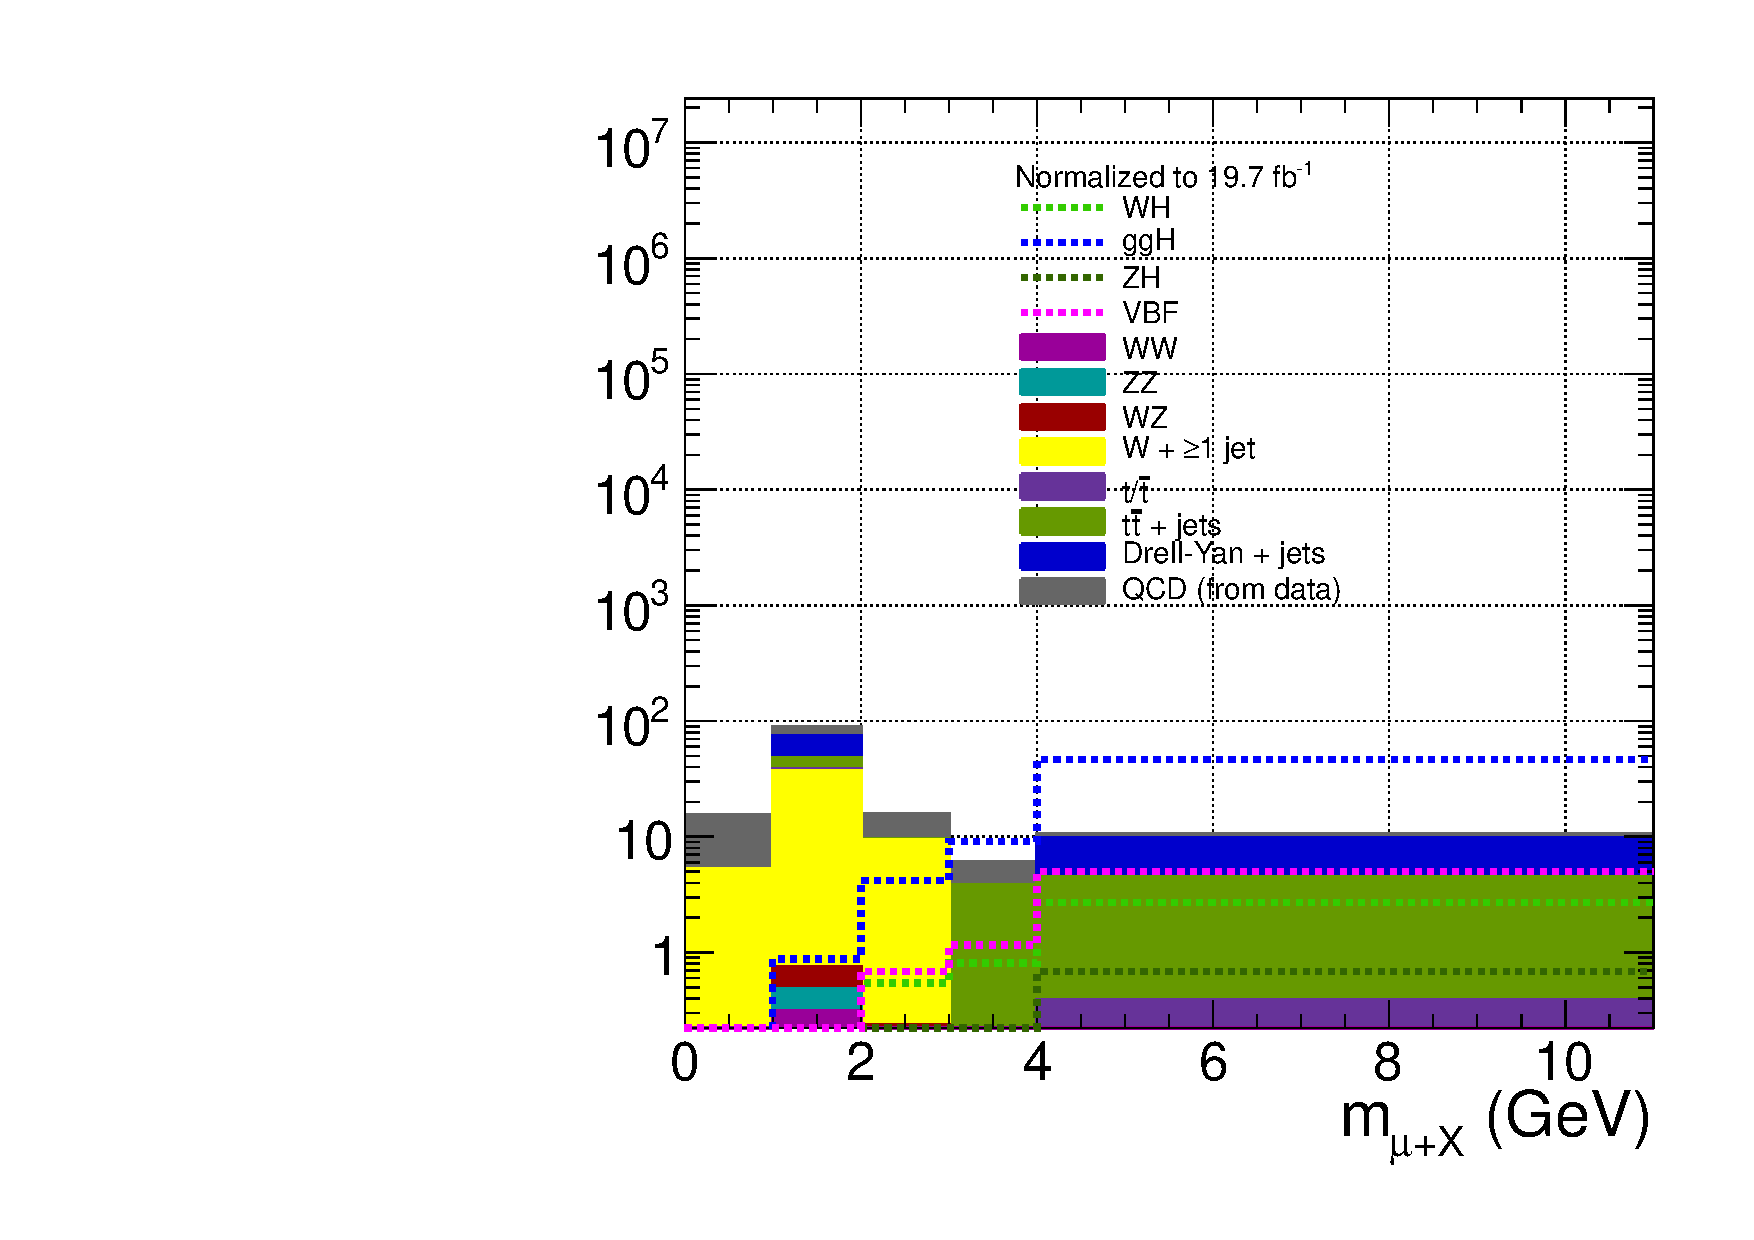
\includegraphics[width=\cmsFigWidth]{figures/sigVsBkg_muHadMass_lowMT_v87}
    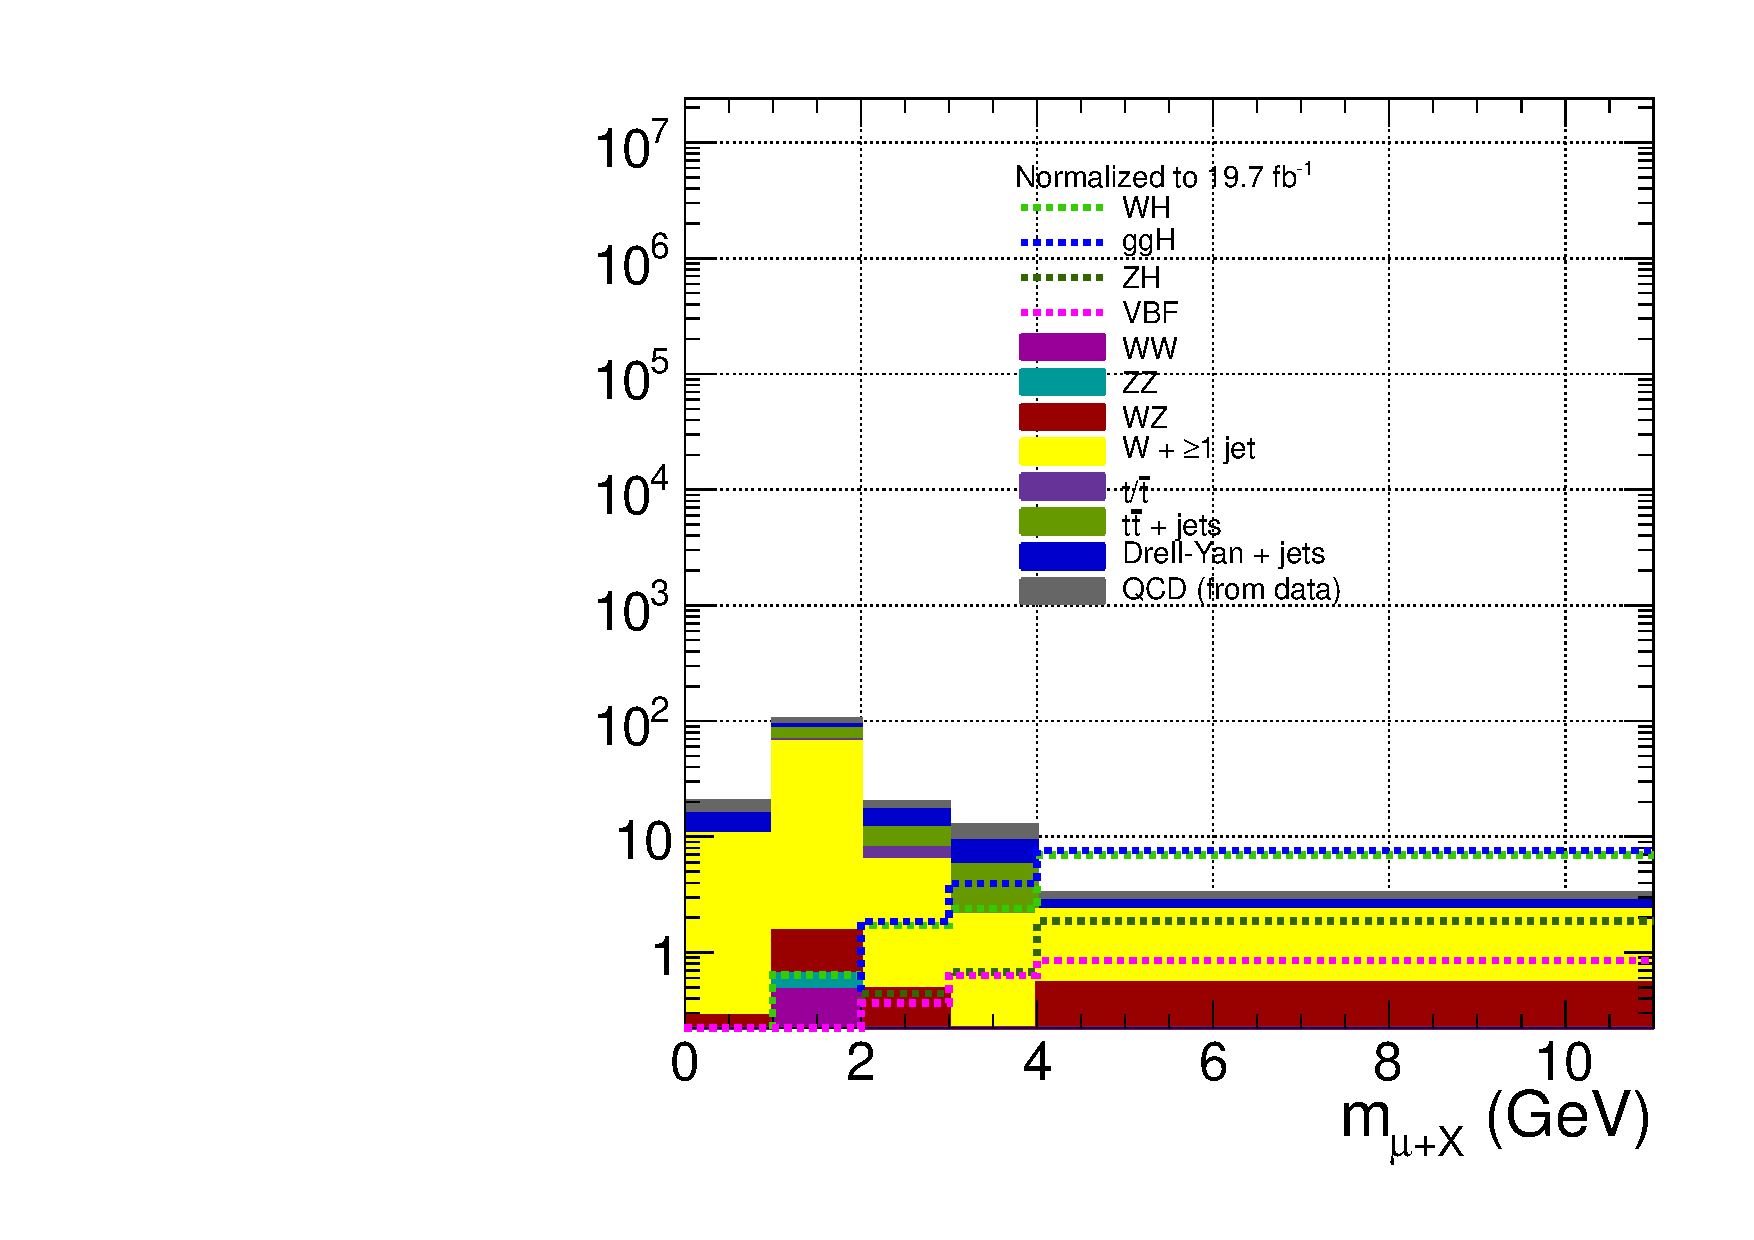
\includegraphics[width=\cmsFigWidth]{figures/sigVsBkg_muHadMass_highMT_v87}
    \caption{$m_{\mu+\text{had}}$ distribution after the preselection has been applied for four signal models and all backgrounds. Normalized to 19.7 fb$^{-1}$. (\cmsLeft) Low-$M_{T}$ bin. (\cmsRight) High-$M_{T}$ bin.}
    \label{fig:muhad-mass-MC-region-A}
  \end{center}
\end{figure}

This search is a blinded counting experiment in the signal region (``region A'', cf. Figure~\ref{fig:regionsAB}) defined by the cuts described in Chapter~\ref{sec:evtsel} plus $m_{\mu+\text{had}}$ $\geq$ 4 GeV.  The value of 4 GeV has been roughly optimized for the signal-to-background ratio by eyeballing the distributions of $m_{\mu+\text{had}}$.

\begin{figure}[hbtp]
  \begin{center}
    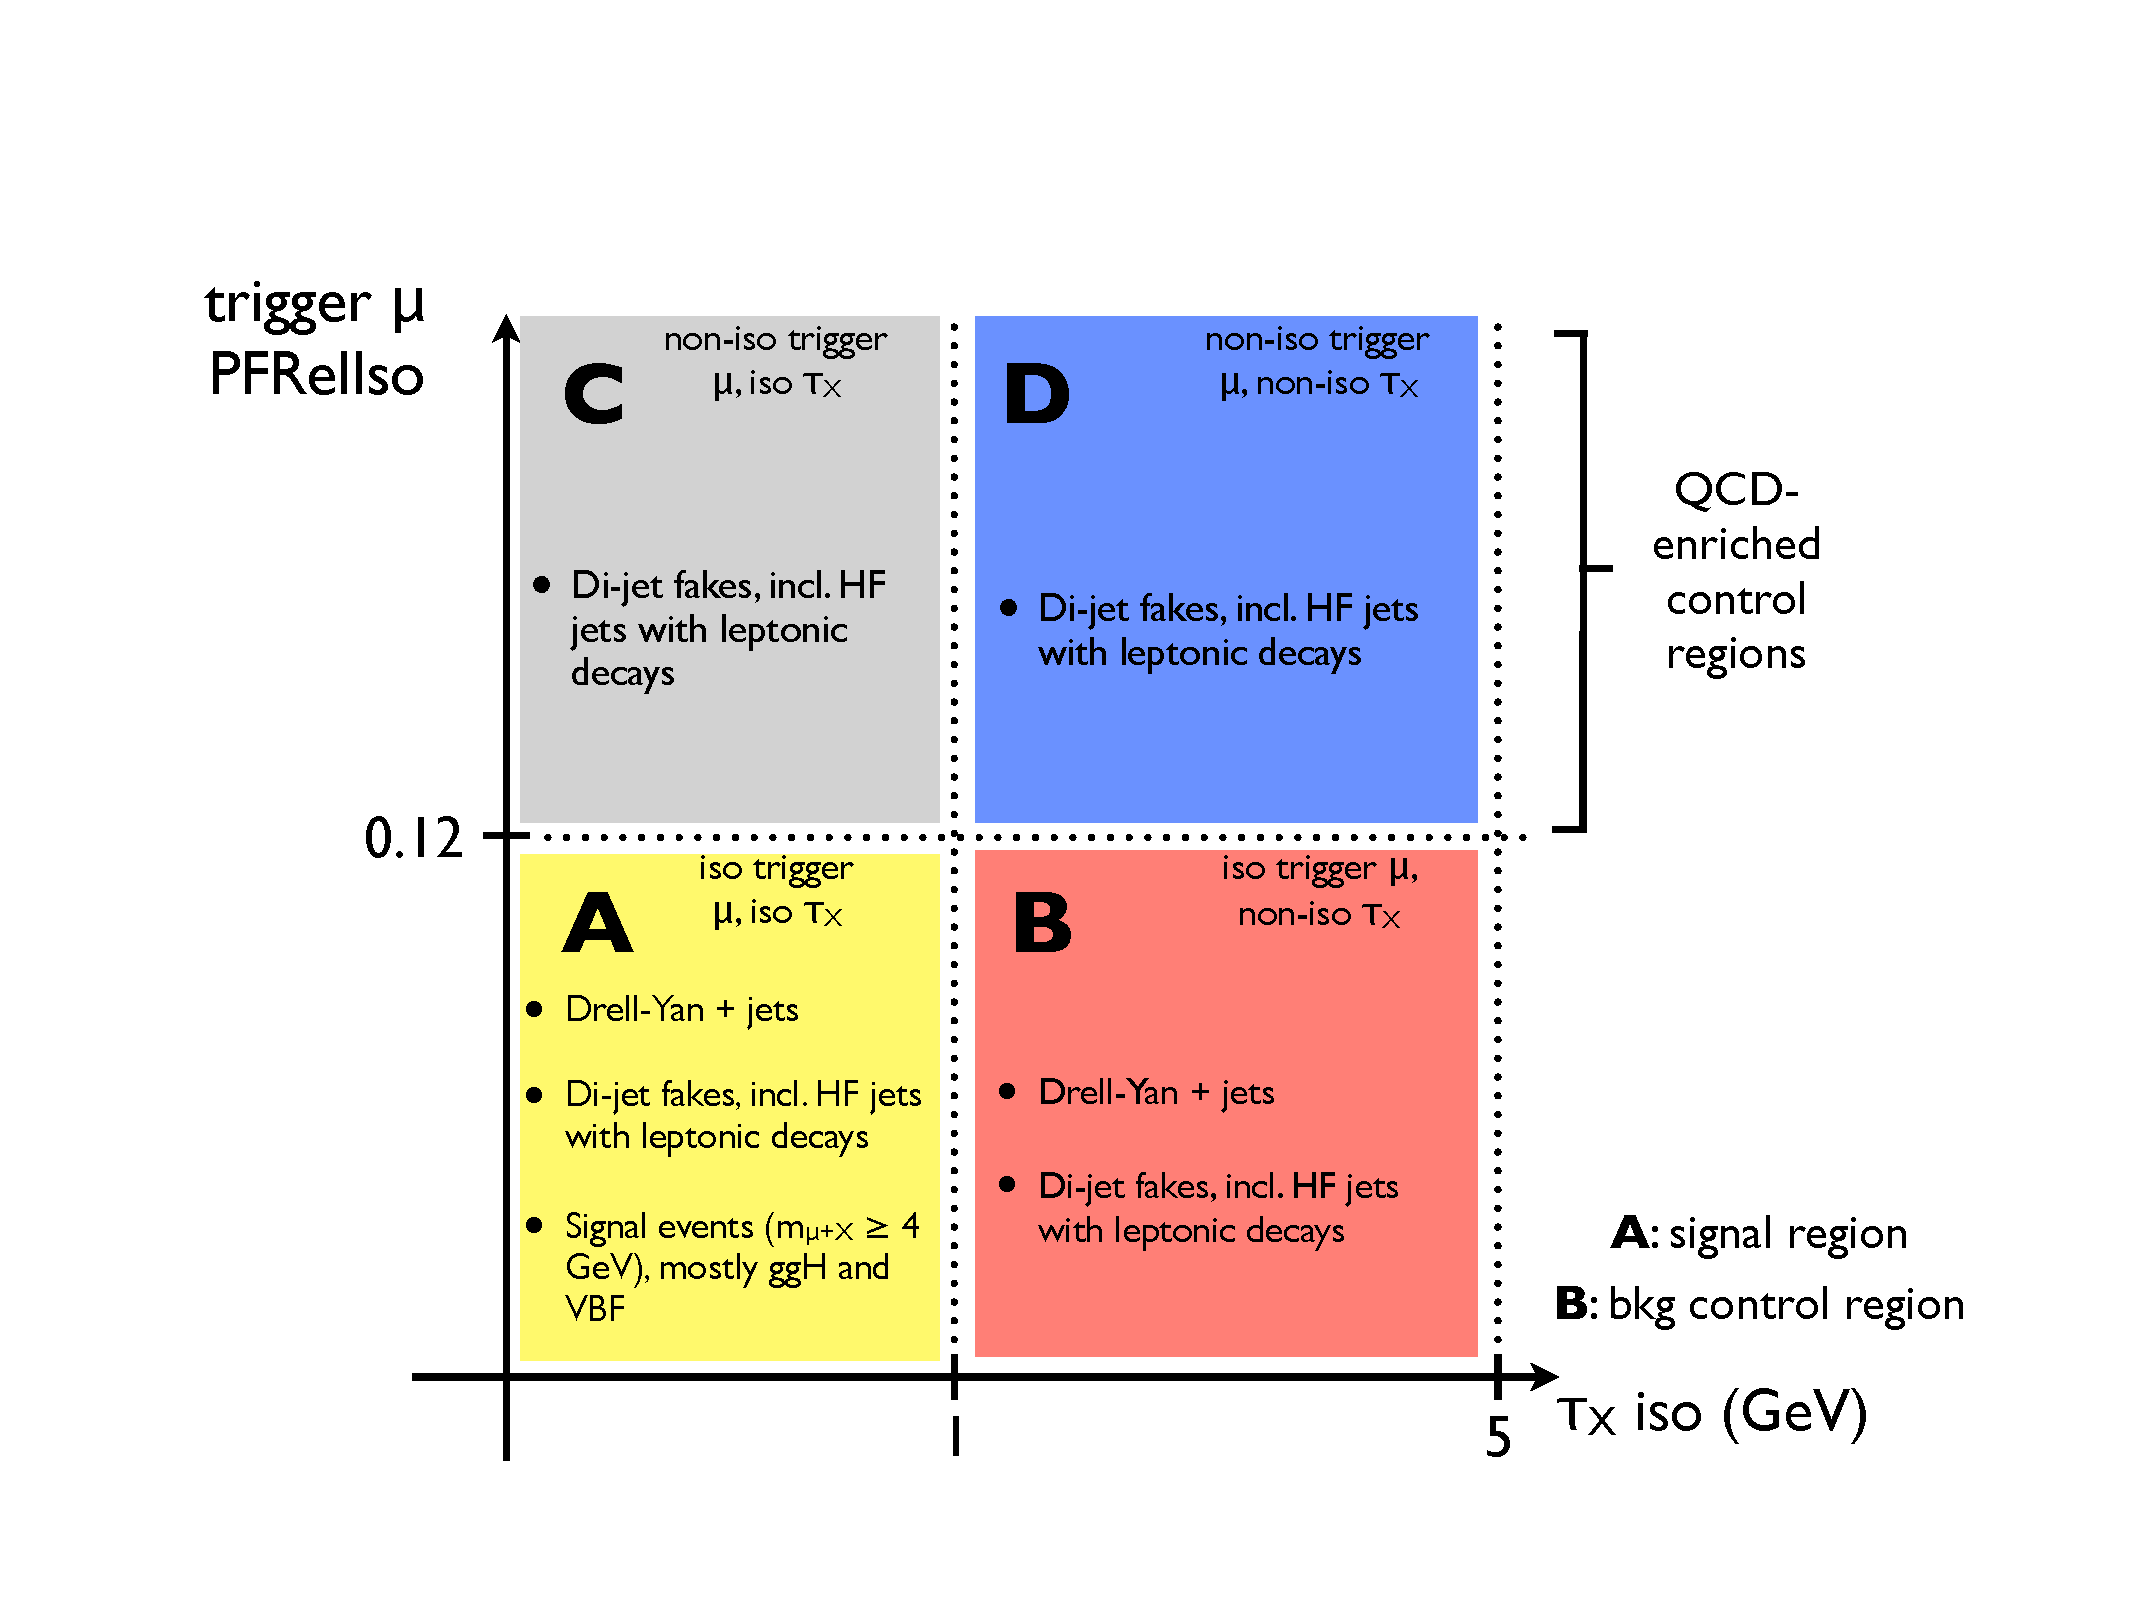
\includegraphics[width=2\cmsFigWidth]{figures/ABCD_annotated_lowMT}
    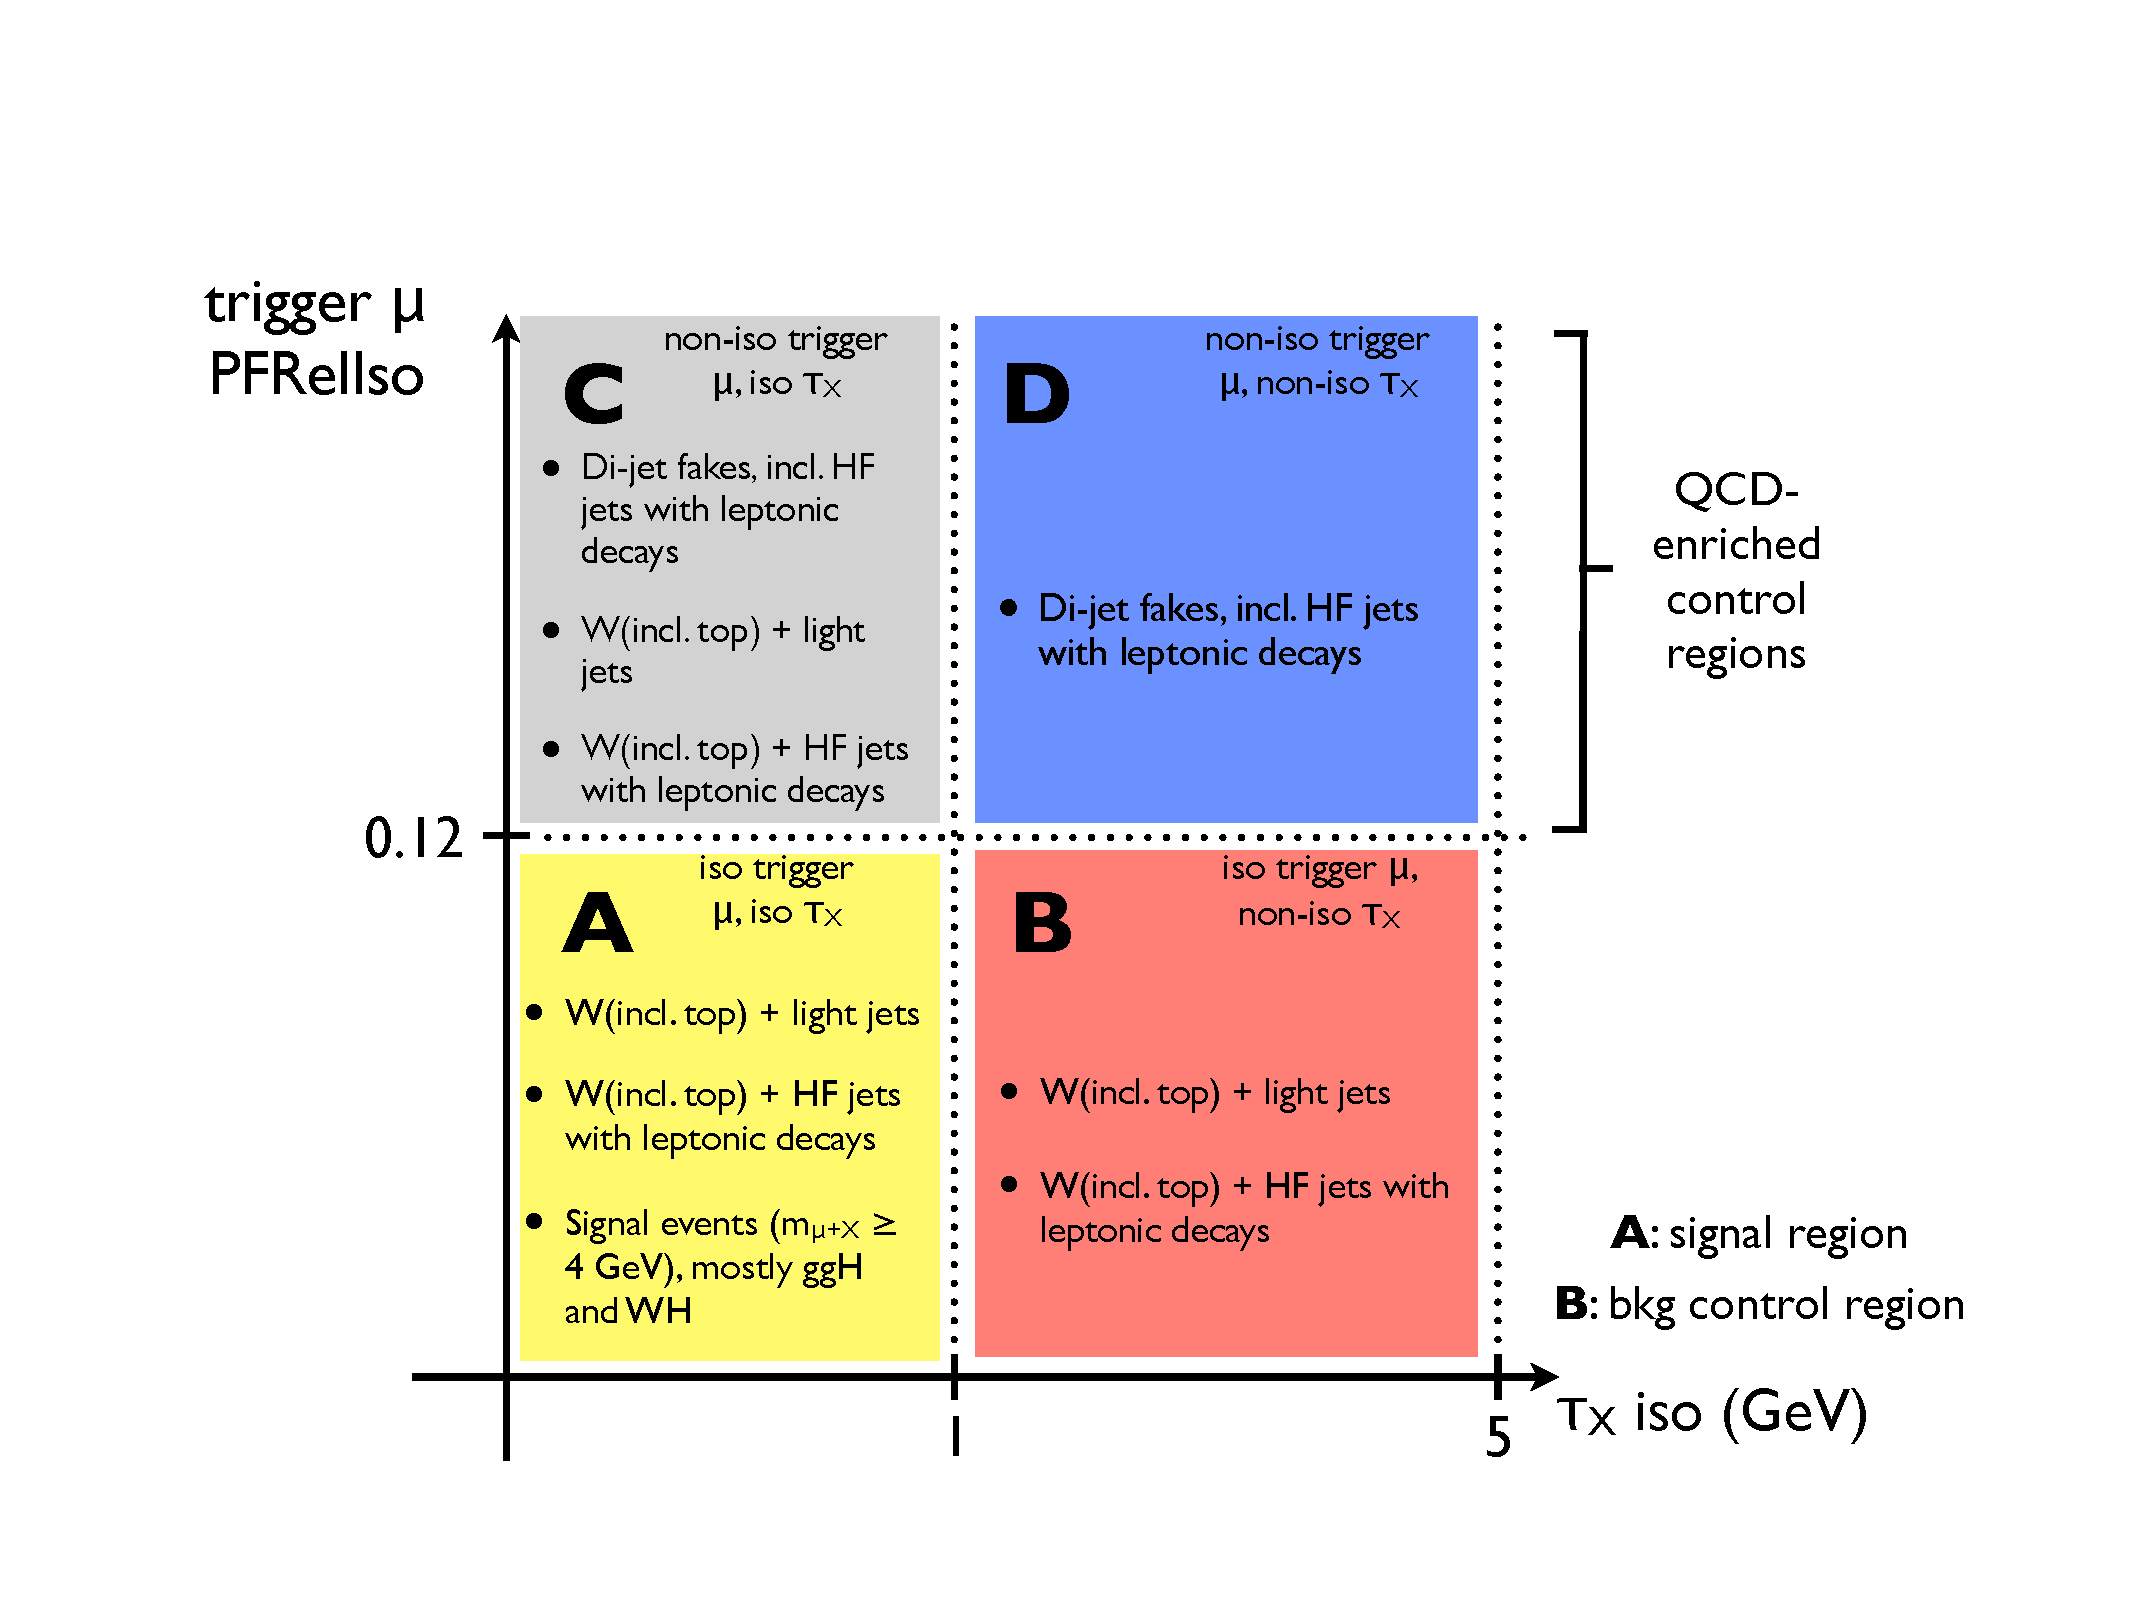
\includegraphics[width=2\cmsFigWidth]{figures/ABCD_annotated_highMT}
    \caption{Schematic description of the signal and control regions in this search. Signal region A is defined by HPS $\tau$ isolation between 0 and 1 GeV, after events have passed all other preselection cuts detailed in Chapter~\ref{sec:evtsel}. Likewise, jet fake control region B is defined by HPS $\tau$ isolation between 1 and 5 GeV, after events have passed all other preselection cuts. Regions C and D, which are enriched in QCD events, including those with double $\mu$ decays, are identical to regions A and B respectively, except that the trigger $\mu$ fails the tight isolation requirement and the neighbouring lepton filter is not imposed.  (Top) Low $M_{\text{T}}$.  (Bottom) High $M_{\text{T}}$.}
    \label{fig:regionsAB}
  \end{center}
\end{figure}

The background shape is derived from a single control sample defined from the $\tau_{\text{had}}$ isolation sideband (``region B", cf. Figure~\ref{fig:regionsAB}).  It describes the shape of the background due to light jets or jets with single muon decays mis-reconstructed as $\tau_{\mu}\tau_{\text{had}}$ pairs (``jet fakes"). The signal-depleted sideband $m_{\mu+\text{had}}$ $<$ 2 GeV is used to normalize the $m_{\mu+\text{had}}$ distribution from the jet fake control sample to data passing all the cuts described in Chapter~\ref{sec:evtsel}.  This gives the nominal background prediction $N_{\text{fake; pred}}^{\text{A}}$ for signal region A; the final background prediction in the search region $m_{\mu+\text{had}} >$ 4 GeV is obtained from the normalized region B distribution in the manner described later in Sec.~\ref{sec:bkgs-jet-fake-unc}, which factors in uncertainties in the background composition.
%The $m_{\mu+\text{had}}$ distribution from the jet fake control sample is normalized to data passing all the cuts described in Sec.~\ref{sec:evt-sel}, but in the signal-depleted subsample with $m_{\mu+\text{had}}$ $<$ 2 GeV.  This gives the total background prediction $N_{\text{fake; pred}}^{\text{A}}$ for signal region A.

The expected SM backgrounds differ in the low and high $M_{T}$ regions; in the high $M_{T}$ region, trigger muons mostly come from $W$'s, while in the low $M_{T}$ region, they mostly come from jets (including heavy flavor). However, in both regions, the backgrounds are dominated by events with a $\tau_{\mu}\tau_{\text{had}}$ object. Thus, the assumption is made that the shape of the background $m_{\mu+\text{had}}$ distributions in regions A and B are similar. To account for possible differences in the scaling factors of different contributions between regions A and B, studies were done to investigate the changes in shape based on varying these assumptions.

%jet fake bkg
\section{Jet fake background estimation\label{sec:bkg-jetfake}}

The data control sample used for estimating the jet fake background (``region B'') is defined by all of the cuts in Chapter~\ref{sec:evtsel}, except that the tau isolation is required to be between 1 and 5 GeV.  Table~\ref{tab:regA-vs-regB-def} gives the cut values defining the search region (tau isolation $\le$ 1 GeV); the cuts defining the jet fake control region are all identical except for the cut on tau isolation.

\begin{table*}[htbH]
\begin{center}
\caption{Cut values defining the data search region A. The cuts defining the jet fake control region B are all identical, except that for having tau isolation $>$1 GeV \&\& $<$5 GeV.\label{tab:regA-vs-regB-def}}
\singlespacing
\begin{tabular}{ll}
\hline Variable & Search region \\% & Control region \\
\hline
HLT & \begin{tabular}[c]{@{}l@{}}\texttt{HLT\_IsoMu24\_eta2p1}\\\texttt{\_v[1-15]}\end{tabular} \\% & \begin{tabular}[c]{@{}l@{}}\texttt{HLT\_IsoMu24\_eta2p1}\\\texttt{\_v[1-15]}\end{tabular} \\
First muon $p_T$ & $>$25 GeV \\% & $>$25 GeV \\
First muon $|\eta|$ & $<$2.1 \\% & $<$2.1 \\
First muon ID (cf. Sec.~\ref{sec:evtsel-triggermu}) & Tight \\% & Tight \\
First muon rel. iso. (cf. Sec.~\ref{sec:evtsel-triggermu}) & $<$0.12 \\% & $<$0.12 \\
\DR(First muon, PF electron) (cf. Sec.~\ref{sec:evtsel-leptonveto}) & $>$0.4 \\% & $>$0.4 \\
\DR(First muon, soft muon) (cf. Sec.~\ref{sec:evtsel-leptonveto}) & $>$0.4 \\%& $>$0.4 \\
\DR(First muon, PF tau) (cf. Sec.~\ref{sec:evtsel-leptonveto}) & $>$0.4 \\%& $>$0.4 \\
\DR(first muon, HLT object) & $<$0.1 \\%& $<$0.1 \\
Second muon $p_T$ & $>$5 GeV \\%& $>$5 GeV \\
Second muon $\abs{\eta}$ & $<$2.1 \\%& $<$2.1 \\
Second muon ID (cf. Sec.~\ref{sec:evtsel-softmu}) & Soft \\%& Soft \\
Second muon $\neq$ first muon & True \\%& True \\
$q$(second muon) $\times$ $q$(first muon) & $>$0 \\%& $>$0 \\
\begin{tabular}[c]{@{}l@{}}Tau reco'd from jet cleaned \\of second muon (cf. Sec.~\ref{sec:evtsel-tauID})\end{tabular} & True \\%& True \\
Tau $p_T$ & $>$20 GeV \\%& $>$20 GeV \\
Tau $|\eta|$ & $<$2.3 \\%& $<$2.3 \\
Tau decay mode finding (cf. Sec.~\ref{sec:evtsel-tauID}) & True \\%& True \\
Tau isolation (cf. Sec.~\ref{sec:evtsel-tauID}) & Medium ($\le$1 GeV) \\%& $>$1 GeV \&\& $<$5 GeV \\
$q$(second muon) $\times$ $q$(tau) & =0 \\%& =0 \\
$\cPqb$ jet veto (cf. Sec.~\ref{sec:evtsel-bveto}) & CSVM \\%& CSVM \\
$d_{\text{z}}$($\tau_{\mu}$,PV) (cf. Sec.~\ref{sec:evtsel-dz}) & $<$0.5 cm \\%& $<$0.5 cm \\
$d_{\text{z}}$($\tau_{\text{had}}$,PV) (cf. Sec.~\ref{sec:evtsel-dz}) & $<$0.2 cm \\%& $<$0.2 cm \\
\hline
\end{tabular}
\end{center}
\end{table*}

%Subsection: Region B vs A shape validation
\subsection{Validation of similarity of background shapes in isolated and non-isolated tau regions\label{sec:bkgs-test-MC}}

For the Drell-Yan, $W$ + jets, top, and di-boson backgrounds, MC is used to check how well the jet fake control sample (region B) defined in Table~\ref{tab:regA-vs-regB-def} is expected to predict the shape of the $m_{\mu+\text{had}}$ distribution due to jet fakes in the search sample (region A).  For each of the MC samples described in Table~\ref{tab:MCBkg}, comparisons of the shapes of the $m_{\mu+\text{had}}$ distributions between samples of events passing the search region (A) cuts and those passing the control region (B) cuts are shown in Figures~\ref{fig:MC-regA-vs-regB-main-lowMT} and~\ref{fig:MC-regA-vs-regB-secondary-lowMT} for the low-$M_{\text{T}}$ bin and in Figures~\ref{fig:MC-regA-vs-regB-main-highMT} and~\ref{fig:MC-regA-vs-regB-secondary-highMT} for the high-$M_{\text{T}}$ bin. These figures show only the shape comparisons for the individual background sources without any information about their relative ratios in regions A and B; to validate the similarity of the overall background shapes in regions A and B, a comparison of the sum of the MC backgrounds is shown in Figures~\ref{fig:MC-regA-vs-regB-lowMT} and~\ref{fig:MC-regA-vs-regB-highMT}.

\begin{figure}[hbtp]
  \begin{center}
    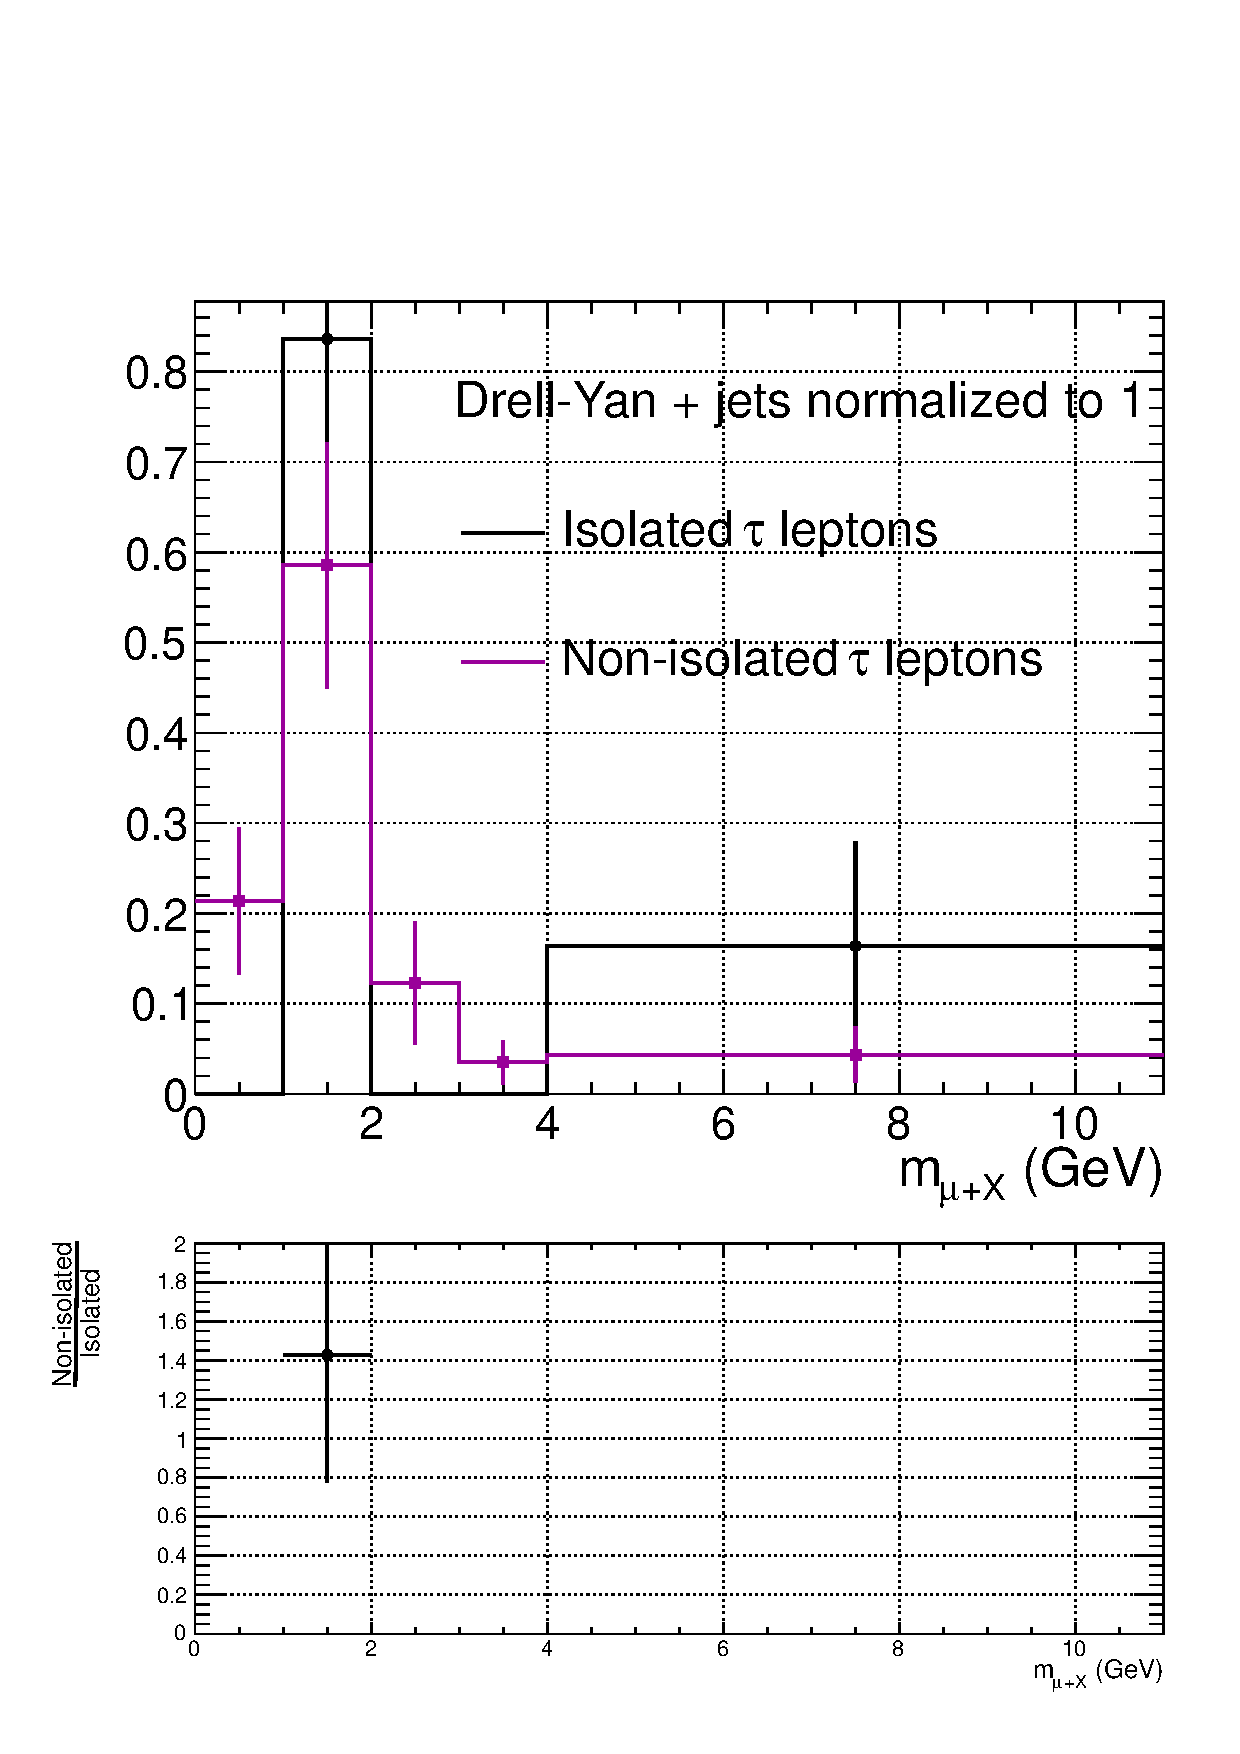
\includegraphics[width=0.8\cmsFigWidth]{figures/isoVsNonIsoTaus_DY_lowMT_v87}
    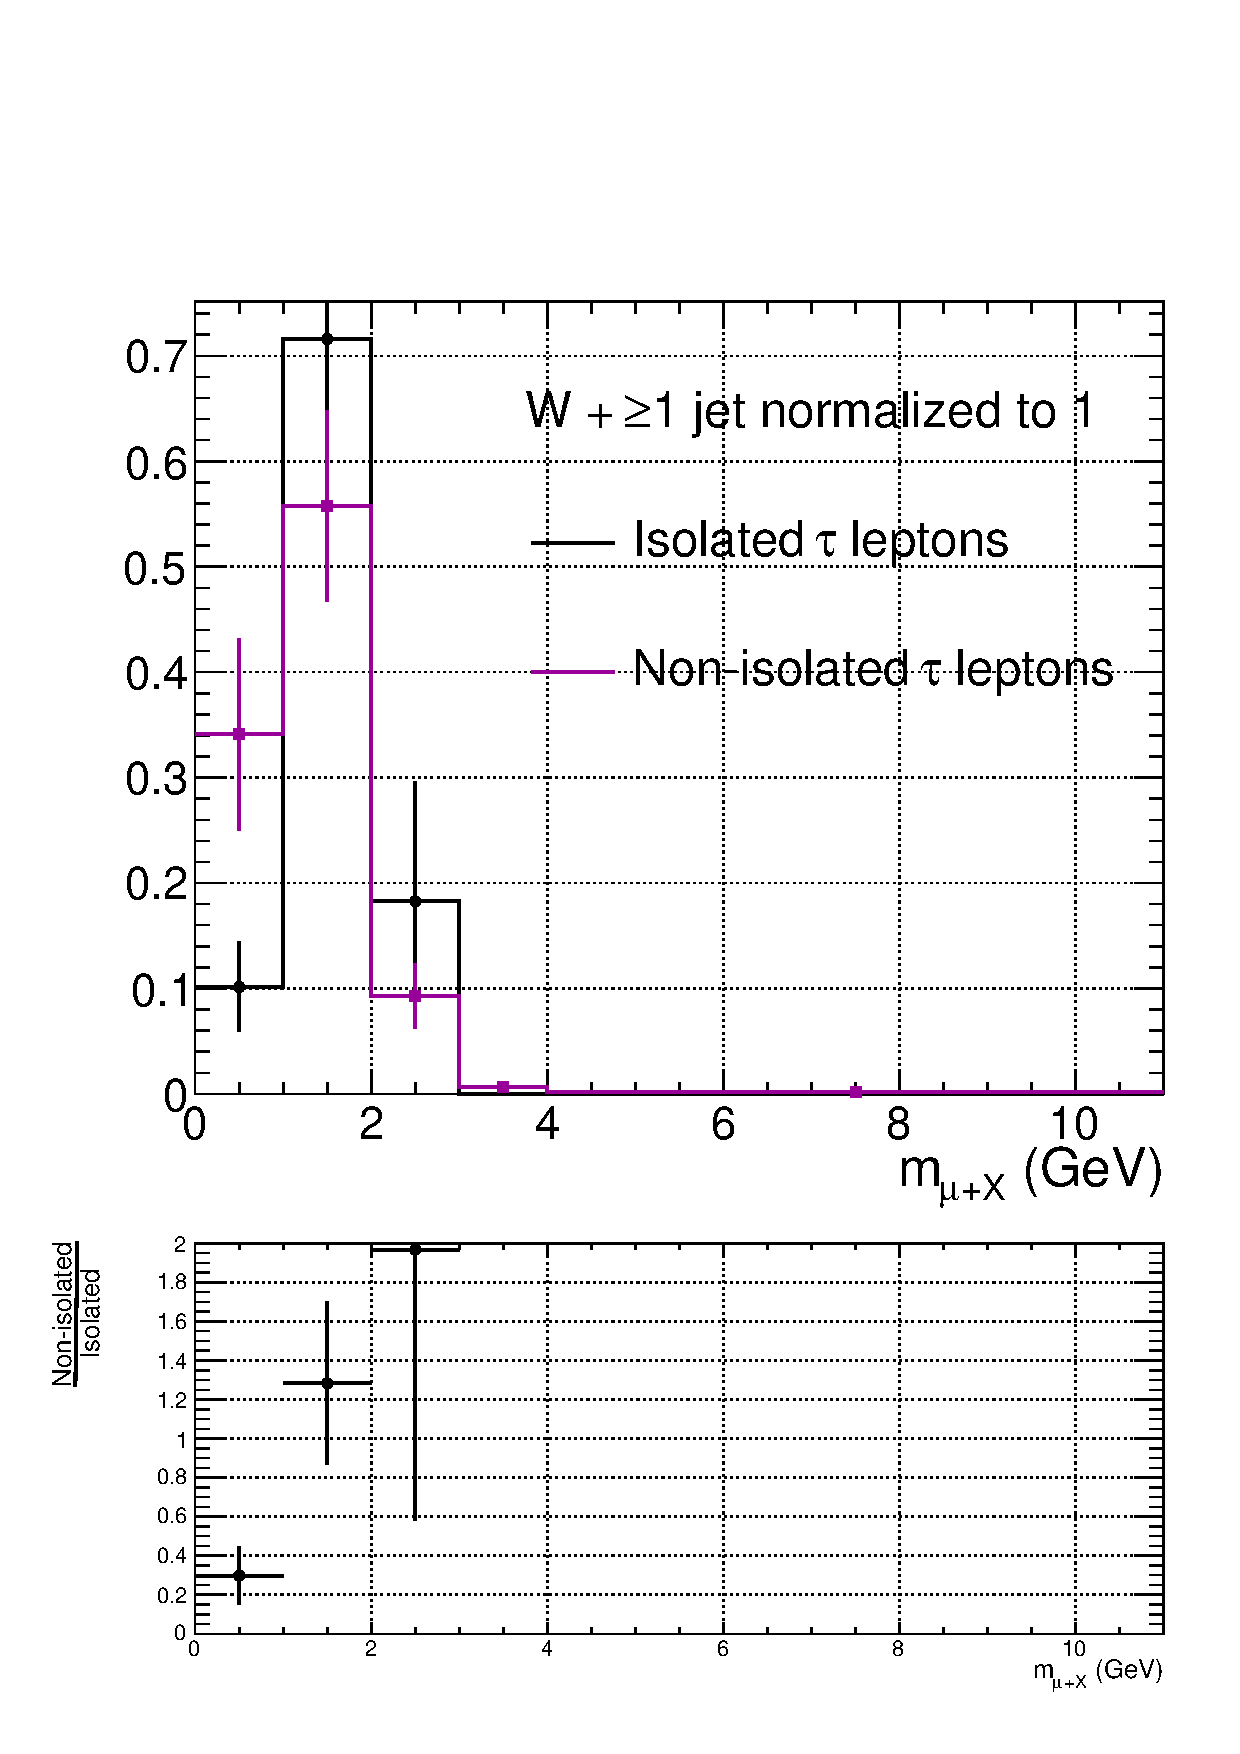
\includegraphics[width=0.8\cmsFigWidth]{figures/isoVsNonIsoTaus_WNJets_lowMT_v87}
    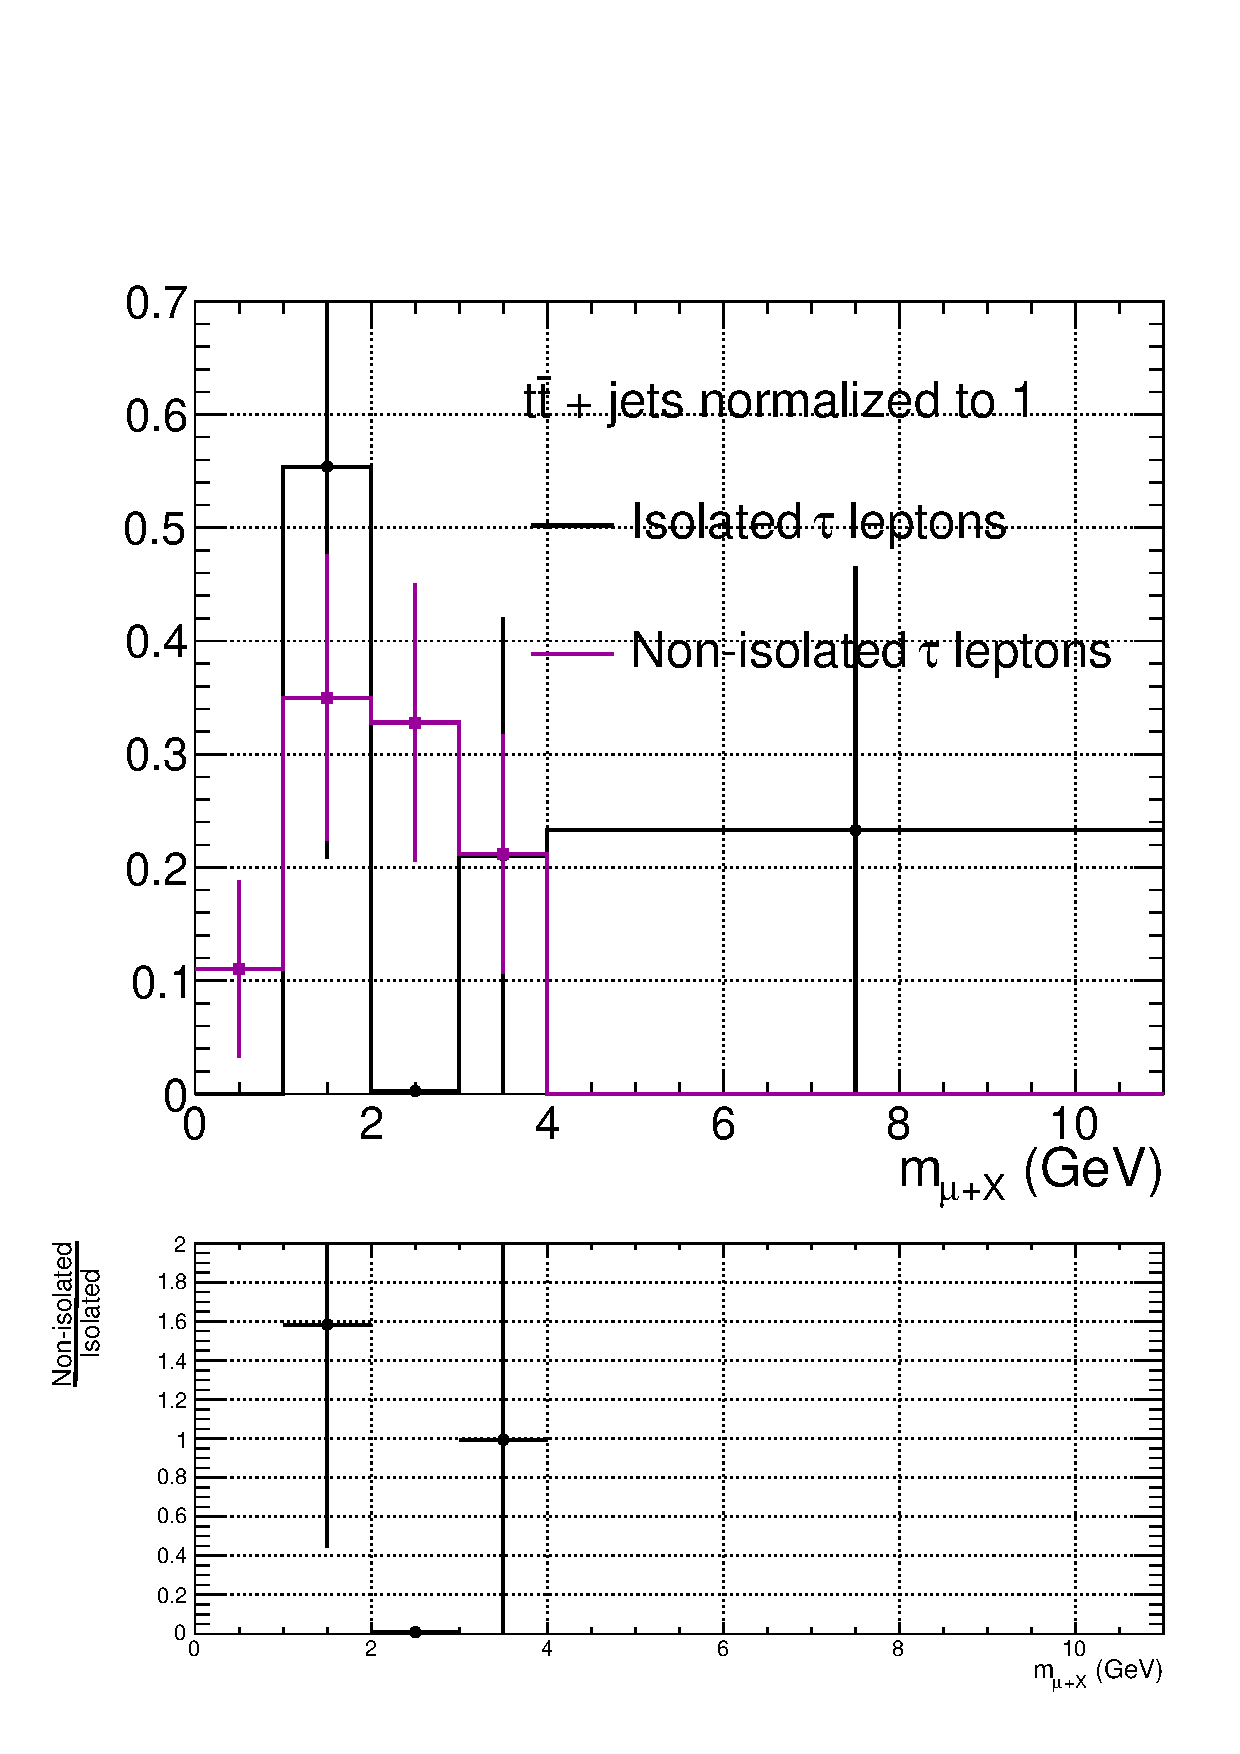
\includegraphics[width=0.8\cmsFigWidth]{figures/isoVsNonIsoTaus_TTJets_lowMT_v87}
    \caption{$m_{\mu+\text{had}}$ distributions in the low-$M_{\text{T}}$ bin, normalized to one, for MC events passing the search region selection (black) and the jet fake control region selection (purple).  The small plots beneath the main plots show the ratio of the control region distribution to the search region distribution.  Errors are statistical only.  (\cmsLeft) Drell-Yan.  (Middle) $W$ + $\ge$1 jet.  (\cmsRight) $t\bar{t}$.}
    \label{fig:MC-regA-vs-regB-main-lowMT}
  \end{center}
\end{figure}

\begin{figure}[hbtp]
  \begin{center}
    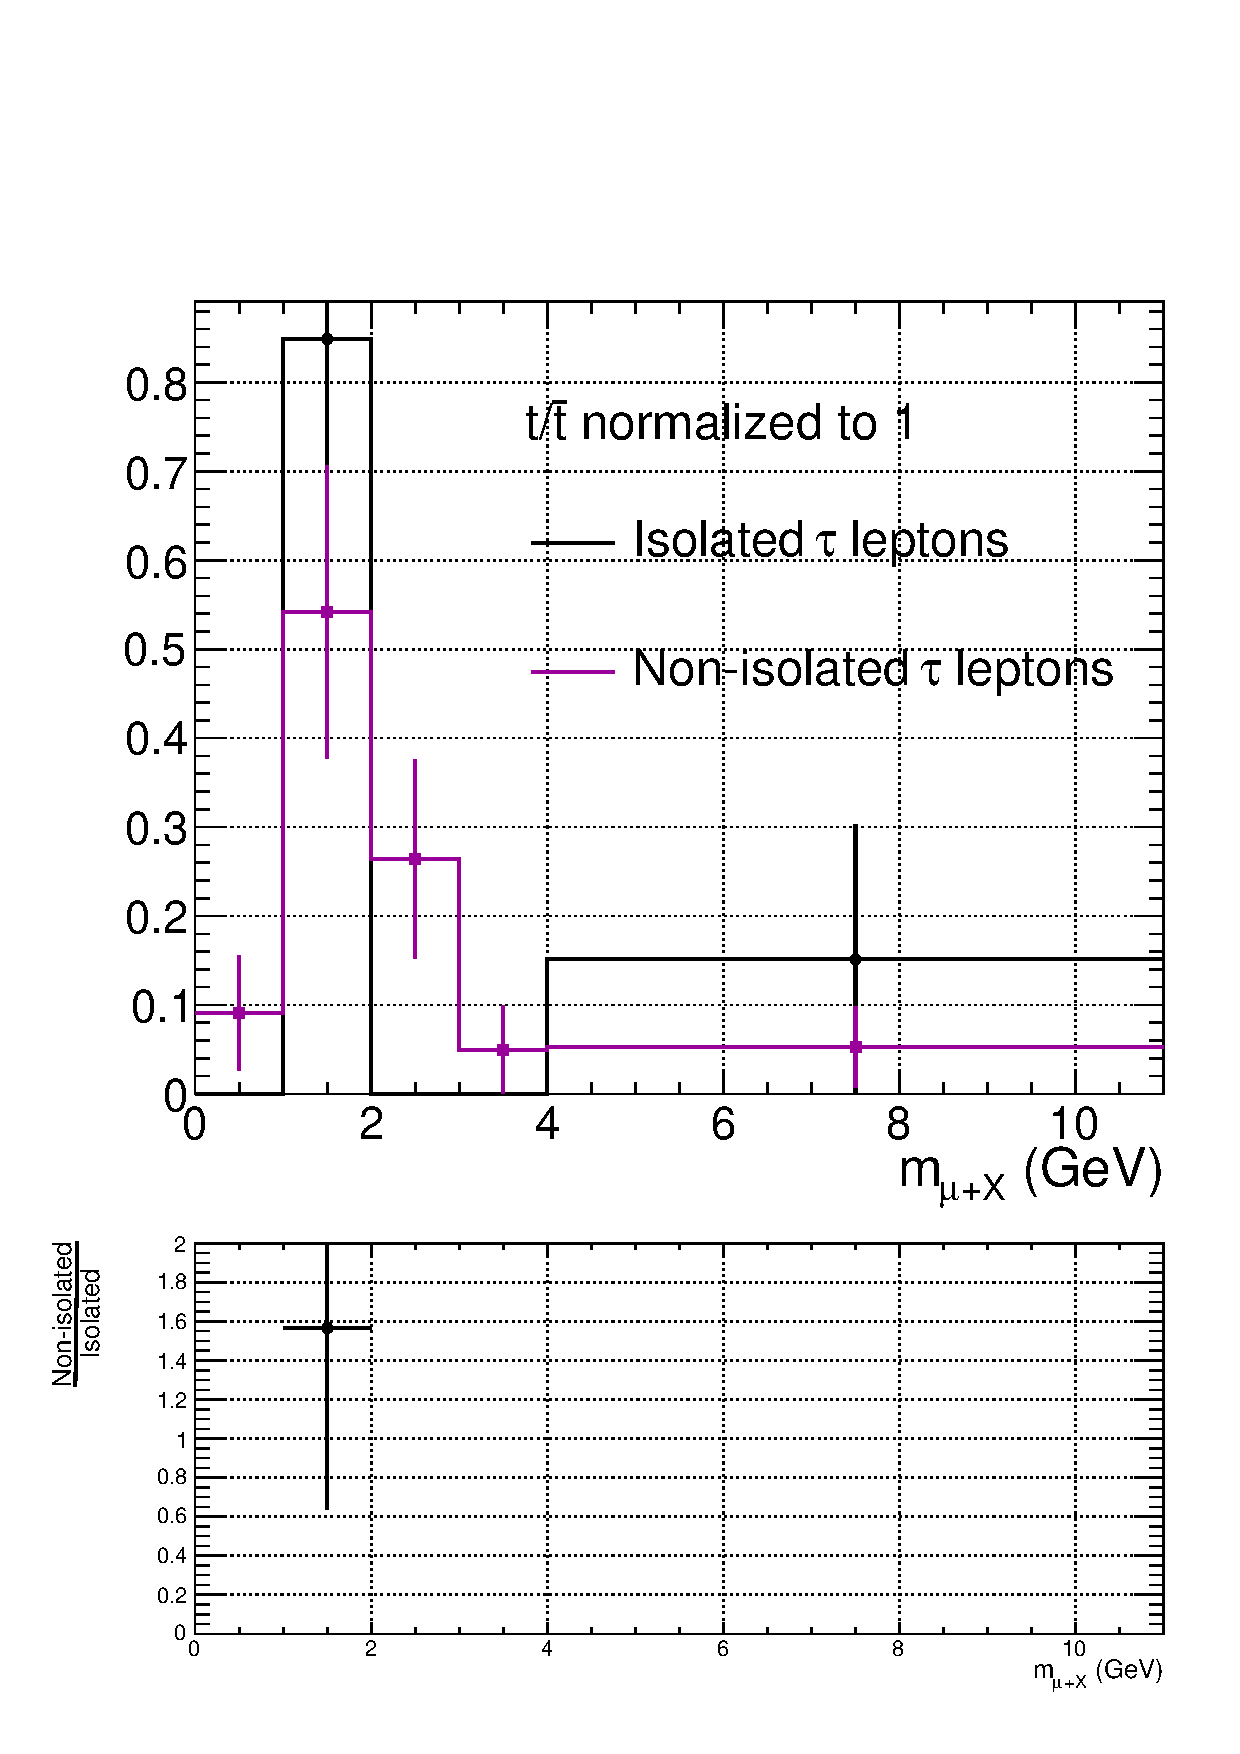
\includegraphics[width=0.6\cmsFigWidth]{figures/isoVsNonIsoTaus_SingleTop_lowMT_v87}
    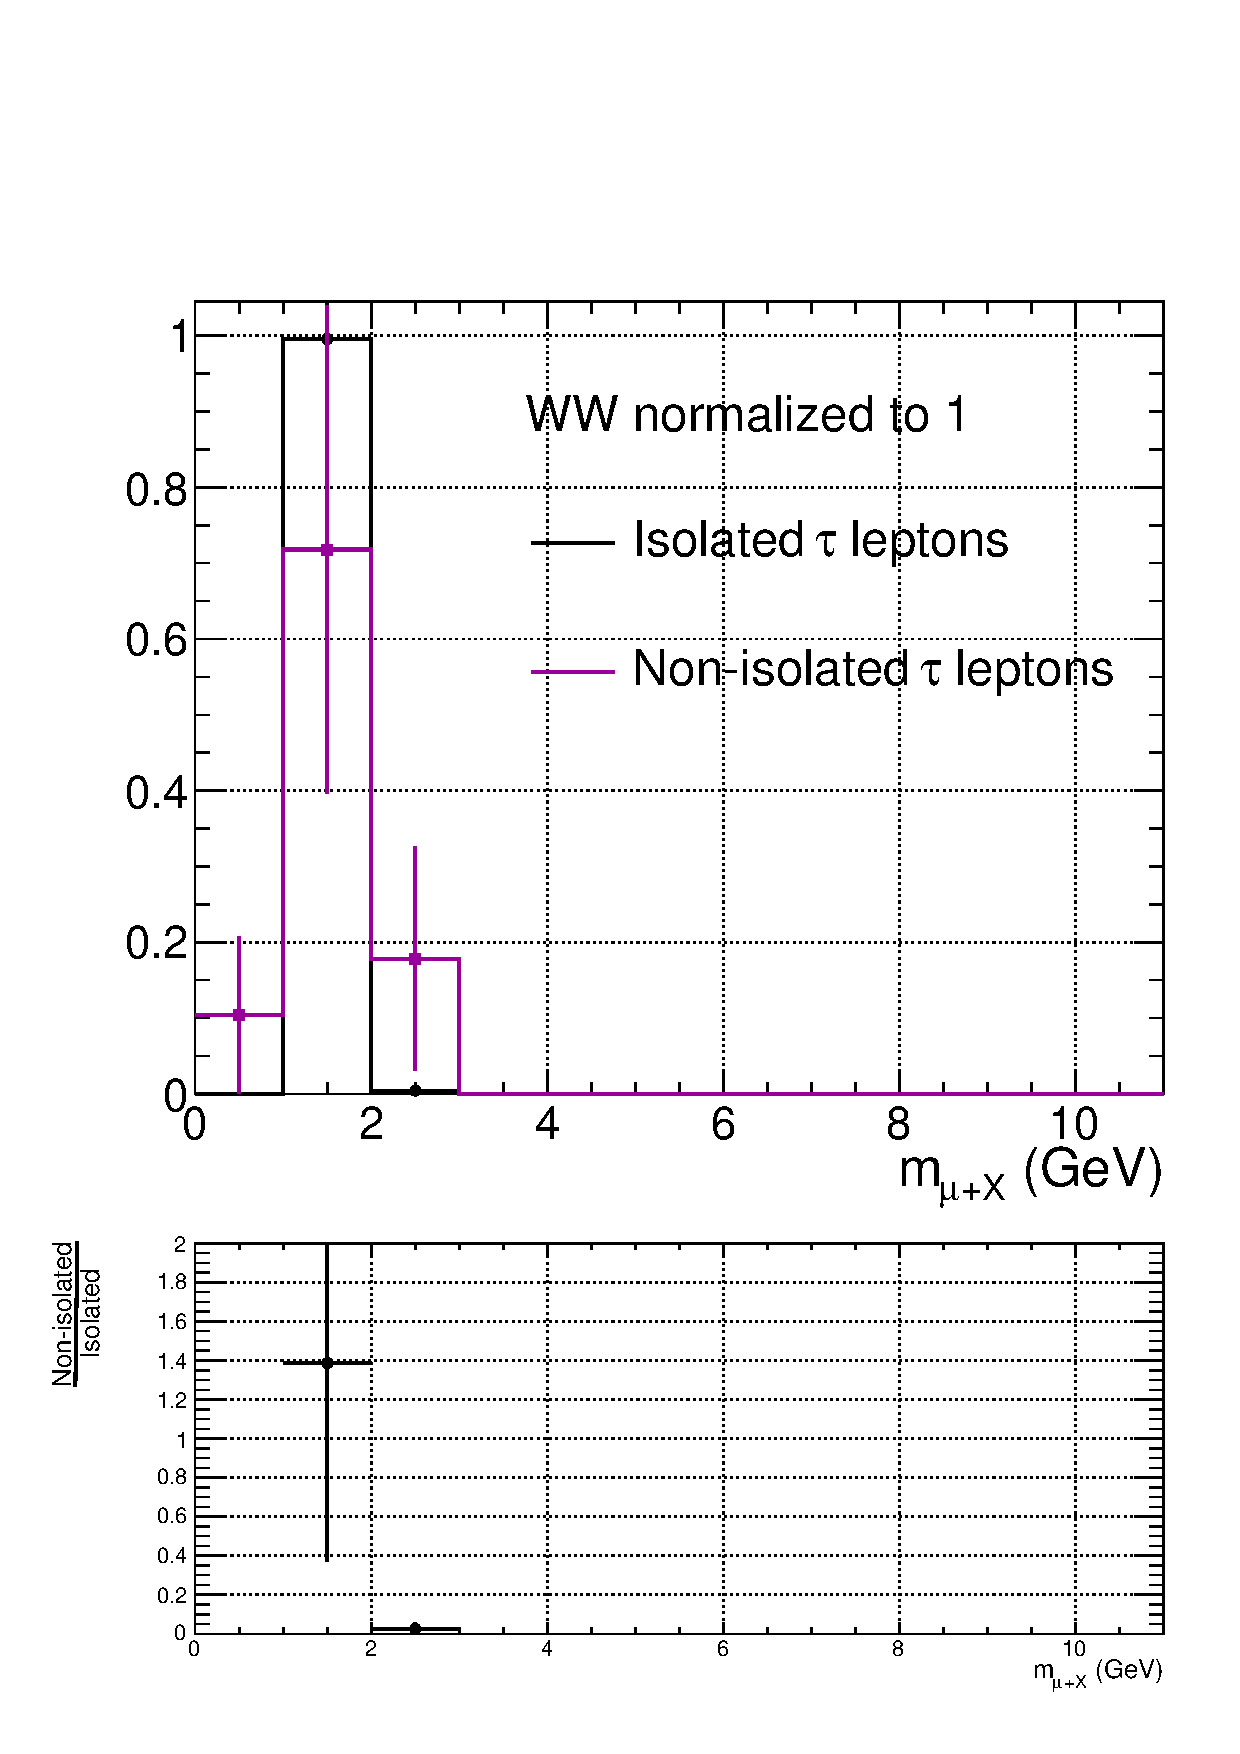
\includegraphics[width=0.6\cmsFigWidth]{figures/isoVsNonIsoTaus_WW_lowMT_v87}
    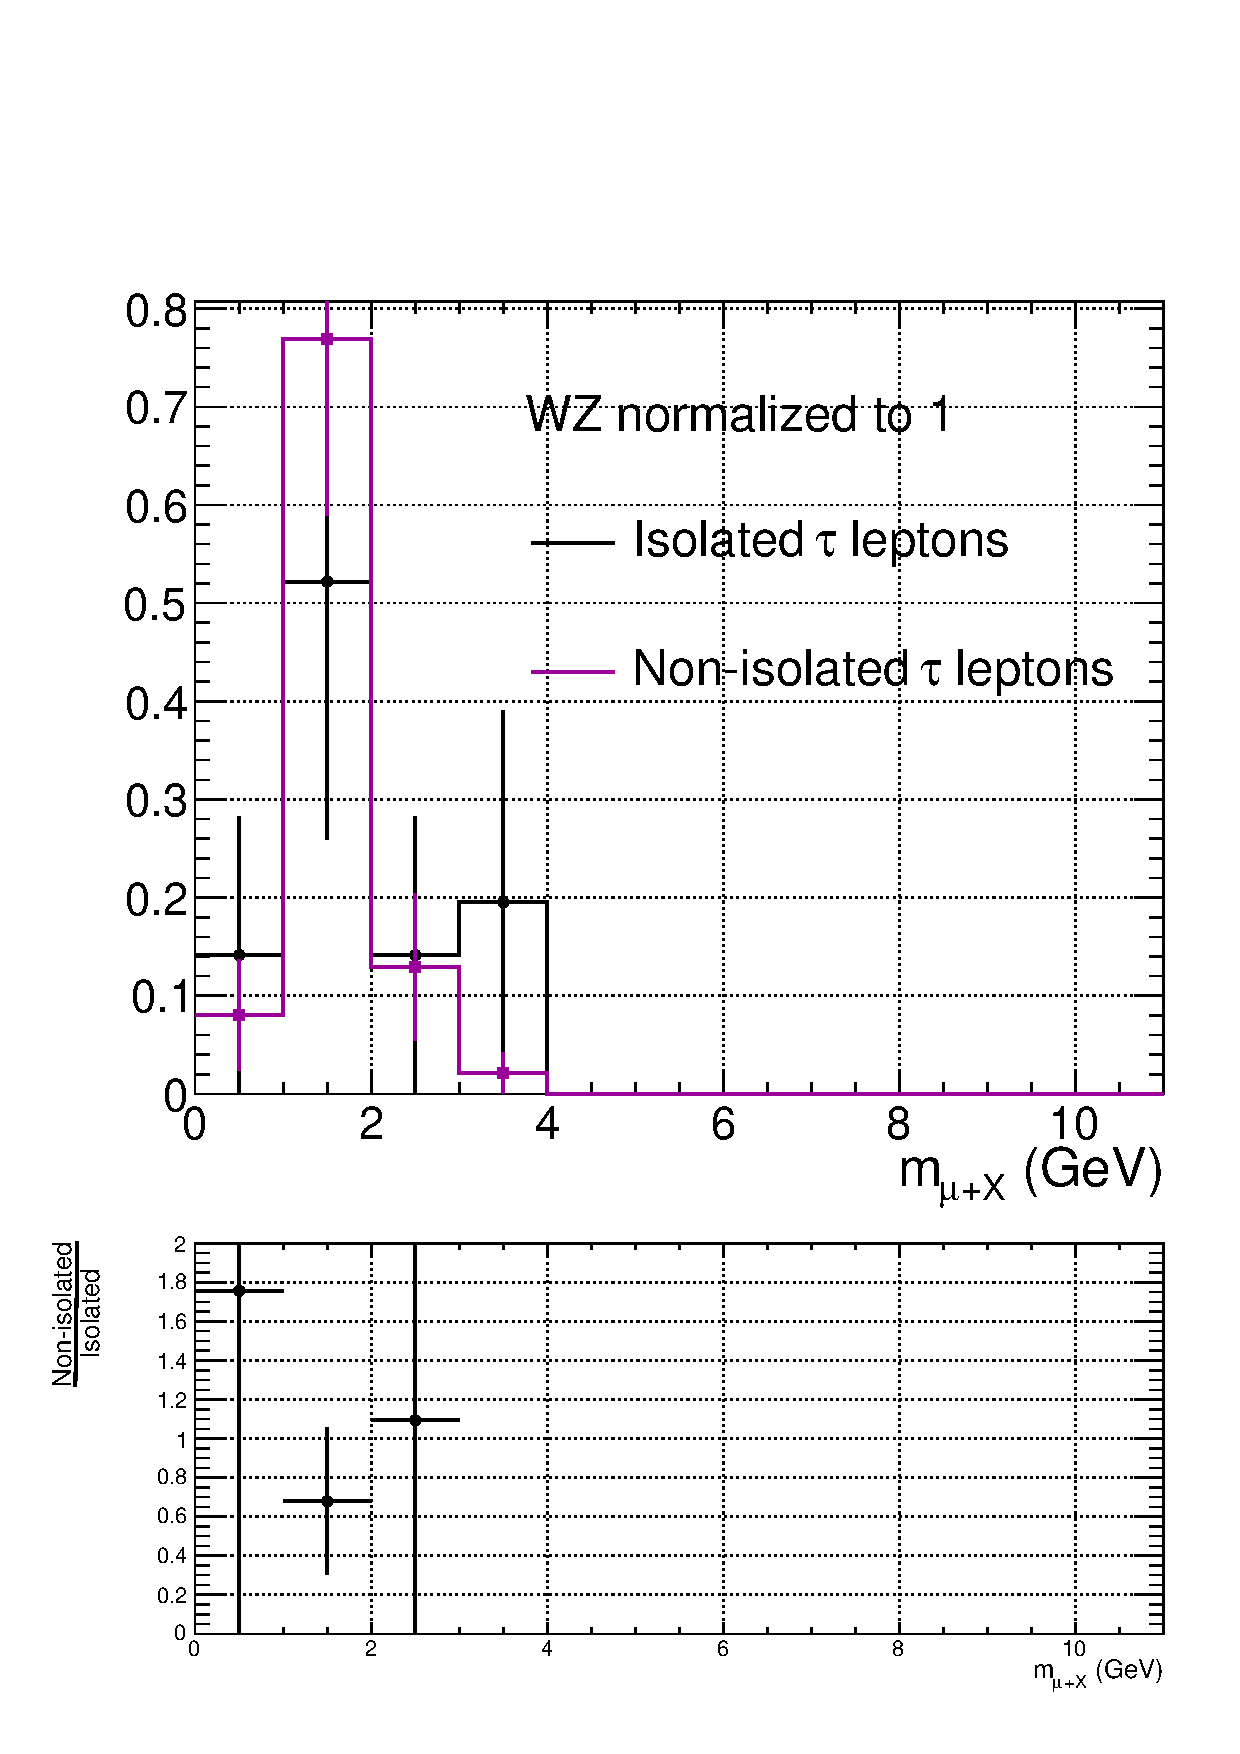
\includegraphics[width=0.6\cmsFigWidth]{figures/isoVsNonIsoTaus_WZ_lowMT_v87}
    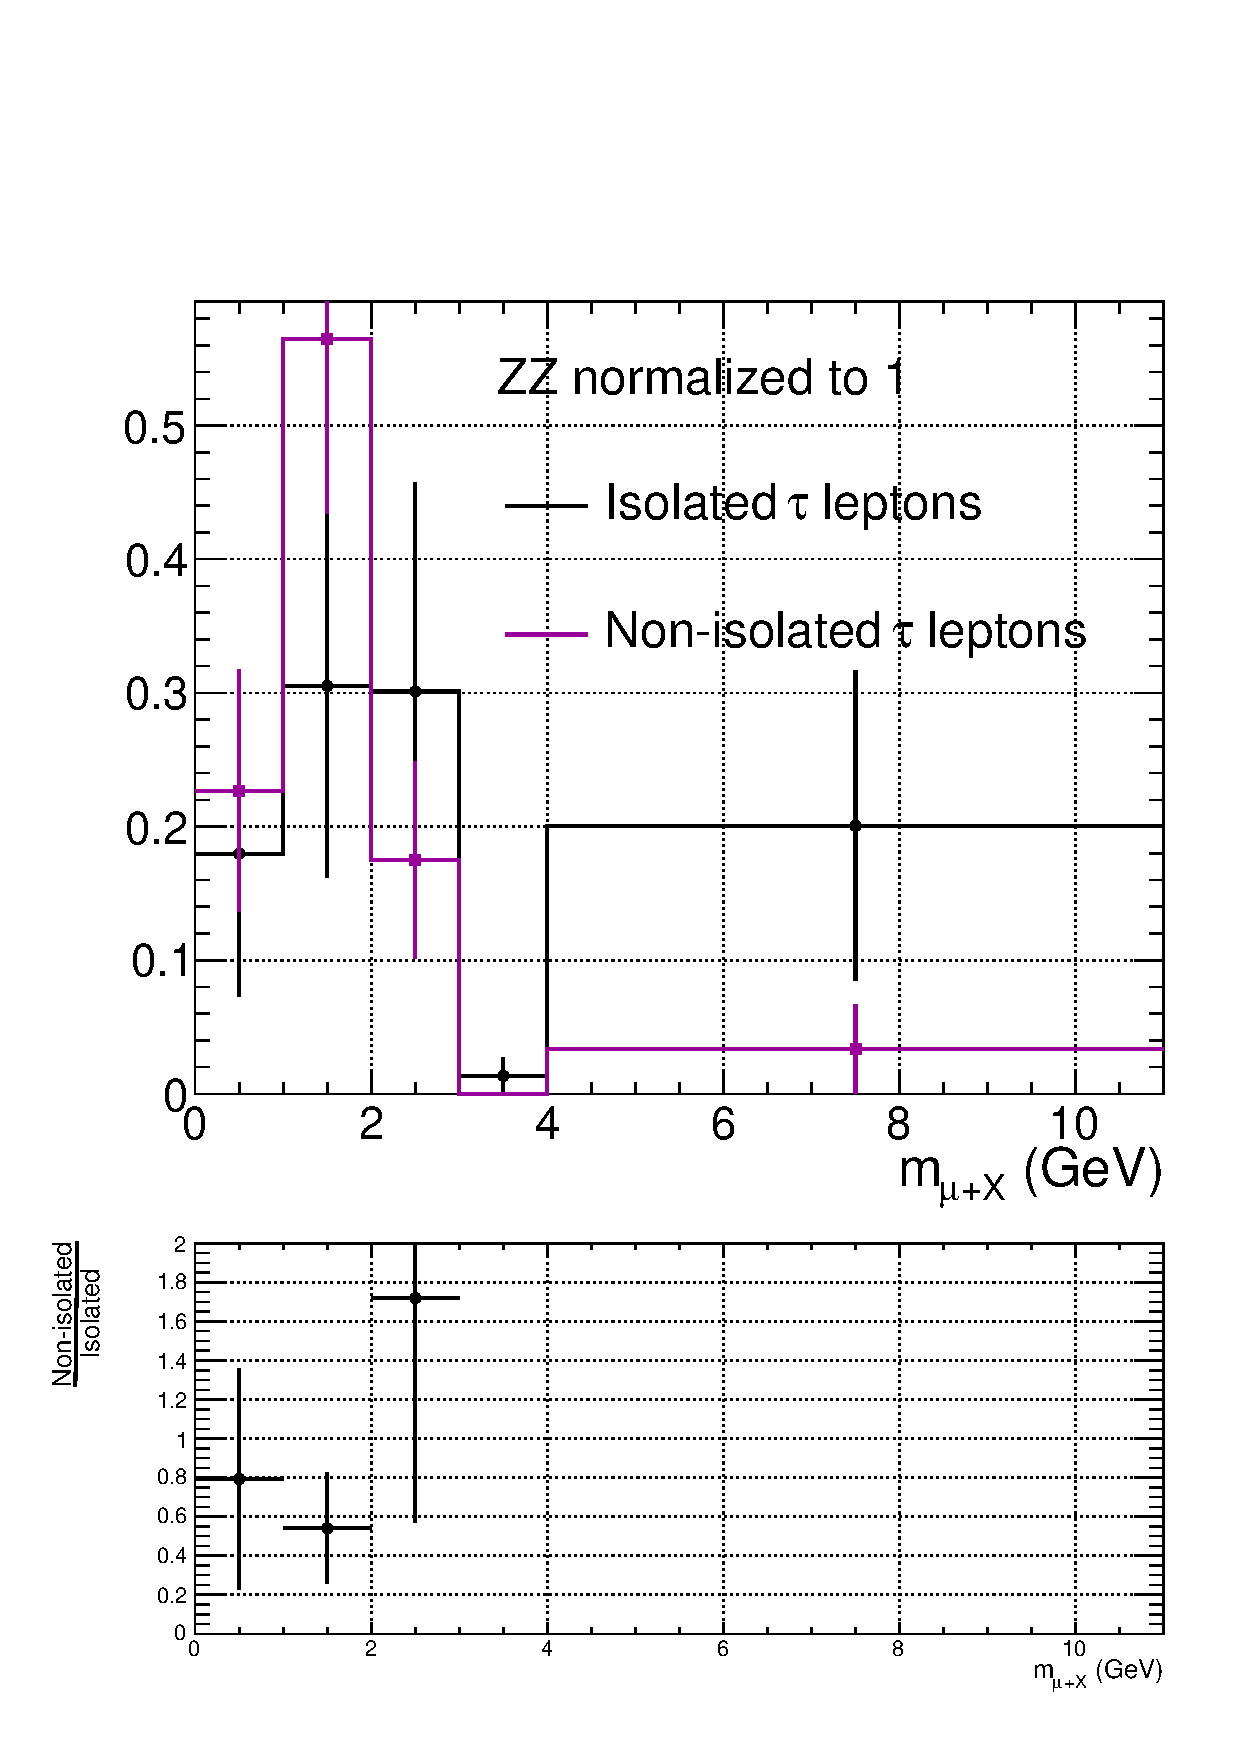
\includegraphics[width=0.6\cmsFigWidth]{figures/isoVsNonIsoTaus_ZZ_lowMT_v87}
    \caption{$m_{\mu+\text{had}}$ distributions in the low-$M_{\text{T}}$ bin, normalized to one, for MC events passing the search region selection (black) and the jet fake control region selection (purple).  The small plots beneath the main plots show the ratio of the control region distribution to the search region distribution.  Errors are statistical only.  (\cmsLeft) Single top.  (Middle \cmsLeft) WW.  (Middle \cmsRight) WZ.  (\cmsRight) ZZ.}
    \label{fig:MC-regA-vs-regB-secondary-lowMT}
  \end{center}
\end{figure}

\begin{figure}[hbtp]
  \begin{center}
    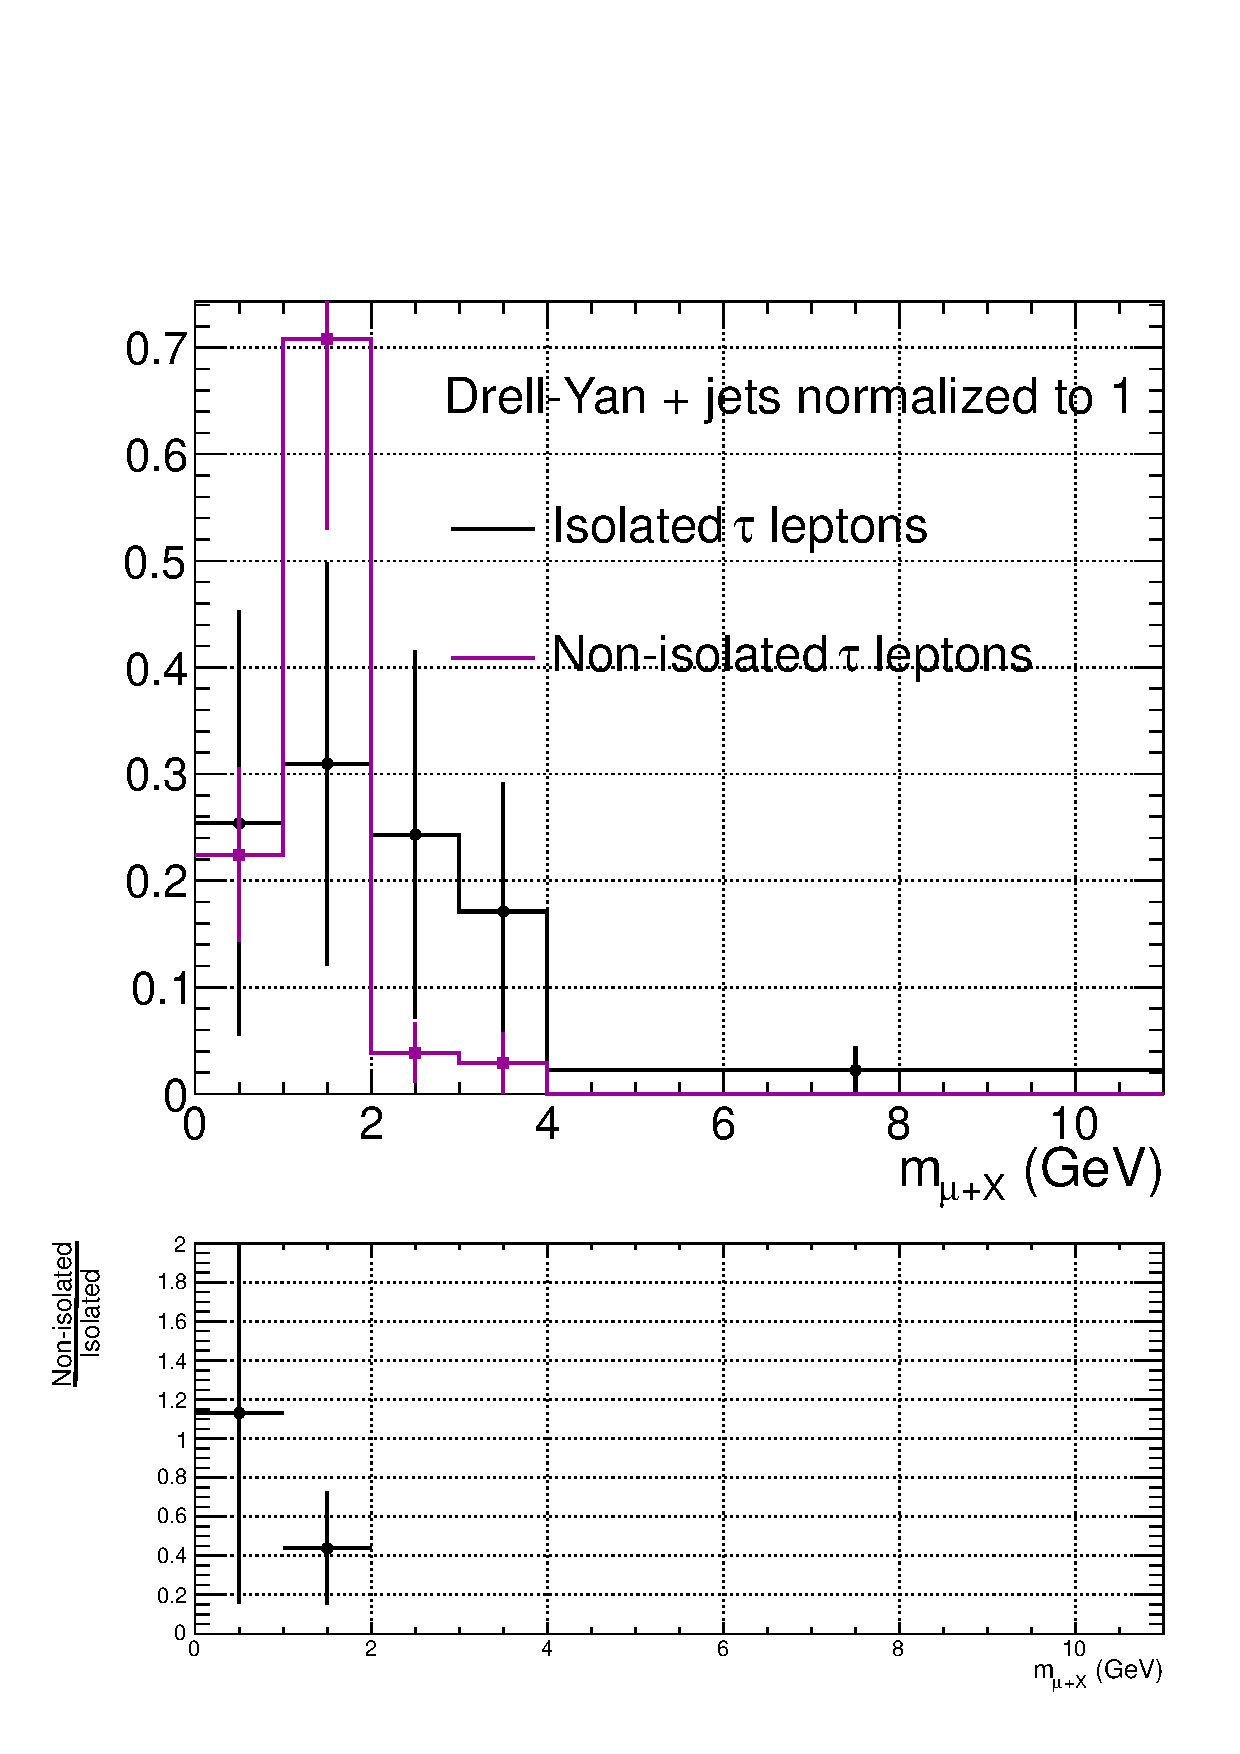
\includegraphics[width=0.8\cmsFigWidth]{figures/isoVsNonIsoTaus_DY_highMT_v87}
    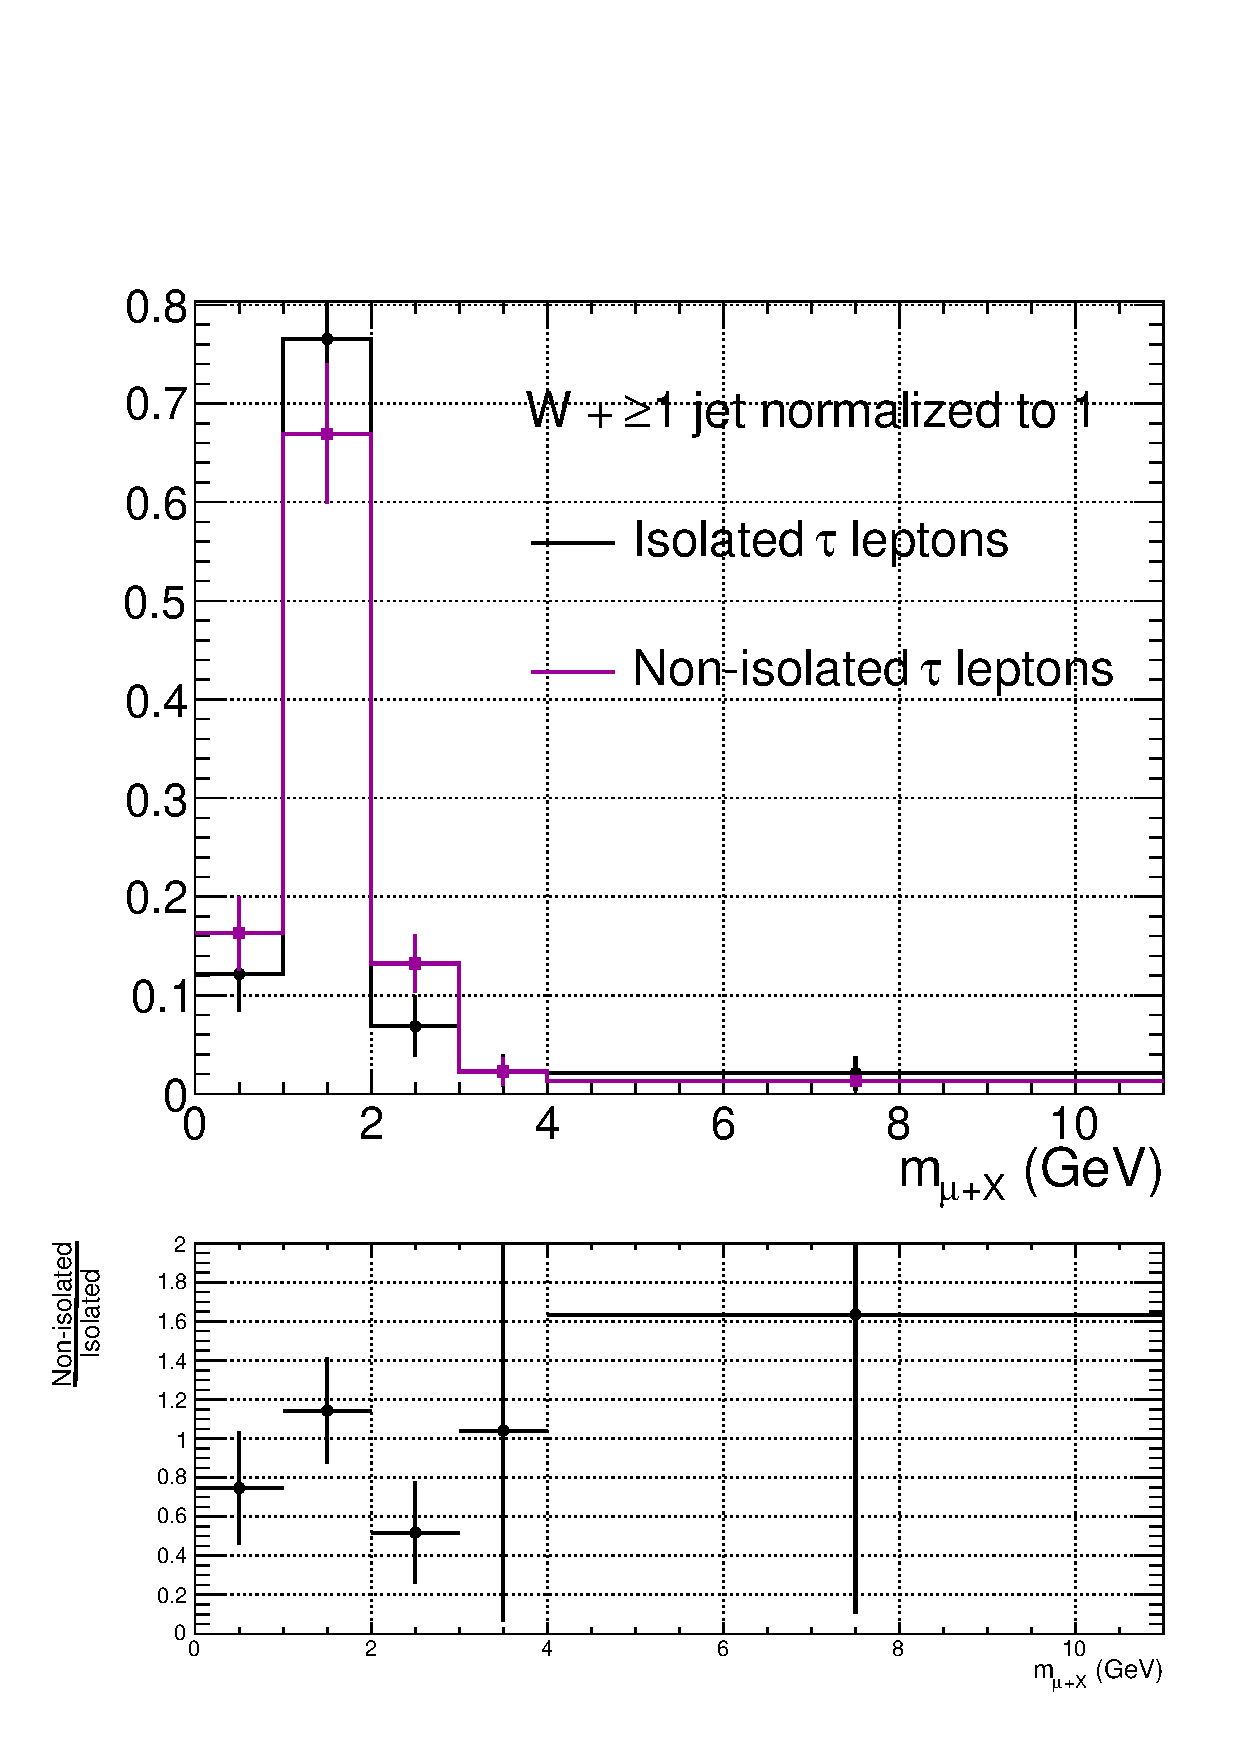
\includegraphics[width=0.8\cmsFigWidth]{figures/isoVsNonIsoTaus_WNJets_highMT_v87}
    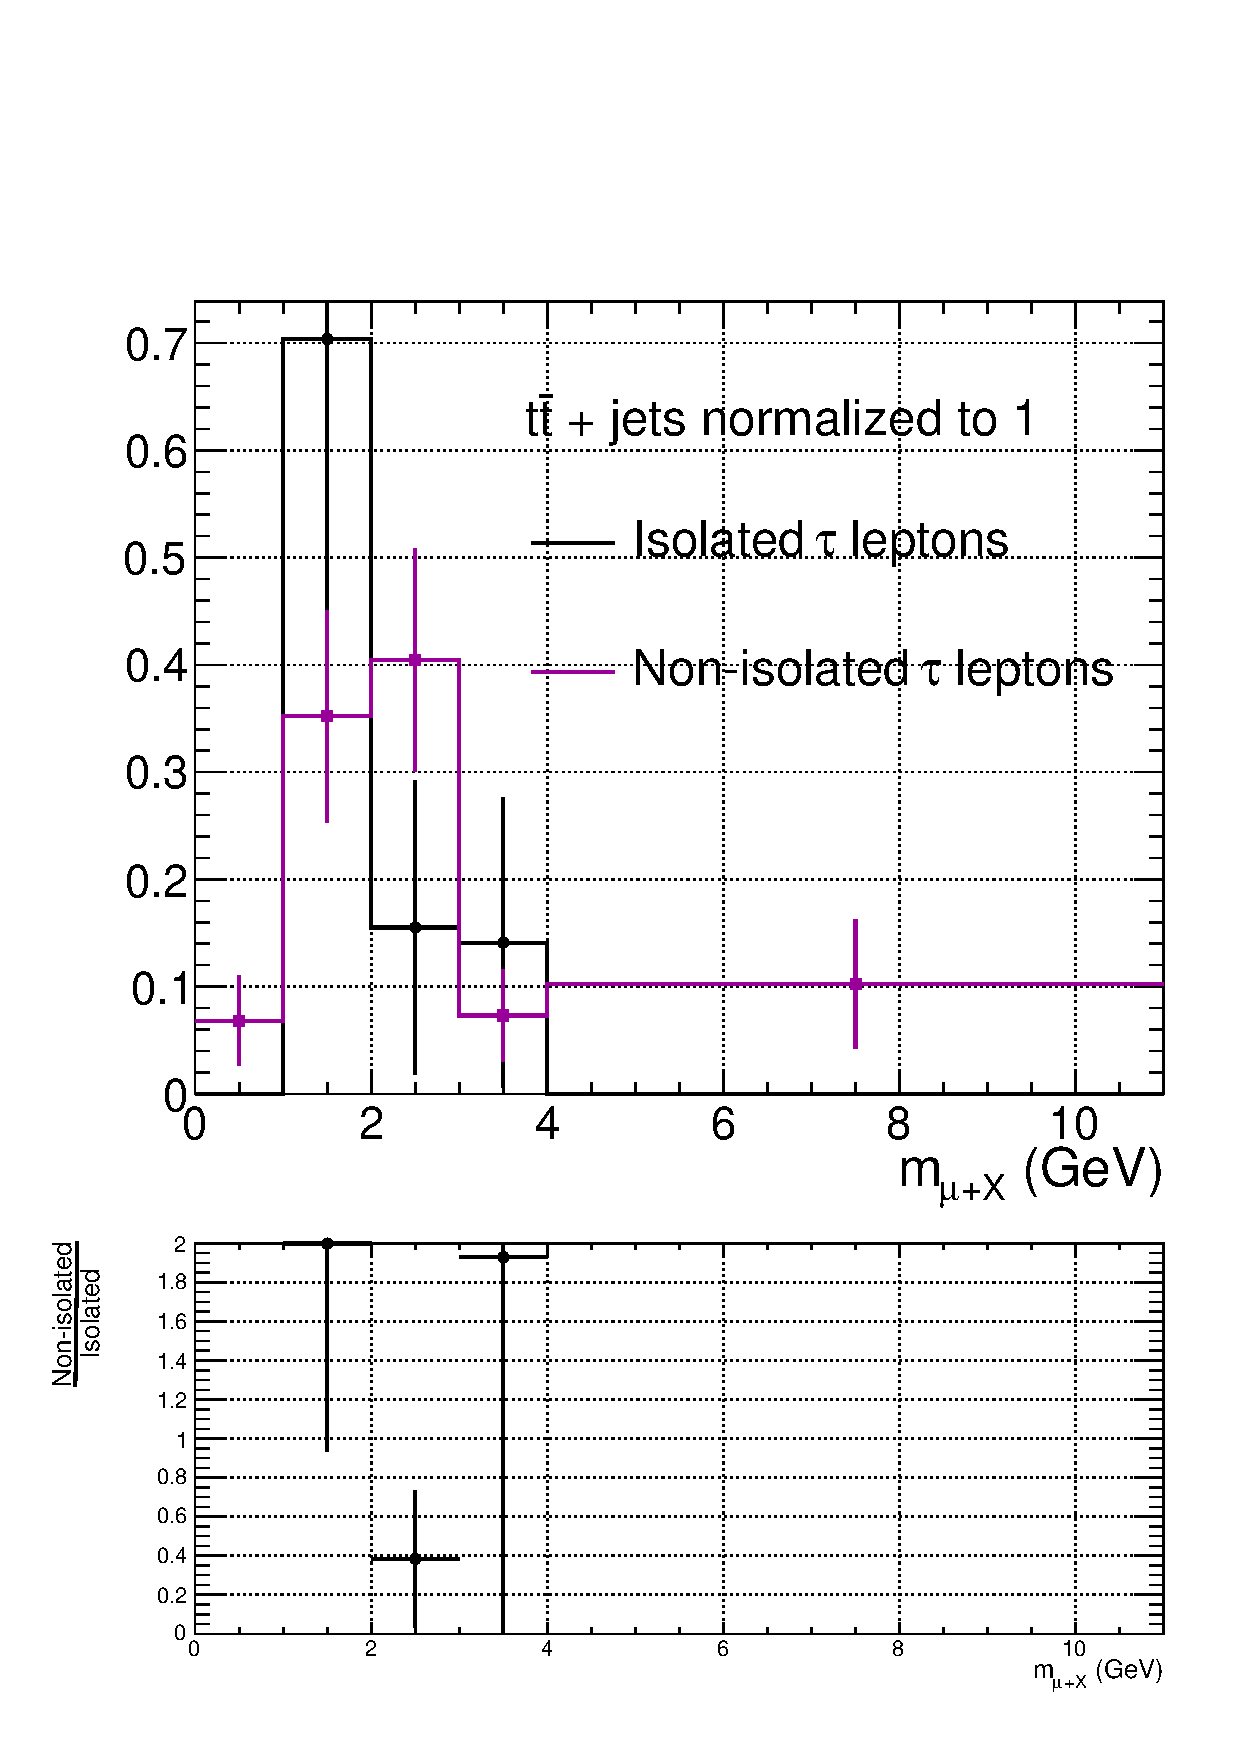
\includegraphics[width=0.8\cmsFigWidth]{figures/isoVsNonIsoTaus_TTJets_highMT_v87}
    \caption{$m_{\mu+\text{had}}$ distributions in the high-$M_{\text{T}}$ bin, normalized to one, for MC events passing the search region selection (black) and the jet fake control region selection (purple).  The small plots beneath the main plots show the ratio of the control region distribution to the search region distribution.  Errors are statistical only.  (\cmsLeft) Drell-Yan.  (Middle) $W$ + $\ge$1 jet.  (\cmsRight) $t\bar{t}$.}
    \label{fig:MC-regA-vs-regB-main-highMT}
  \end{center}
\end{figure}

\begin{figure}[hbtp]
  \begin{center}
    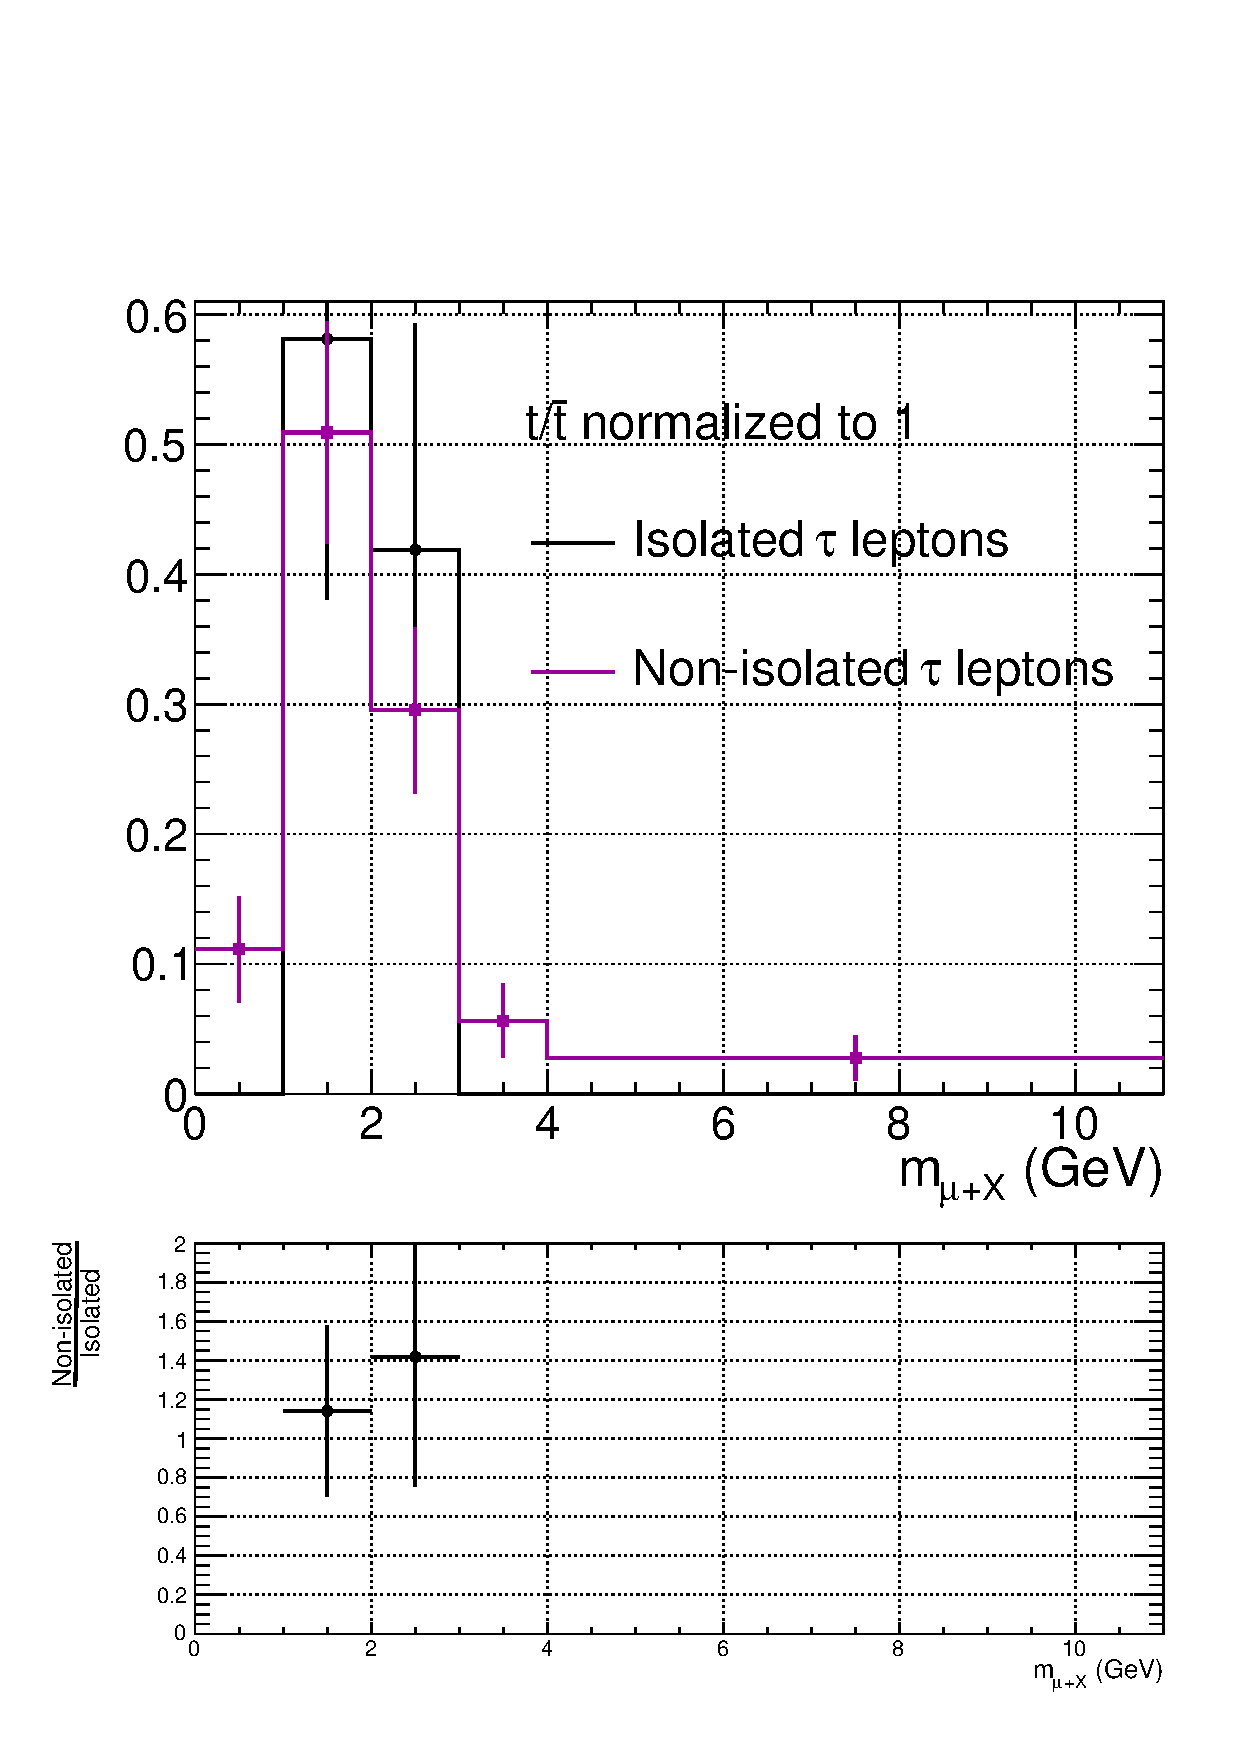
\includegraphics[width=0.6\cmsFigWidth]{figures/isoVsNonIsoTaus_SingleTop_highMT_v87}
    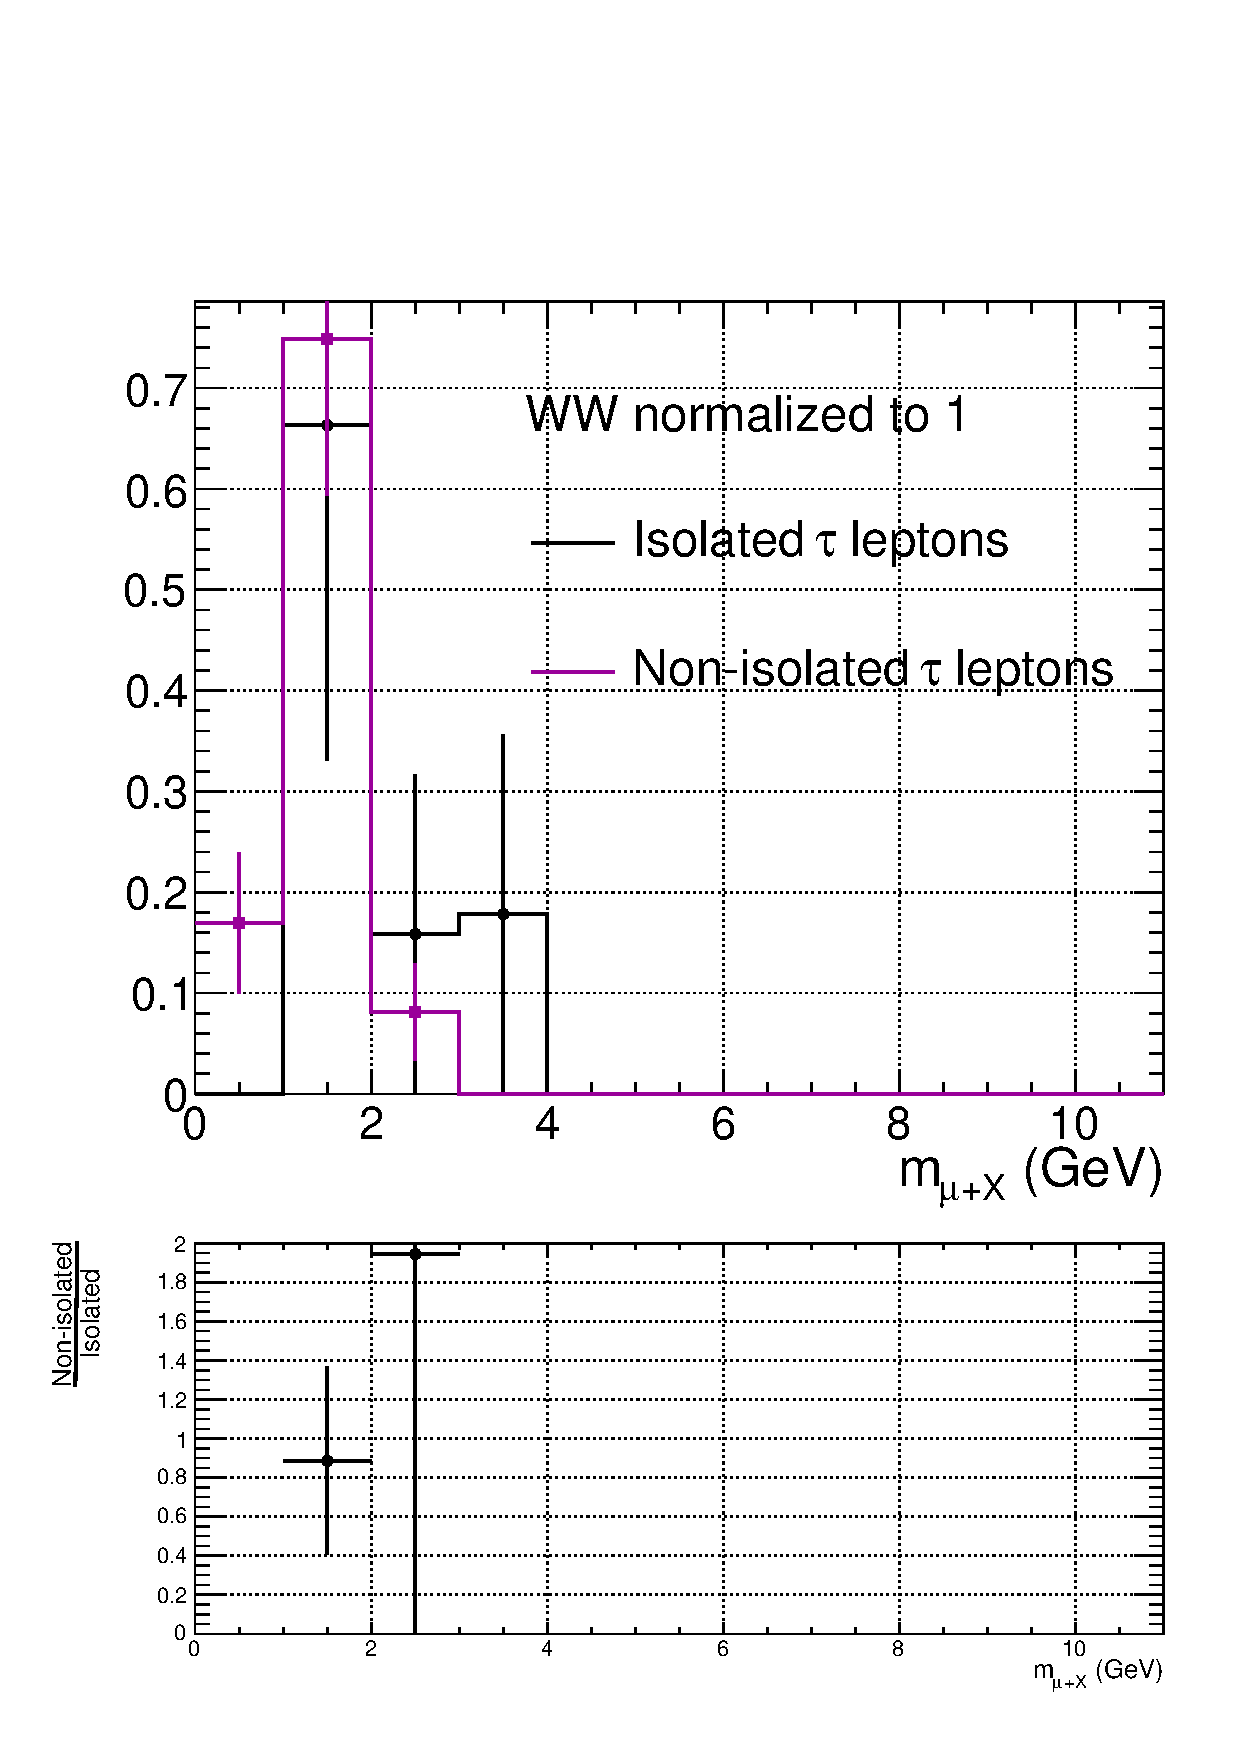
\includegraphics[width=0.6\cmsFigWidth]{figures/isoVsNonIsoTaus_WW_highMT_v87}
    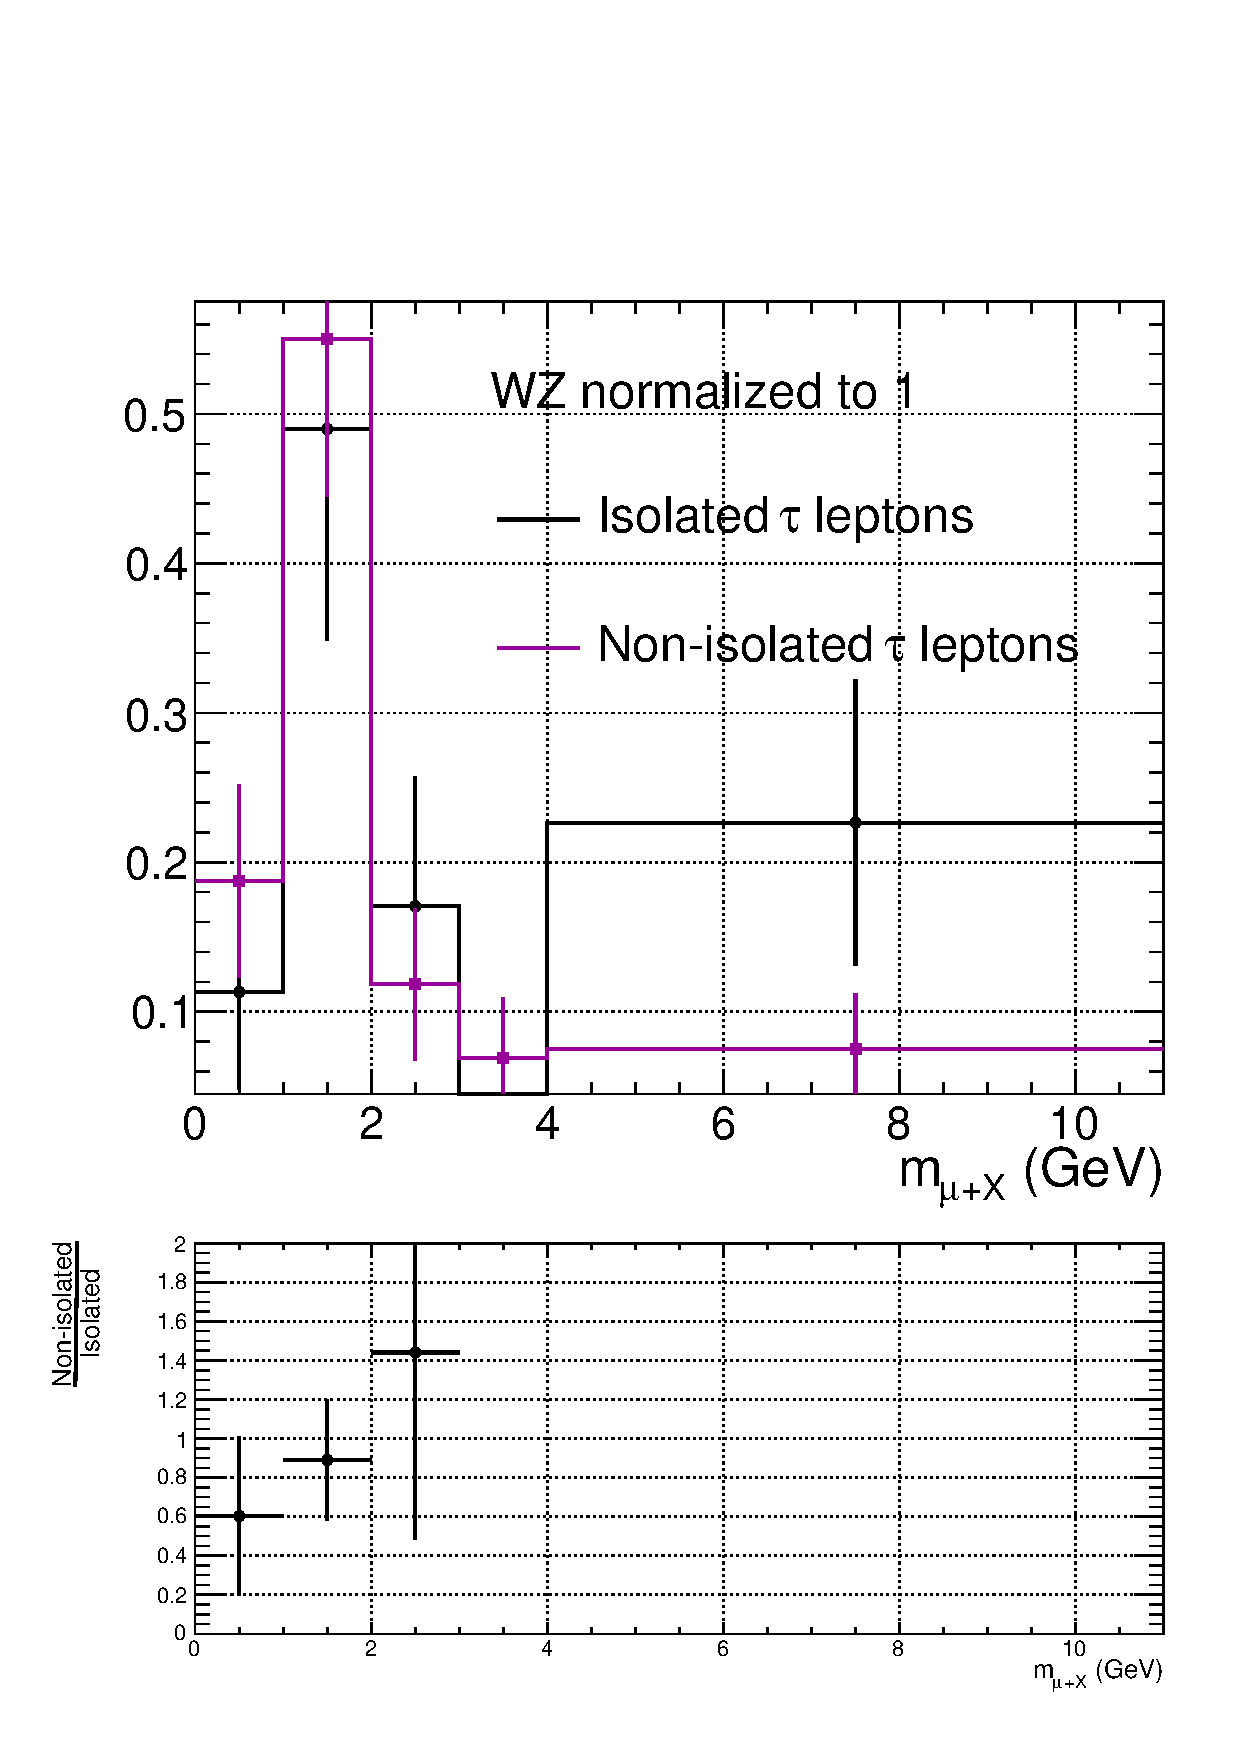
\includegraphics[width=0.6\cmsFigWidth]{figures/isoVsNonIsoTaus_WZ_highMT_v87}
    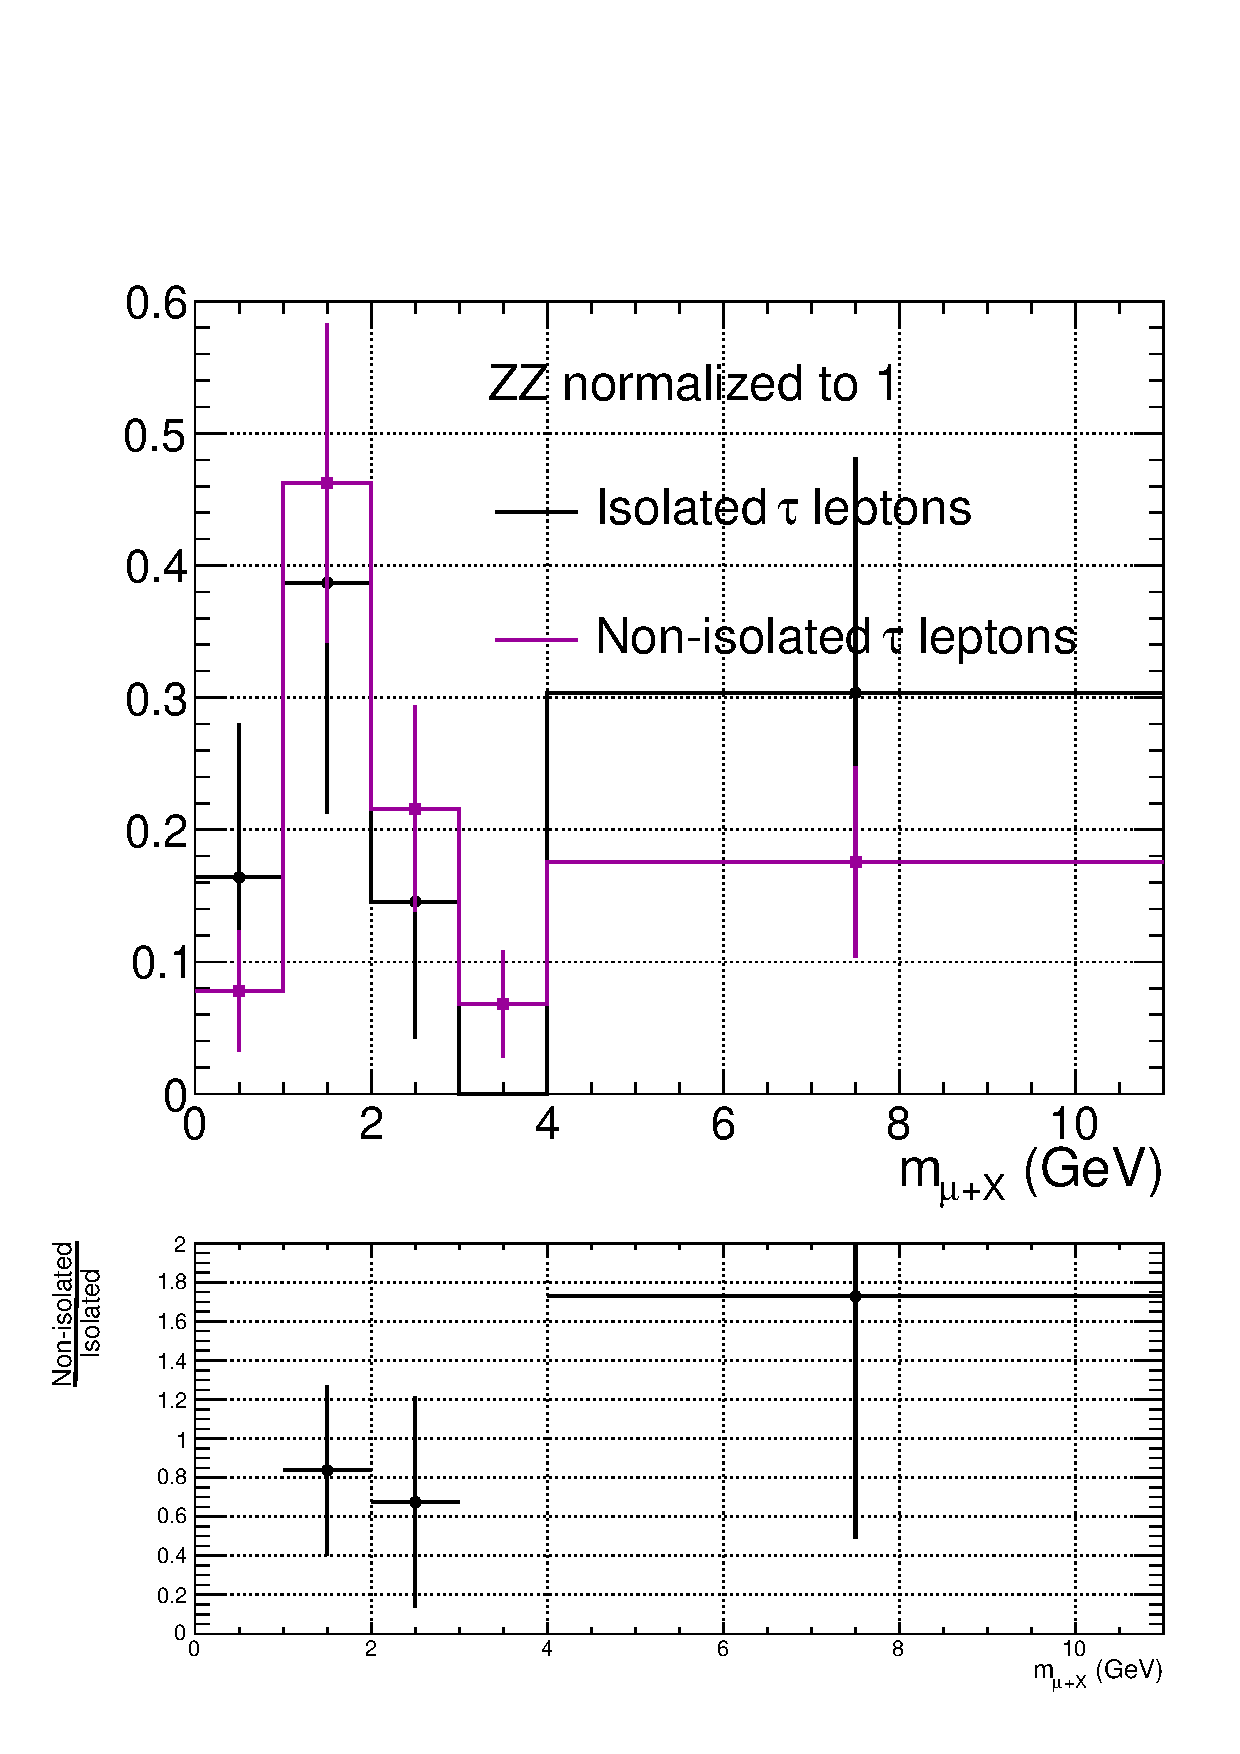
\includegraphics[width=0.6\cmsFigWidth]{figures/isoVsNonIsoTaus_ZZ_highMT_v87}
    \caption{$m_{\mu+\text{had}}$ distributions in the high-$M_{\text{T}}$ bin, normalized to one, for MC events passing the search region selection (black) and the jet fake control region selection (purple).  The small plots beneath the main plots show the ratio of the control region distribution to the search region distribution.  Errors are statistical only.  (\cmsLeft) Single top.  (Middle \cmsLeft) WW.  (Middle \cmsRight) WZ.  (\cmsRight) ZZ.}
    \label{fig:MC-regA-vs-regB-secondary-highMT}
  \end{center}
\end{figure}

\begin{figure}[hbtp]
  \begin{center}
    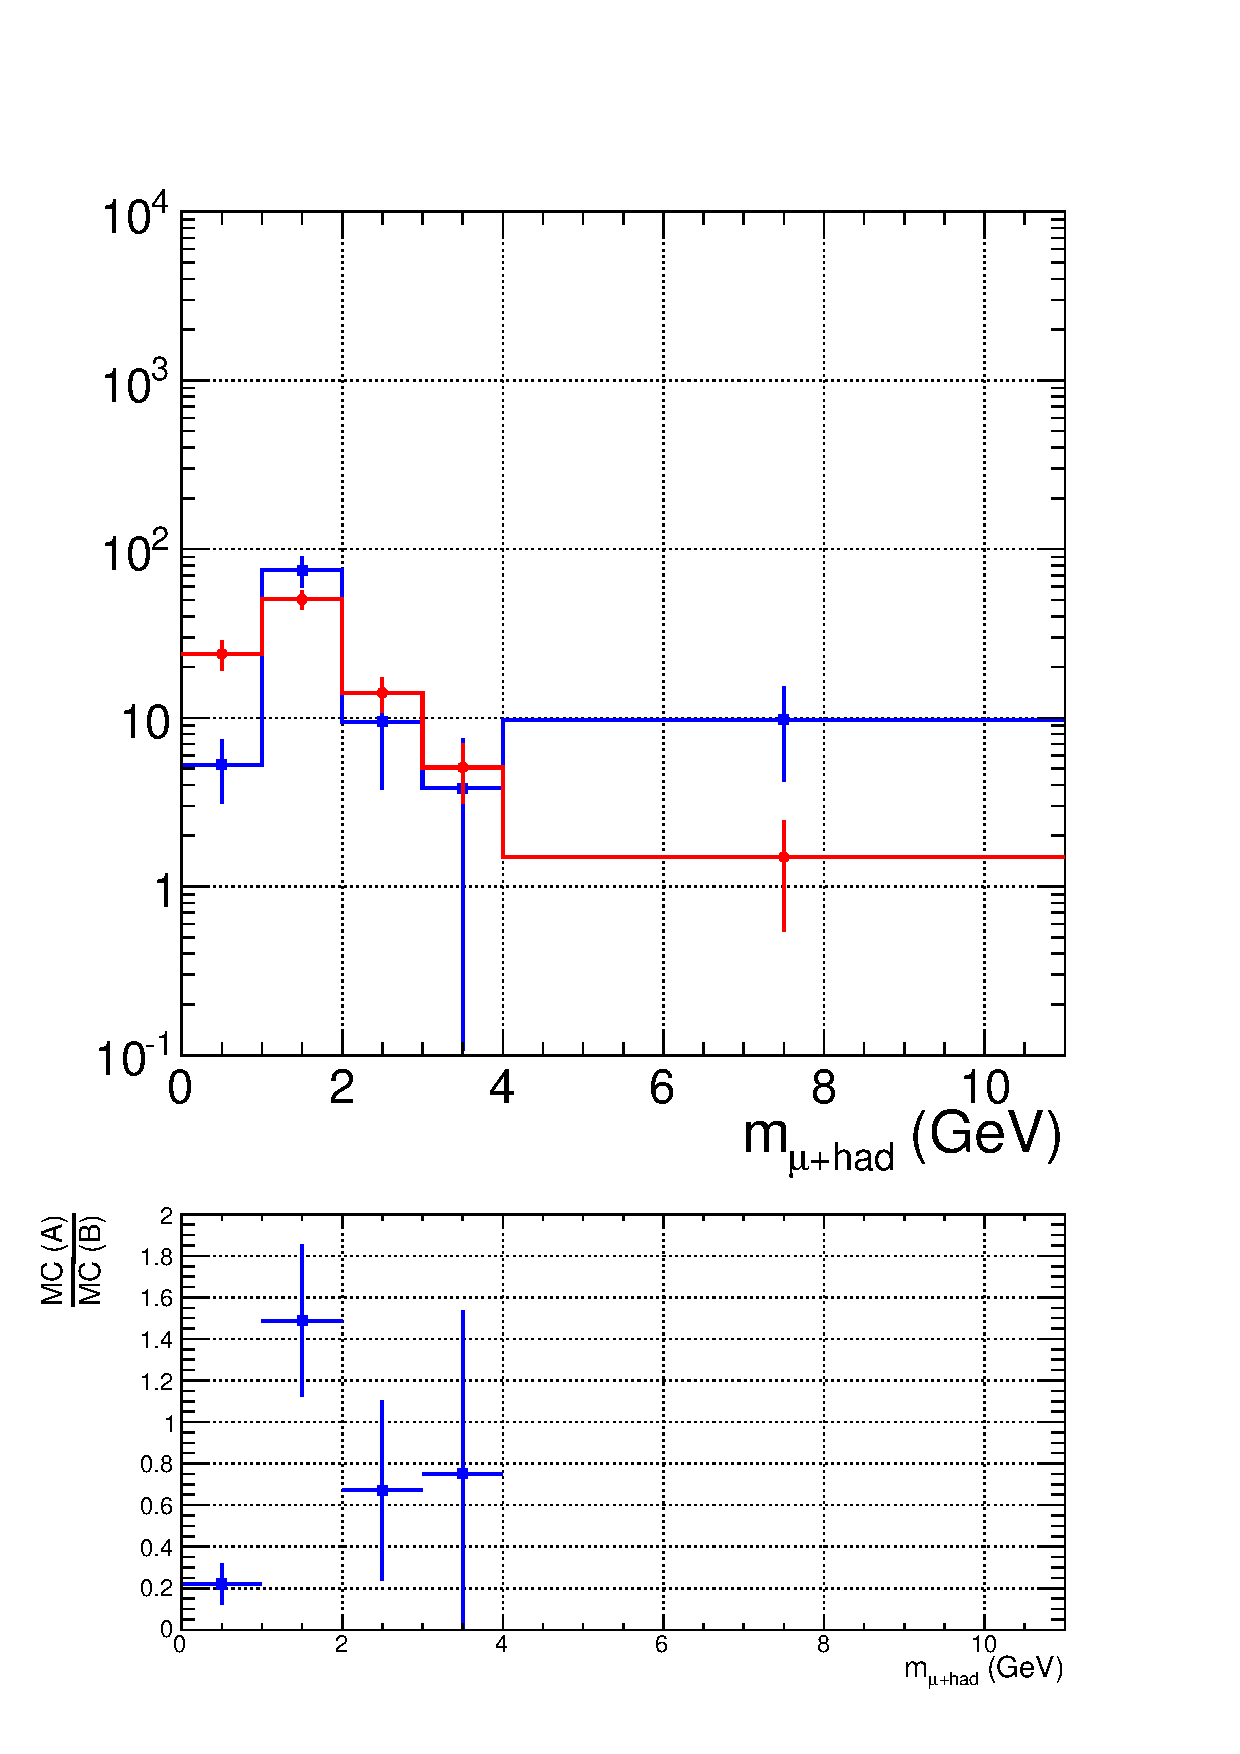
\includegraphics[width=\cmsFigWidth]{figures/MCClosure_lowMT_v87}
    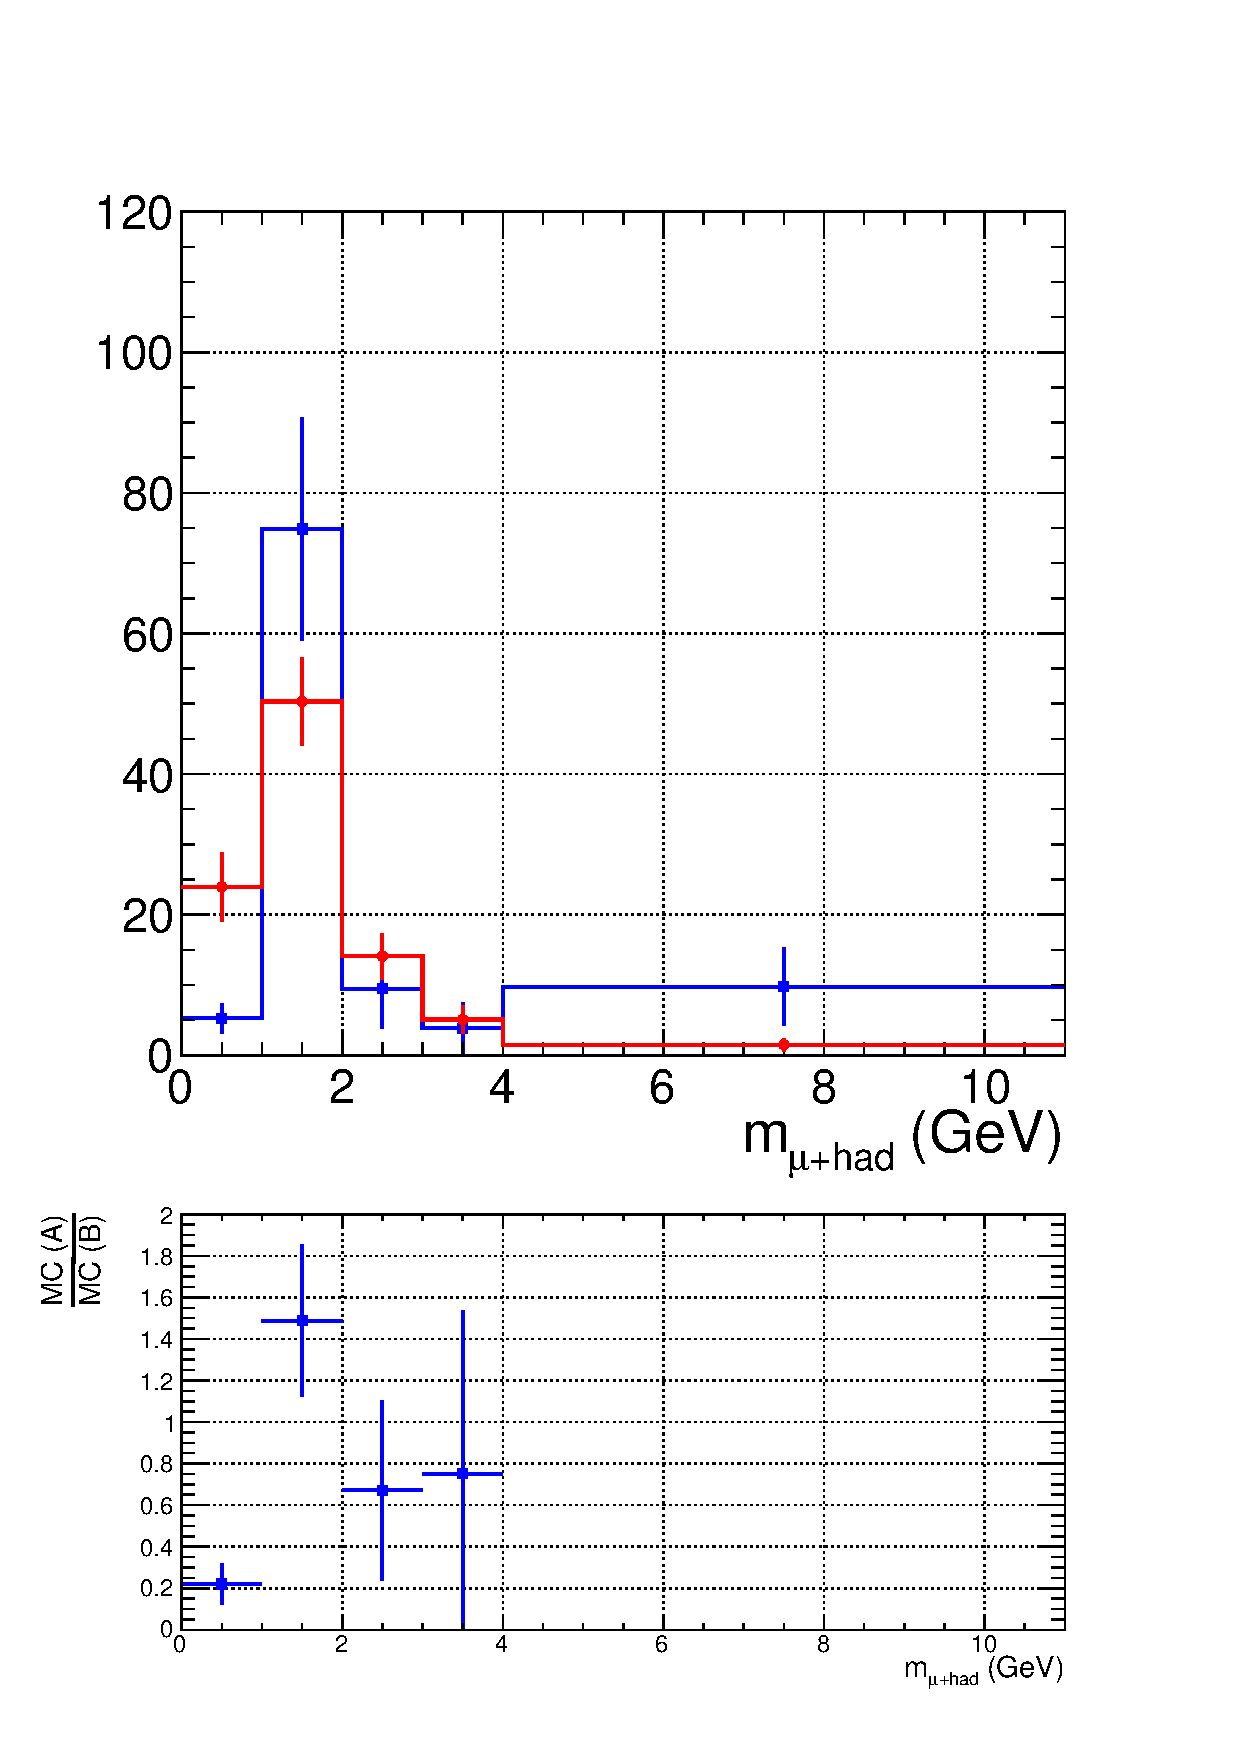
\includegraphics[width=\cmsFigWidth]{figures/MCClosure_linear_lowMT_v87}
    \caption{Comparison of the $m_{\mu+\text{had}}$ distribution for the sum of the simulated backgrounds (all except QCD multi-jets) in the low-$M_{\text{T}}$ bin in the signal region A (blue) with the same distribution in the sideband control region B (red), which is used to model the total background distribution in region A.  The search region distribution is normalized to 19.7 fb$^{-1}$, while the control region distribution is normalized to the area of the search region distribution.  The small plots beneath the main plots show the ratio of the search region distribution to the control region distribution.  Errors are statistical only.  (\cmsLeft) Log scale for y axis.  (\cmsRight) Linear scale for y axis.}
    \label{fig:MC-regA-vs-regB-lowMT}
  \end{center}
\end{figure}

\begin{figure}[hbtp]
  \begin{center}
    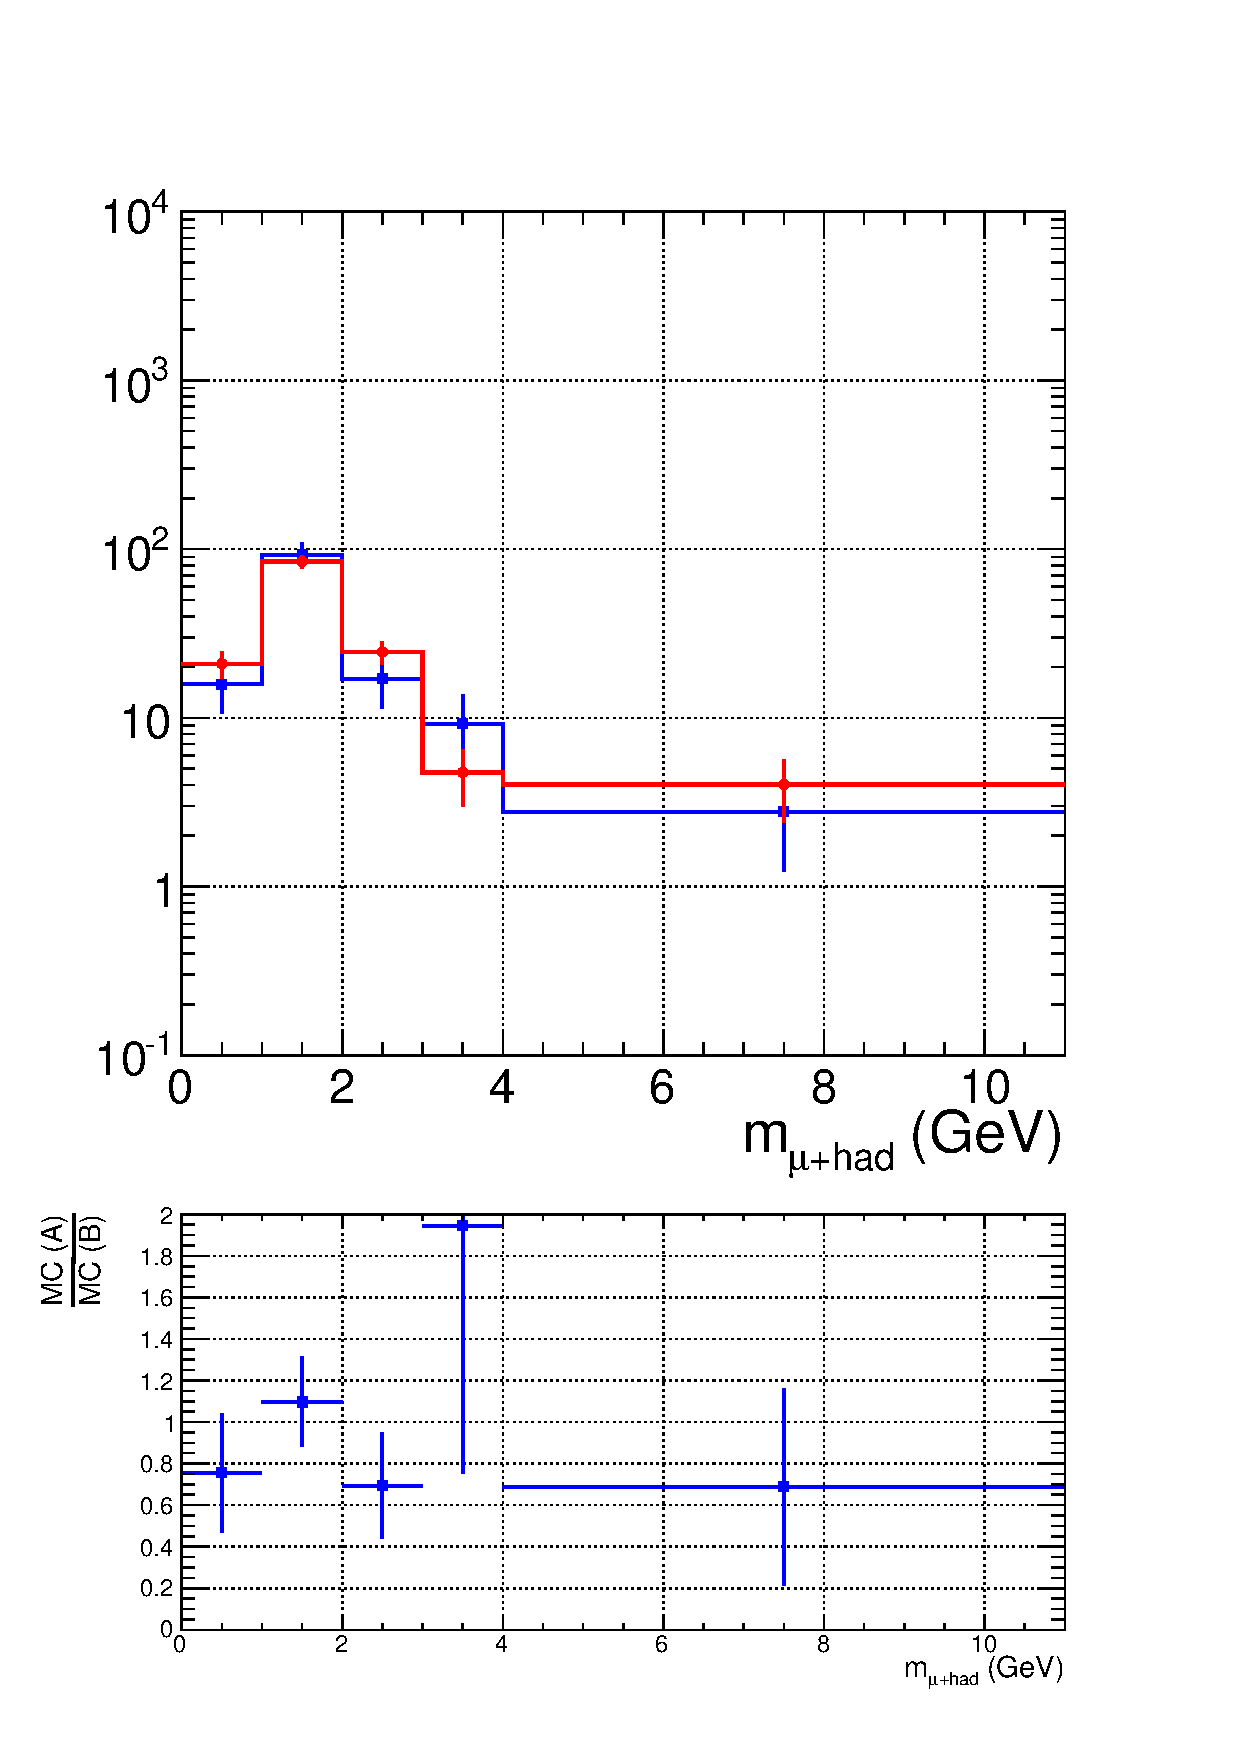
\includegraphics[width=\cmsFigWidth]{figures/MCClosure_highMT_v87}
    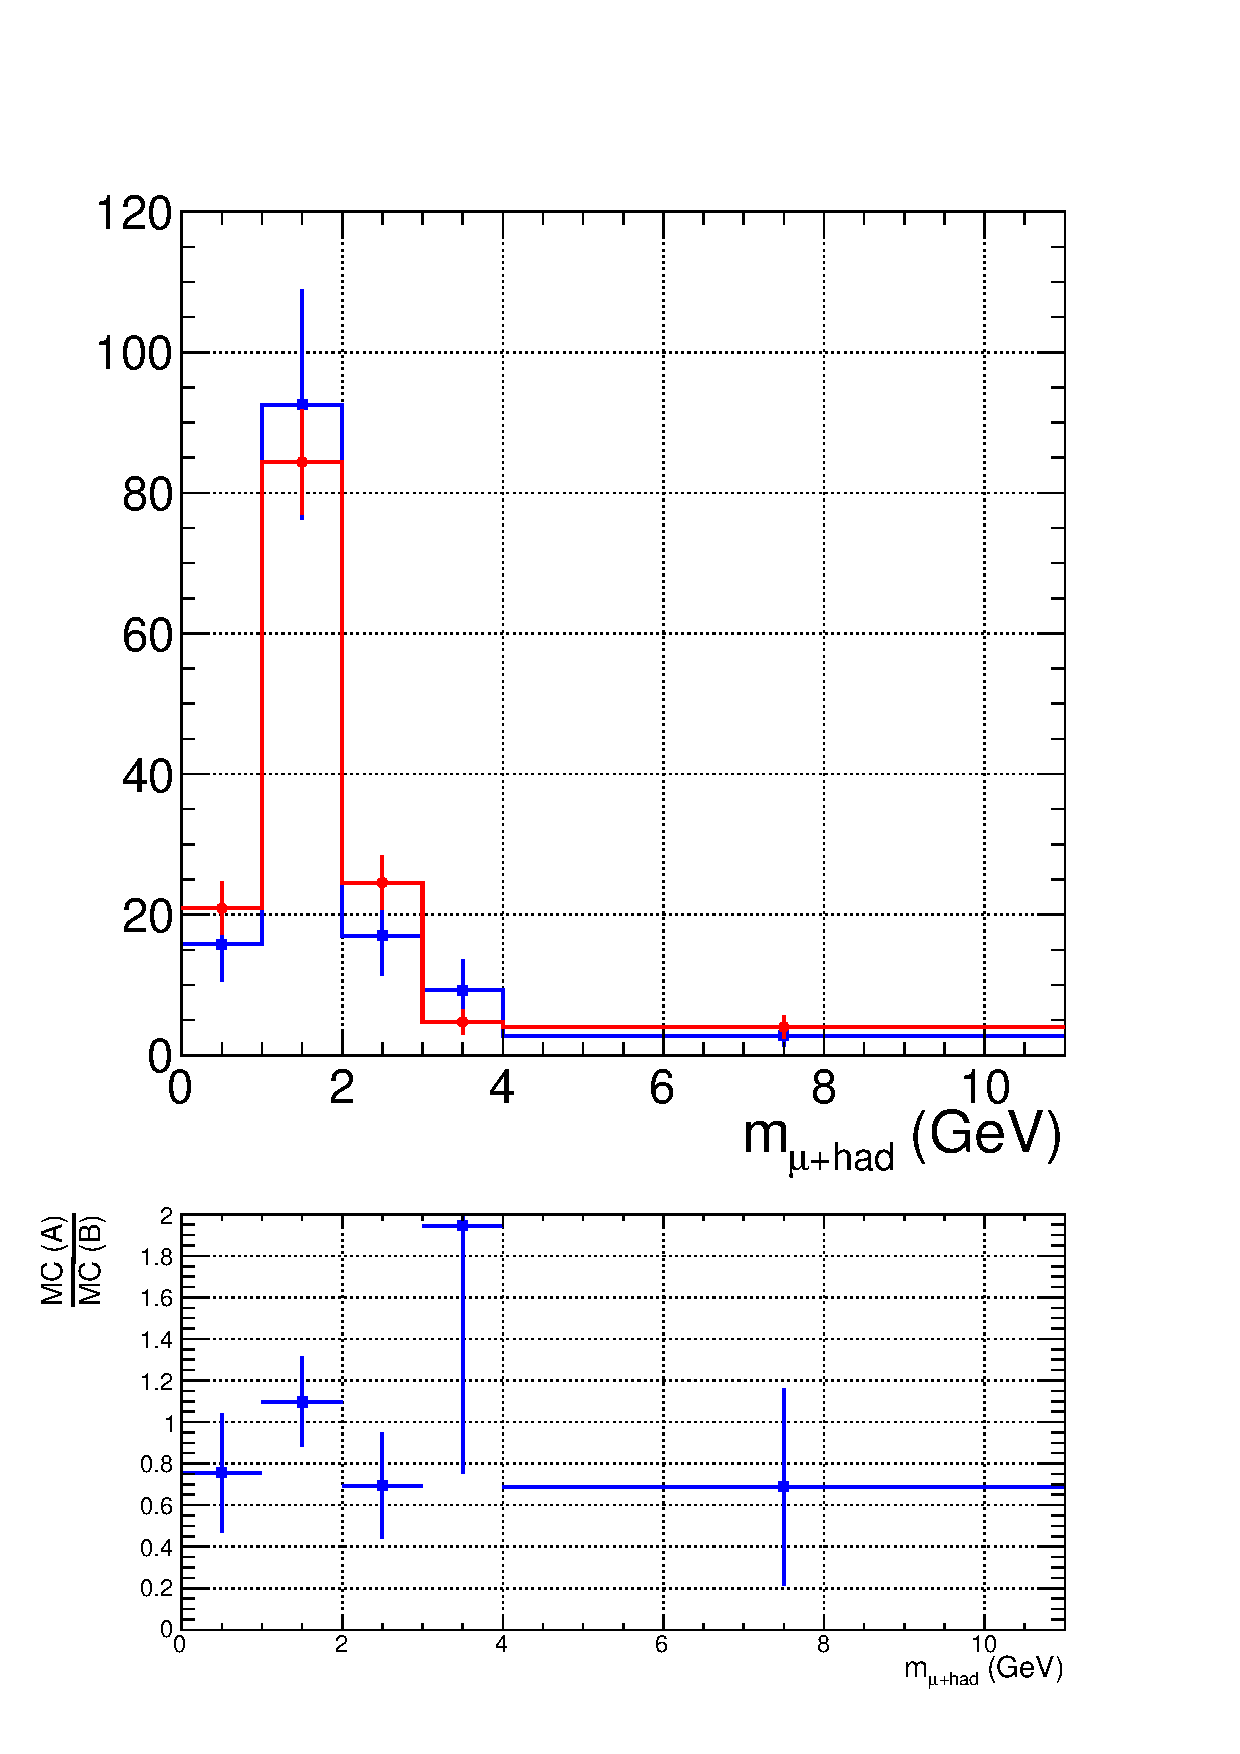
\includegraphics[width=\cmsFigWidth]{figures/MCClosure_linear_highMT_v87}
    \caption{Comparison of the $m_{\mu+\text{had}}$ distribution for the sum of the simulated backgrounds (all except QCD multi-jets) in the low-$M_{\text{T}}$ bin in the signal region A (blue) with the same distribution in the sideband control region B (red), which is used to model the total background distribution in region A.  The search region distribution is normalized to 19.7 fb$^{-1}$, while the control region distribution is normalized to the area of the search region distribution.  The small plots beneath the main plots show the ratio of the search region distribution to the control region distribution.  Errors are statistical only.  (\cmsLeft) Log scale for y axis.  (\cmsRight) Linear scale for y axis.}
    \label{fig:MC-regA-vs-regB-highMT}
  \end{center}
\end{figure}

In the high-$M_{\text{T}}$ bin, where the main backgrounds are $W$ + jets and $t\bar{t}$, the total $m_{\mu+\text{had}}$ shape from simulation is consistent with the total region B shape within statistical errors separately for the $W$ + jets and $t\bar{t}$ samples (Figs.~\ref{fig:MC-regA-vs-regB-main-highMT} (middle) and~\ref{fig:MC-regA-vs-regB-main-highMT} (\cmsRight)).  In the low-$M_{\text{T}}$ bin, where the main backgrounds are QCD di-jets (no MC simulation available) and Drell-Yan + jets, the consistency between regions A and B separately for each MC sample is not as good.

%Subsection: qcd control regions
\subsection{QCD-enriched control regions in data\label{sec:bkgs-qcd-control}}

Two cross-checks are done to establish that the background from jets with double muon decays or isolated di-muon resonances (``resonances") is negligible.  For these cross checks, two other control samples, defined from the trigger muon isolation sideband (``region C" and ``region D'', cf. Figure~\ref{fig:regionsAB}), are used.  Since the trigger muon is required to be non-isolated, these regions are enriched in QCD di-jets, including heavy flavor jets with leptonic decays.  In the $m_{\mu+\text{had}}$ region around the $J\slash\psi$ mass, $\tau_{\mu}\tau_{\text{had}}$ resonances arise from $J\slash\psi\rightarrow\mu\mu$ decays where one muon fakes a tau.  In the $m_{\mu+\text{had}}$ region around the $\Upsilon$ mass, $\tau_{\mu}\tau_{\text{had}}$ resonances arise from real $\Upsilon\rightarrow\tau_{\mu}\tau_{\text{had}}$ decays.  In addition, jets may have two semileptonic decays to muons.  The first cross check, described in Section~\ref{sec:bkgs-resonances}, utilizes a fit around the $J\slash\psi$ mass to extract the $J\slash\psi$ component, while the second, described in Section~\ref{sec:bkgs-3-muon}, uses an independent control sample of three-muon events.

Data control regions C (isolated $\tau_{\mu}\tau_{\text{had}}$, non-isolated trigger muon) and D (non-isolated $\tau_{\mu}\tau_{\text{had}}$, non-isolated trigger muon, cf. Fig.~\ref{fig:regionsAB}) are also used to model the QCD di-jet backgrounds in regions A and B for the purpose of checking whether data with non-isolated taus (D) can accurately model data with isolated taus (C). The QCD shape in region A is taken from region C, defined by the trigger muon isolation sideband of the signal region (cf. Figure~\ref{fig:regionsAB}).  The predicted QCD $\tau_{\mu}\tau_{\text{had}}$ mass distribution in region A, denoted $f_{\text{A}}^{\text{QCD}}(m_{\mu+\text{had}})$, is given by

\begin{equation}
\label{eq:f-A-QCD}
f_{\text{A}}^{\text{QCD}}(m_{\mu+\text{had}}) = R_{\text{A}}^{\text{QCD}}\cdot f_{\text{C}}(m_{\mu+\text{had}})
\end{equation}

where

\begin{equation}
\label{eq:R-A-QCD}
R_{\text{A}}^{\text{QCD}} = [\int_{0}^{3 GeV}(f_{\text{B}}^{\text{data}}(m_{\mu+\text{had}}) - f_{\text{B}}^{\text{MC}}(m_{\mu+\text{had}}))dm_{\mu+\text{had}}]/[\int_{0}^{3 GeV}f_{\text{D}}(m_{\mu+\text{had}})dm_{\mu+\text{had}}]
\end{equation}

and $f_{\text{C}}(m_{\mu+\text{had}})$ is the $\tau_{\mu}\tau_{\text{had}}$ mass distribution in region C data.  In other words, the region C data distribution is normalized by a factor similar to that in Eq.~\ref{eq:R-B-QCD}, except that the integral runs from 0 to 3 GeV instead of 0 to infinity.

This procedure assumes that the QCD $m_{\mu+\text{had}}$ distributions in regions C and D have similar, compatible shapes. Analogously to the shape comparisons in regions A and B for the non-QCD background sources in simulation, a comparison of regions C and D is shown in Figure~\ref{fig:regs-C-vs-D}.  The agreement is reasonable, especially in the low $M_{\text{T}}$ bin for $m_{\mu+\text{had}} \geq$ 2 GeV.

\begin{figure}[hbtp]
  \begin{center}
    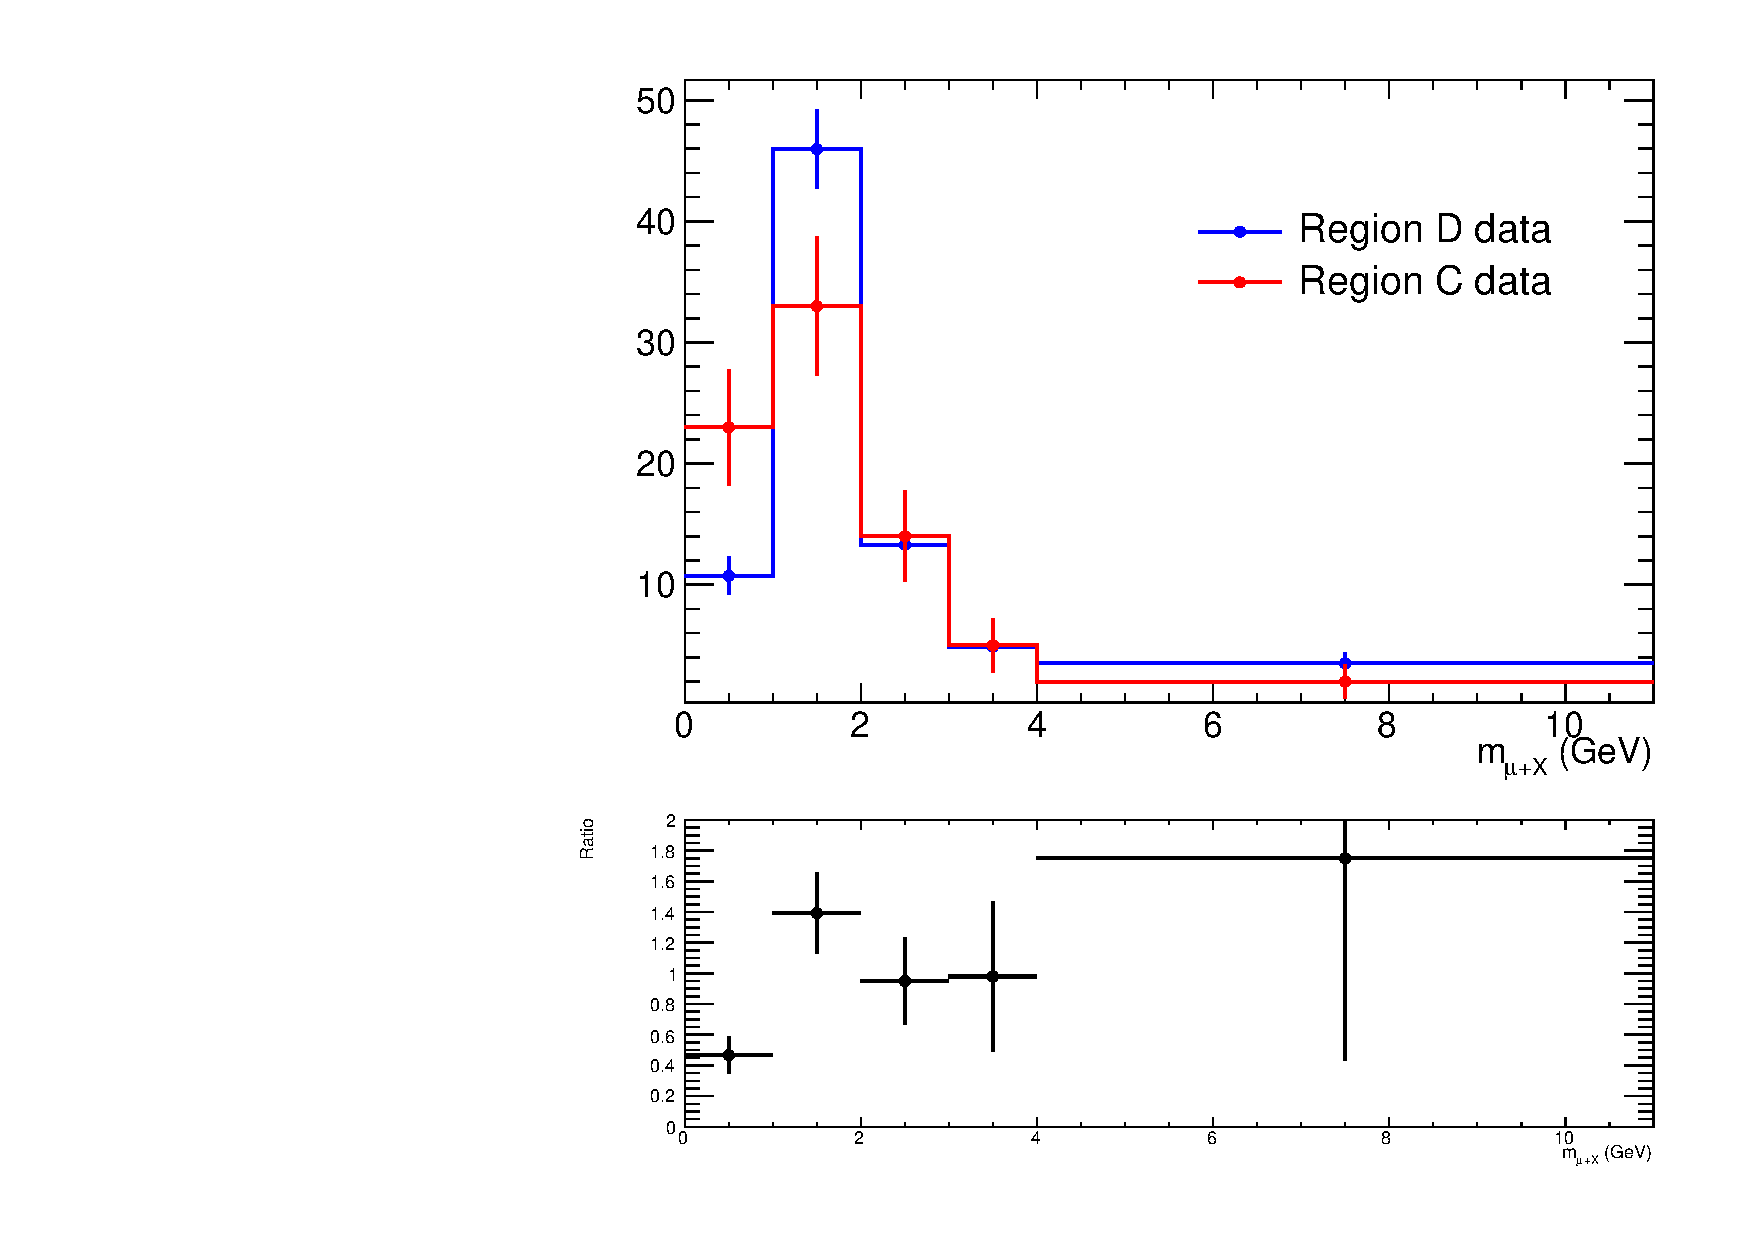
\includegraphics[width=\cmsFigWidth]{figures/regCDataVsRegDData_lowMT}
    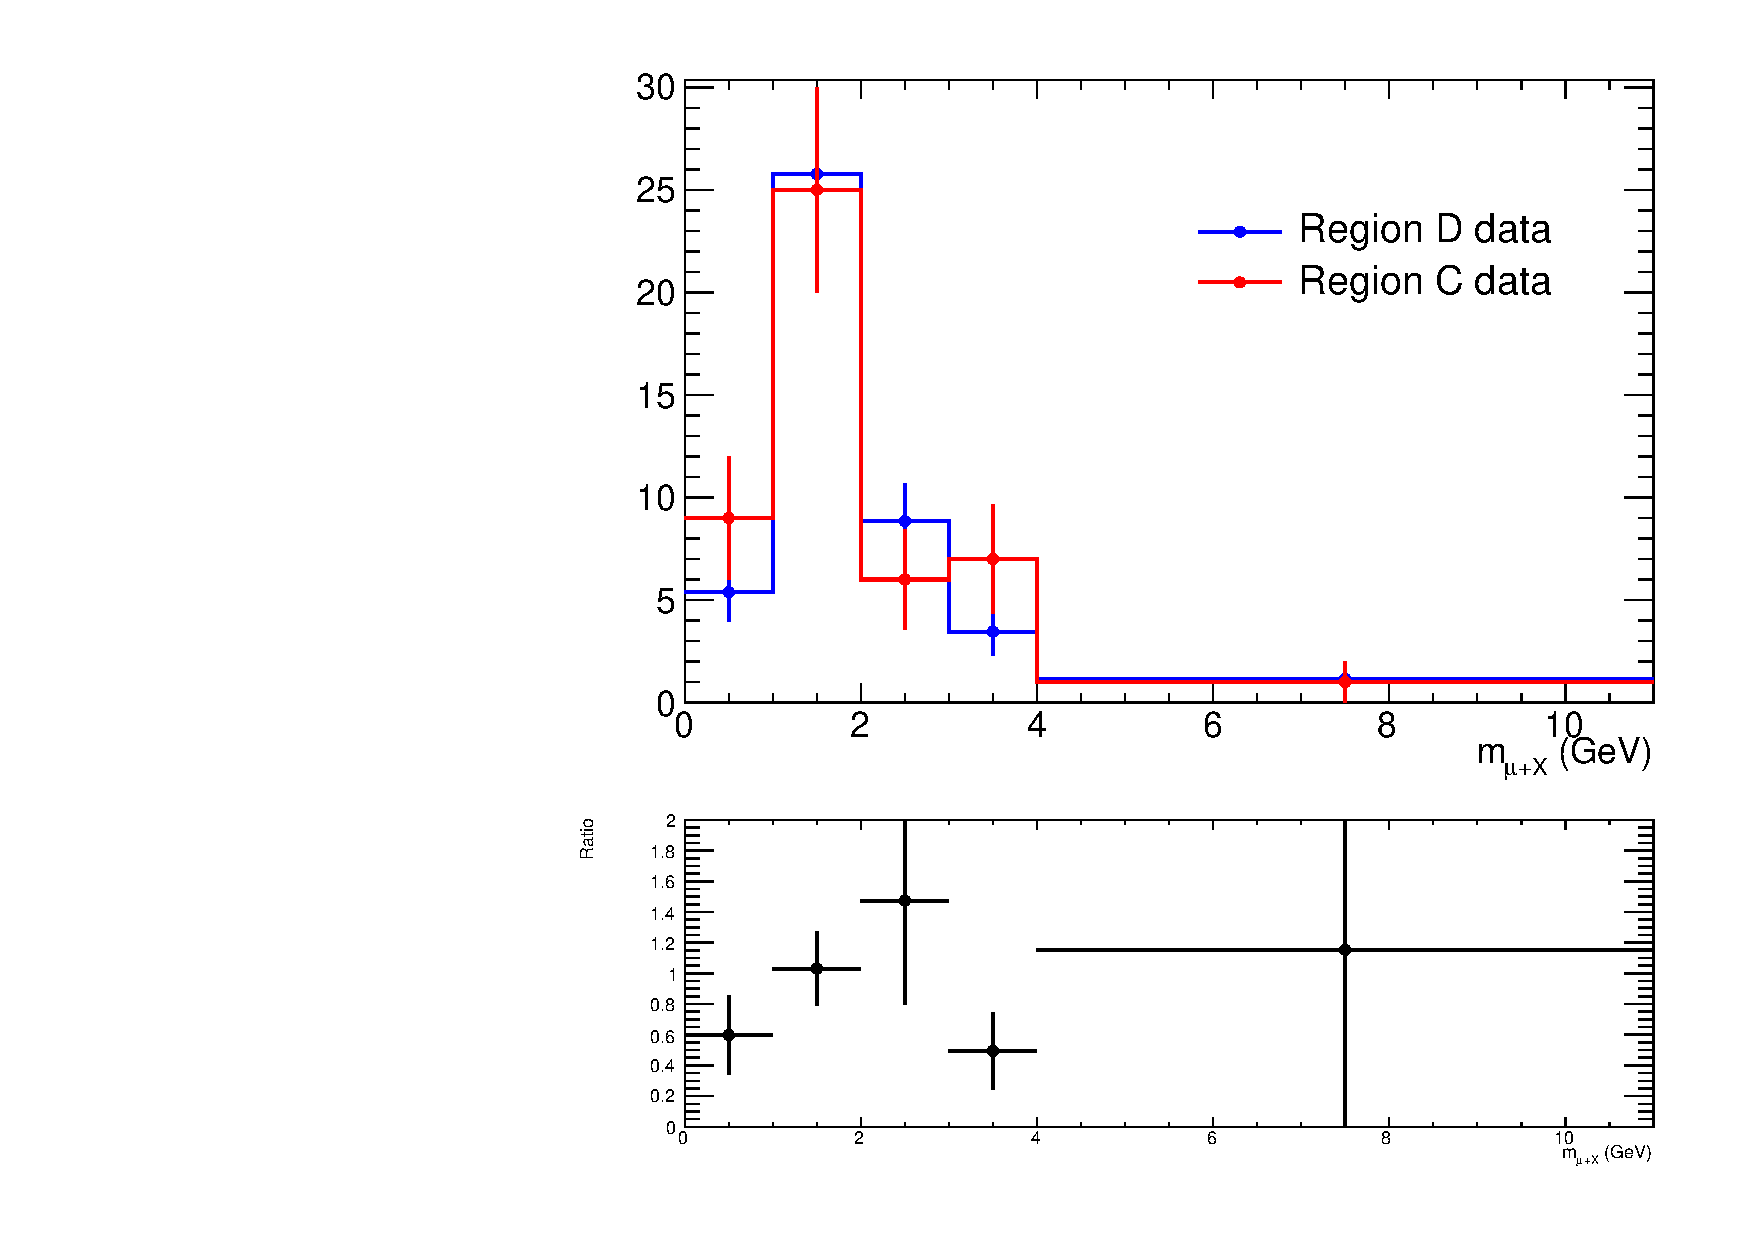
\includegraphics[width=\cmsFigWidth]{figures/regCDataVsRegDData_highMT}
    \caption{$m_{\mu+\text{had}}$ distributions for data events in QCD-enriched regions C and D.  The region D distribution is normalized such that $N_{\text{C}}(m_{\mu+\text{had}} < 3\text{ }GeV)$ = $N_{\text{D}}(m_{\mu+\text{had}} < 3\text{ }GeV)$.  The small plots beneath the main plots show the ratio of the region C distribution to the region D distribution.  Errors are statistical only.  (\cmsLeft) Low $M_{\text{T}}$.  (\cmsRight) High $M_{\text{T}}$.}
    \label{fig:regs-C-vs-D}
  \end{center}
\end{figure}

%The same information is presented in tabular form in Table~\ref{tab:reg-ABCDRatios}.
To supplement the region A/B and C/D comparisons, Table~\ref{tab:reg-ABCDRatios} shows the number of events in the normalization sideband ($m_{\mu+\text{had}}$ $<$ 2 GeV) and search window ($m_{\mu+\text{had}}$ $\ge$ 4 GeV) for individual MC background sources and the data-driven QCD background in Regions A and B after the preselection, as well as the ratio of the number of normalization sideband events to the number of search window events in Regions A and B.

\begin{sidewaystable}
%\begin{table*}[htbH]
\begin{center}
\caption{Number of events after preselection in the normalization sideband ($m_{\mu+\text{had}}$ $<$ 2 GeV) and in the search window ($m_{\mu+\text{had}}$ $\ge$ 4 GeV) for individual MC backgrounds and the data-driven QCD background in Regions A and B, and the ratio of normalization sideband events to search window events.  The MC backgrounds are normalized to 19.7 fb$^{-1}$.  The data-driven QCD background shape for region A(B) comes from region C(D), while the normalization is discussed in Sections~\ref{sec:bkgs-test-MC} and~\ref{sec:bkgs-regB-data-MC}.\label{tab:reg-ABCDRatios}}
\singlespacing
\resizebox{\textwidth}{!}{\begin{tabular}{|l|c|c|c|c|c|c|}
\hline
& \multicolumn{3}{c}{Signal region (A)} & \multicolumn{3}{|c|}{Control region (B)} \\
\hline
$\text{M}_{\text{T}}$ $\le$ 50 GeV & $m_{\mu+\text{had}}$ $<$ 2 GeV & $m_{\mu+\text{had}}$ $\ge$ 4 GeV & $\frac{m_{\mu+\text{had}}\text{ }<\text{ }2\text{ }GeV}{m_{\mu+\text{had}}\text{ }\ge\text{ }4\text{ }GeV}$ & $m_{\mu+\text{had}}$ $<$ 2 GeV & $m_{\mu+\text{had}}$ $\ge$ 4 GeV & $\frac{m_{\mu+\text{had}}\text{ }<\text{ }2\text{ }GeV}{m_{\mu+\text{had}}\text{ }\ge\text{ }4\text{ }GeV}$ \\
\hline
WW & 0.315 $\pm$ 0.18 & 0 & --- & 0.726 $\pm$ 0.3 & 0 & --- \\
ZZ & 0.262 $\pm$ 0.096 & 0.108 $\pm$ 0.062 & 2.42 $\pm$ 1.7 & 0.998 $\pm$ 0.2 & 0.0421 $\pm$ 0.042 & 23.7 $\pm$ 24 \\
WZ & 0.344 $\pm$ 0.15 & 0 & --- & 1.58 $\pm$ 0.35 & 0 & --- \\
W + jets & 41.1 $\pm$ 10 & 0 & --- & 180 $\pm$ 26 & 0.367 $\pm$ 0.37 & 491 $\pm$ 5e+02 \\
Single top & 1.56 $\pm$ 0.8 & 0.278 $\pm$ 0.28 & 5.61 $\pm$ 6.3 & 4.47 $\pm$ 1.3 & 0.373 $\pm$ 0.32 & 12 $\pm$ 11 \\
$t\bar{t}$ & 9.76 $\pm$ 6.1 & 4.1 $\pm$ 4.1 & 2.38 $\pm$ 2.8 & 35.4 $\pm$ 11 & 0 & --- \\
Drell-Yan + jets & 26.8 $\pm$ 11 & 5.25 $\pm$ 3.7 & 5.1 $\pm$ 4.1 & 110 $\pm$ 22 & 5.92 $\pm$ 4.3 & 18.5 $\pm$ 14 \\
QCD (from data) & 24.9 $\pm$ 7 & 0.89 $\pm$ 0.7 & 28 $\pm$ 23 & 117 $\pm$ 30 & 7.23 $\pm$ 2.8 & 16.2 $\pm$ 7.5 \\
Tot. bkg. (MC + data-driven QCD) & 105 $\pm$ 17 & 10.6 $\pm$ 5.6 & 9.88 $\pm$ 5.4 & 450 $\pm$ 46 & 13.9 $\pm$ 5.1 & 32.3 $\pm$ 12 \\
Data & 122 & 7 & 17.4 & 430 & 22 & 19.5 \\
\hline
$\text{M}_{\text{T}}$ $\geq$ 50 GeV & $m_{\mu+\text{had}}$ $<$ 2 GeV & $m_{\mu+\text{had}}$ $\ge$ 4 GeV & $\frac{m_{\mu+\text{had}}\text{ }<\text{ }2\text{ }GeV}{m_{\mu+\text{had}}\text{ }\ge\text{ }4\text{ }GeV}$ & $m_{\mu+\text{had}}$ $<$ 2 GeV & $m_{\mu+\text{had}}$ $\ge$ 4 GeV & $\frac{m_{\mu+\text{had}}\text{ }<\text{ }2\text{ }GeV}{m_{\mu+\text{had}}\text{ }\ge\text{ }4\text{ }GeV}$ \\
\hline
WW & 0.472 $\pm$ 0.24 & 0 & --- & 3.66 $\pm$ 0.68 & 0 & --- \\
ZZ & 0.263 $\pm$ 0.1 & 0.145 $\pm$ 0.085 & 1.82 $\pm$ 1.3 & 0.723 $\pm$ 0.17 & 0.235 $\pm$ 0.097 & 3.08 $\pm$ 1.5 \\
WZ & 1.08 $\pm$ 0.28 & 0.404 $\pm$ 0.17 & 2.66 $\pm$ 1.3 & 2.71 $\pm$ 0.46 & 0.276 $\pm$ 0.14 & 9.85 $\pm$ 5.2 \\
W + jets & 74.6 $\pm$ 14 & 1.76 $\pm$ 1.5 & 42.4 $\pm$ 36 & 409 $\pm$ 39 & 6.29 $\pm$ 2.8 & 65 $\pm$ 29 \\
Single top & 2.5 $\pm$ 0.86 & 0 & --- & 15.5 $\pm$ 2.4 & 0.69 $\pm$ 0.43 & 22.5 $\pm$ 15 \\
$t\bar{t}$ & 17.7 $\pm$ 8 & 0 & --- & 59.9 $\pm$ 15 & 14.6 $\pm$ 8.6 & 4.11 $\pm$ 2.6 \\
Drell-Yan + jets & 11.7 $\pm$ 5.7 & 0.463 $\pm$ 0.46 & 25.4 $\pm$ 28 & 85.2 $\pm$ 18 & 0 & --- \\
QCD (from data) & 16.7 $\pm$ 15 & 0.49 $\pm$ 0.74 & 34 $\pm$ 60 & 56.5 $\pm$ 36 & 2.09 $\pm$ 2 & 27 $\pm$ 31 \\
Tot. bkg. (MC + data-driven QCD) & 125 $\pm$ 23 & 3.26 $\pm$ 1.7 & 38.3 $\pm$ 21 & 633 $\pm$ 59 & 24.1 $\pm$ 9.2 & 26.2 $\pm$ 10 \\
Data & 166 & 14 & 11.9 & 577 & 20 & 28.9 \\
\hline
\end{tabular}}
\end{center}
%\end{table*}
\end{sidewaystable}

%Subsection: understanding bkg
\subsection{Understanding background composition in jet fake control region (B)\label{sec:bkgs-regB-data-MC}}

In order to understand and have an independent validation of the background composition in the jet fake control region (B), comparisons of data and total non-QCD backgrounds from MC simulation are made for a number of different distributions characterizing region B.  The individual MC background distributions are normalized to the data luminosity of 19.7 fb$^{-1}$ using the cross sections given in Table~\ref{tab:MCBkg}, and event weights are applied to account for the different pileup distributions in data and MC according to the procedure described in Ref.~\cite{PU-Twiki}.  The available QCD MC does not provide enough events passing the control region selection to have any statistical power, so the QCD contribution is taken instead from the QCD-enriched control region in data defined by the trigger muon isolation sideband (``region D'', cf. Figure~\ref{fig:regionsAB}) of the jet fake control region.  The predicted QCD $\tau_{\mu}\tau_{\text{had}}$ mass distribution in region B, denoted $f_{\text{B}}^{\text{QCD}}(m_{\mu+\text{had}})$, is given by

\begin{equation}
\label{eq:f-B-QCD}
f_{\text{B}}^{\text{QCD}}(m_{\mu+\text{had}}) = R_{\text{B}}^{\text{QCD}}\cdot f_{\text{D}}(m_{\mu+\text{had}})
\end{equation}

where

\begin{equation}
\label{eq:R-B-QCD}
R_{\text{B}}^{\text{QCD}} = [\int_{0}^{\infty}(f_{\text{B}}^{\text{data}}(m_{\mu+\text{had}}) - f_{\text{B}}^{\text{MC}}(m_{\mu+\text{had}}))dm_{\mu+\text{had}}]/[\int_{0}^{\infty}f_{\text{D}}(m_{\mu+\text{had}})dm_{\mu+\text{had}}]
\end{equation}

$f_{\text{D}}(m_{\mu+\text{had}})$ is the $\tau_{\mu}\tau_{\text{had}}$ mass distribution in region D data, $f_{\text{B}}^{\text{data}}(m_{\mu+\text{had}})$ is the $\tau_{\mu}\tau_{\text{had}}$ mass distribution in region B data, and $f_{\text{B}}^{\text{MC}}(m_{\mu+\text{had}})$ is the $\tau_{\mu}\tau_{\text{had}}$ mass distribution in region B MC.  In other words, the region D data distribution is normalized to the number of data events minus the sum of MC events in region B, where the MC sum is normalized to 19.7 fb$^{-1}$.  Figure~\ref{fig:QCDComparisonBD} shows the comparison of $m_{\mu+{\text{had}}}$ shapes between region D data and region B data minus total non-QCD background from simulation, which are generally consistent with each other within statistical errors.

\begin{figure}[hbtp]
  \begin{center}
    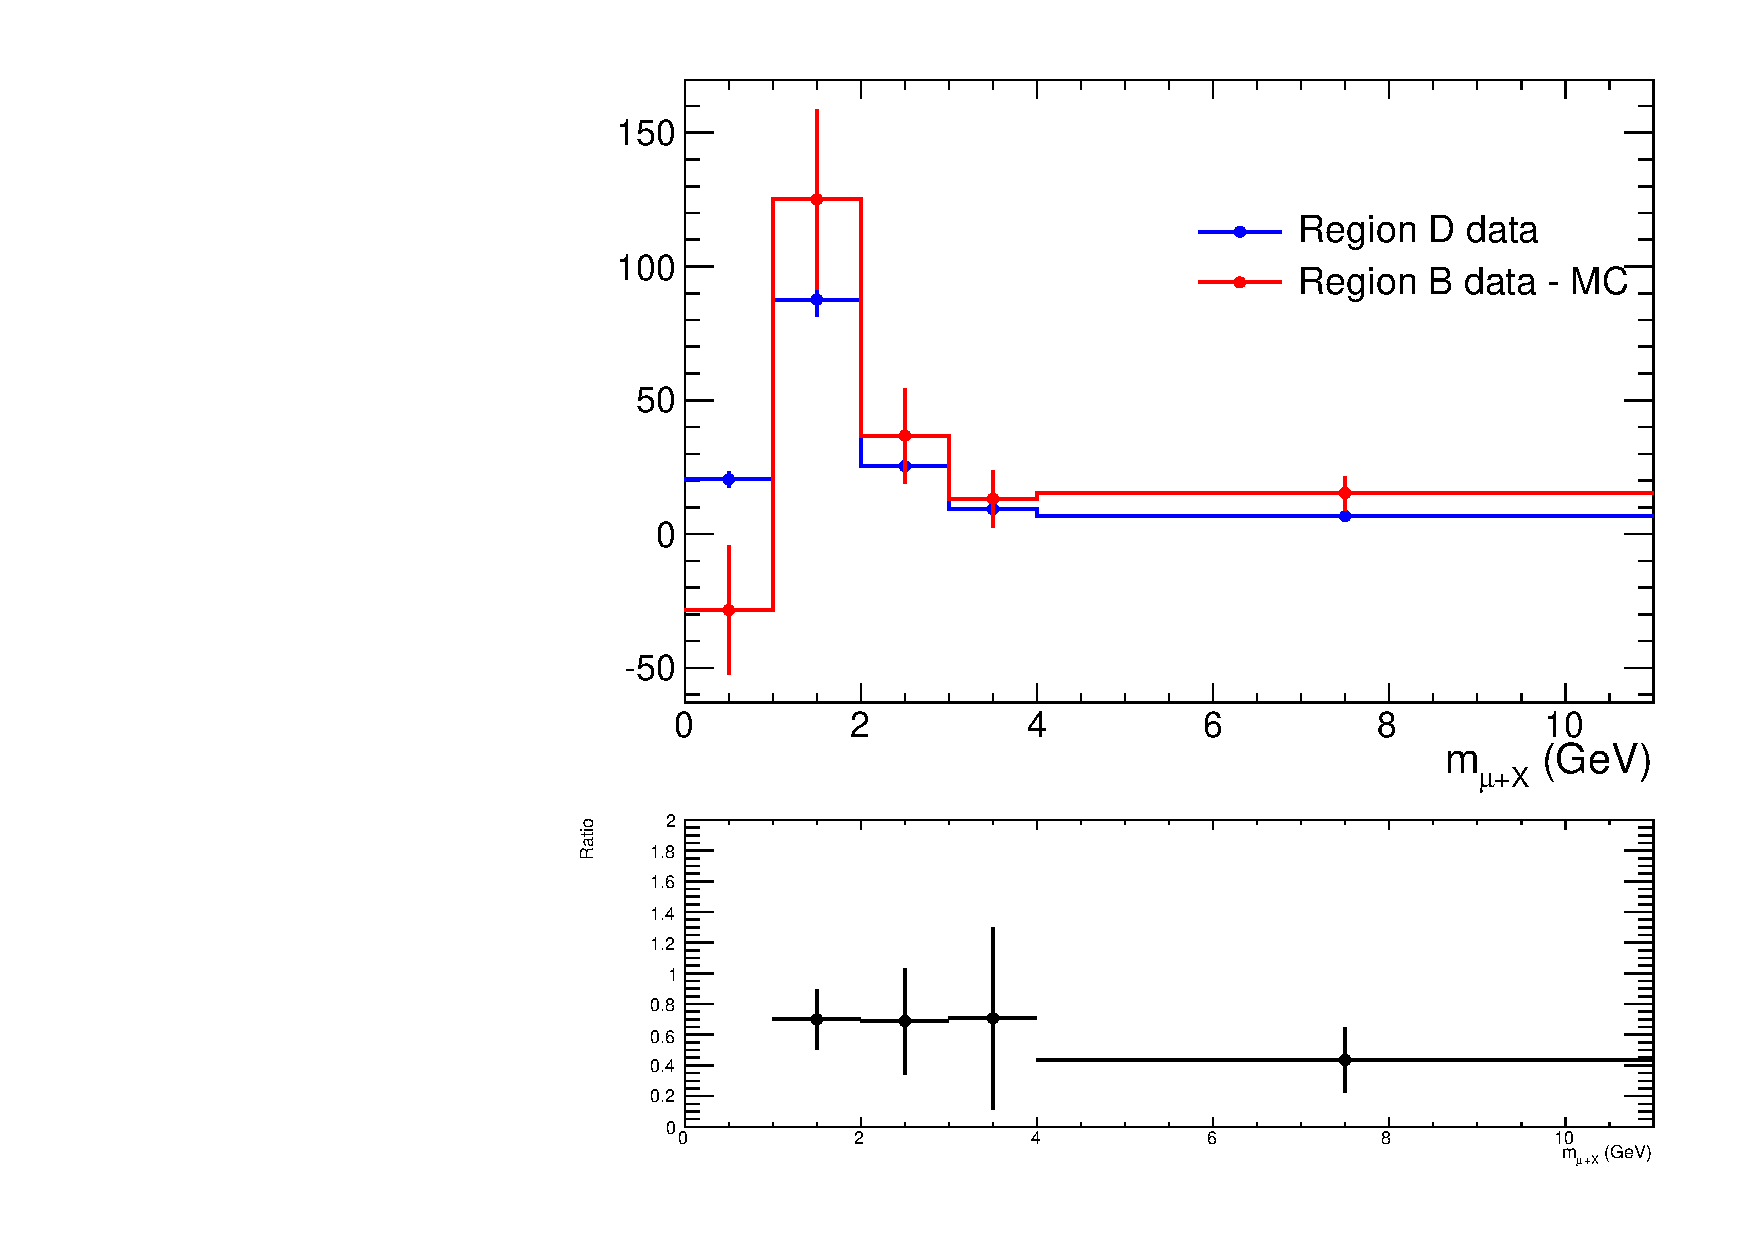
\includegraphics[width=\cmsFigWidth]{figures/muHadMassCanvas_regBDataMinusMCVsRegDData_lowMT}
    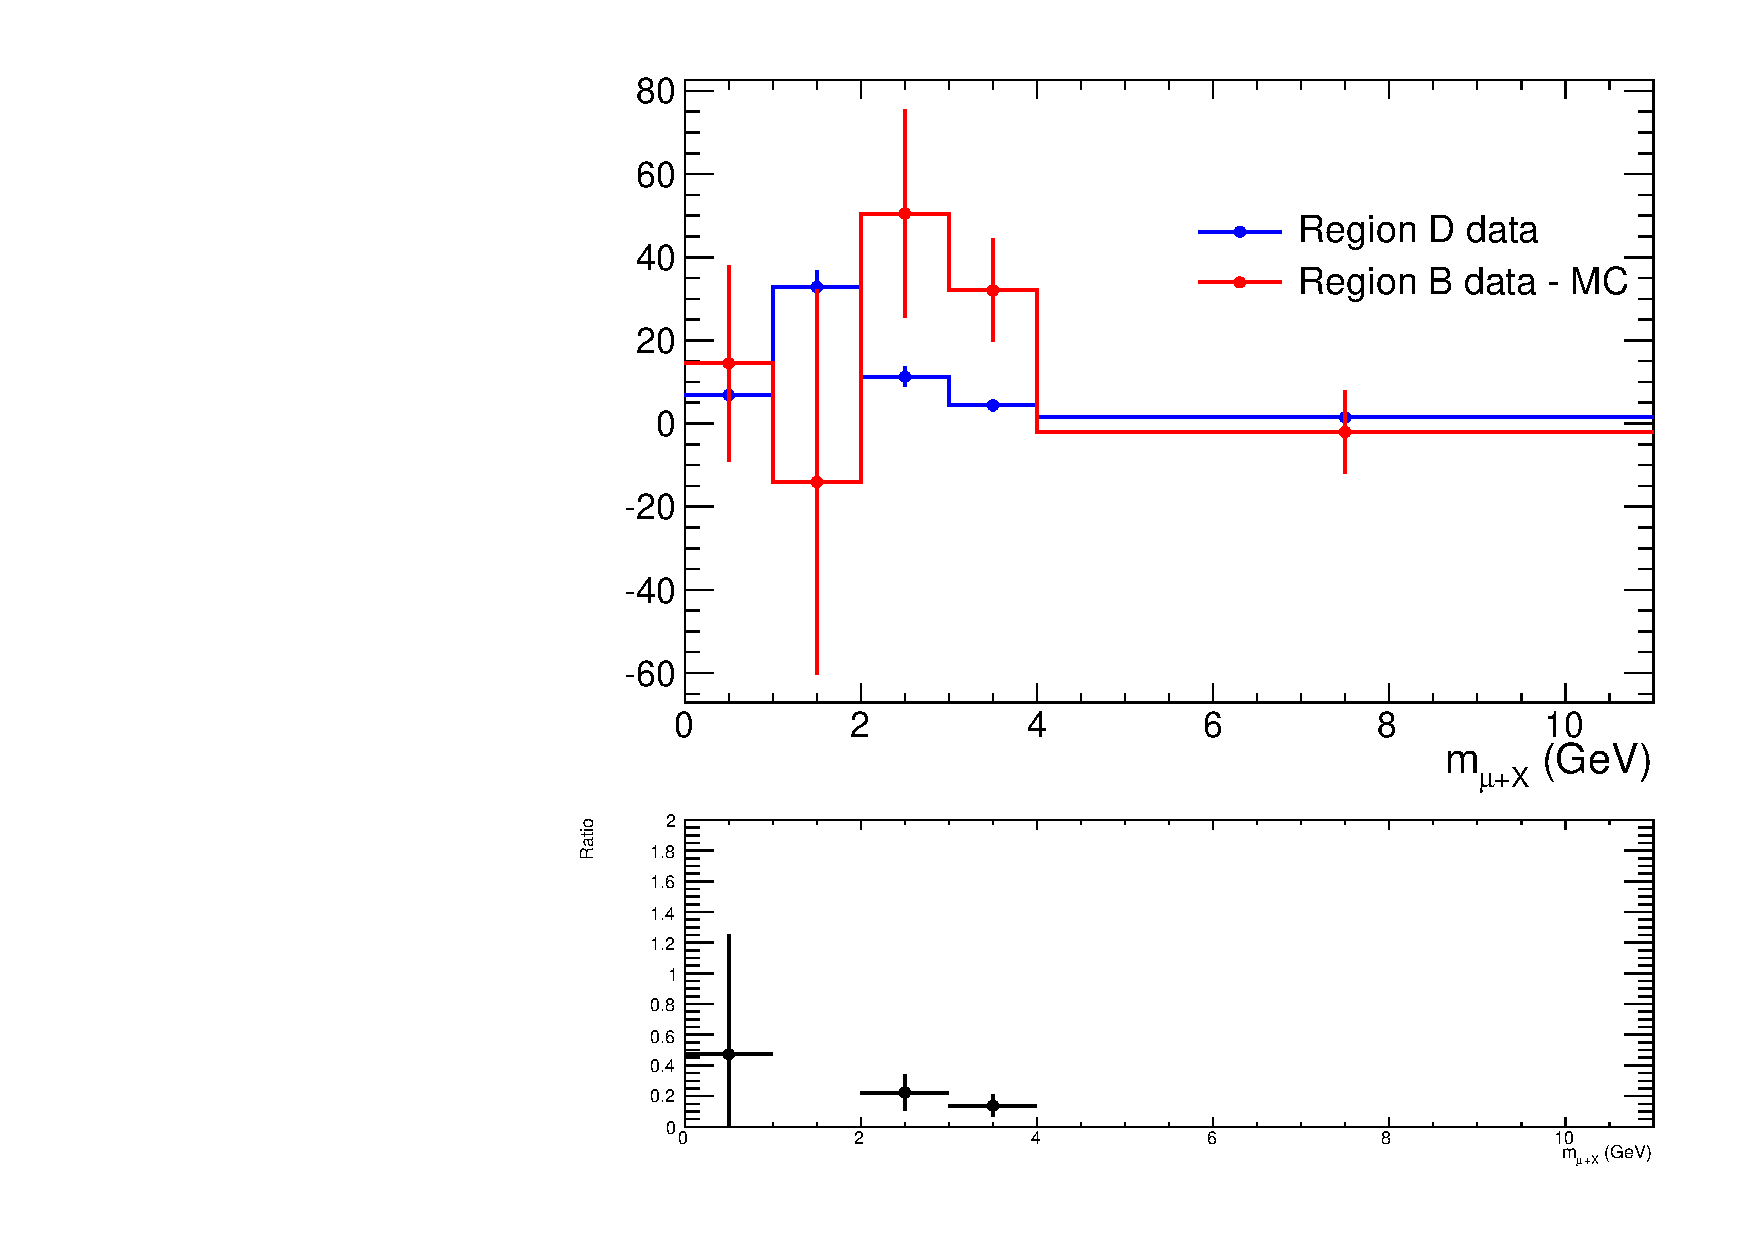
\includegraphics[width=\cmsFigWidth]{figures/muHadMassCanvas_regBDataMinusMCVsRegDData_highMT}
    \caption{Comparison of $m_{\mu+{\text{had}}}$ shapes between region D data and region B data minus total non-QCD backgrounds from simulation.  The region D distribution is normalized such that $N_{\text{D}}(m_{\mu+\text{had}} < 3\text{ }GeV)$ = $N_{\text{B}}^{\text{data - MC}}(m_{\mu+\text{had}} < 3\text{ }GeV)$.  (\cmsLeft) Low $M_{\text{T}}$. (\cmsRight) High $M_{\text{T}}$.}
    \label{fig:QCDComparisonBD}
  \end{center}
\end{figure}

Table~\ref{tab:regB-predictions} shows the breakdown of the expected SM contributions and observed data above $m_{\mu+\text{had}}$ = 4 GeV in the isolation sideband control region B, including statistical errors.  Figures~\ref{fig:regB-data-MC-nGoodVtx}-\ref{fig:regB-data-MC-tauMuPT} show some comparisons between region B data, region B MC, and the region B QCD prediction (which is taken from region D).

\begin{table*}[htbH]
\begin{center}
\caption{Expected SM events (from MC; QCD from region D data) and observed events above $m_{\mu+\text{had}}$ = 4 GeV in Region B.  The MC backgrounds are normalized to 19.7 fb$^{-1}$.  The QCD normalization is given by Eqs.~\ref{eq:f-B-QCD} and~\ref{eq:R-B-QCD}.\label{tab:regB-predictions}}
\begin{tabular}{lll}
\hline & $\text{M}_{\text{T}}$ $\le$ 50 GeV & $\text{M}_{\text{T}}$ $>$ 50 GeV \\
\hline
WW & 0 & 0 \\
ZZ & 0.0421 $\pm$ 0.042 & 0.235 $\pm$ 0.097 \\
WZ & 0 & 0.276 $\pm$ 0.14 \\
W + jets & 0.367 $\pm$ 0.37 & 6.29 $\pm$ 2.8 \\
Single top & 0.373 $\pm$ 0.32 & 0.69 $\pm$ 0.43 \\
$t\bar{t}$ & 0 & 14.6 $\pm$ 8.6 \\
Drell-Yan + jets & 5.92 $\pm$ 4.3 & 0 \\
QCD (from data) & 7.23 $\pm$ 2.8 & 2.09 $\pm$ 2 \\
\hline
Tot. expected SM & 13.9 $\pm$ 5.1 & 24.1 $\pm$ 9.2 \\
\hline
Data & 22 & 20 \\
\hline
\end{tabular}
\end{center}
\end{table*}

\begin{figure}[hbtp]
  \begin{center}
    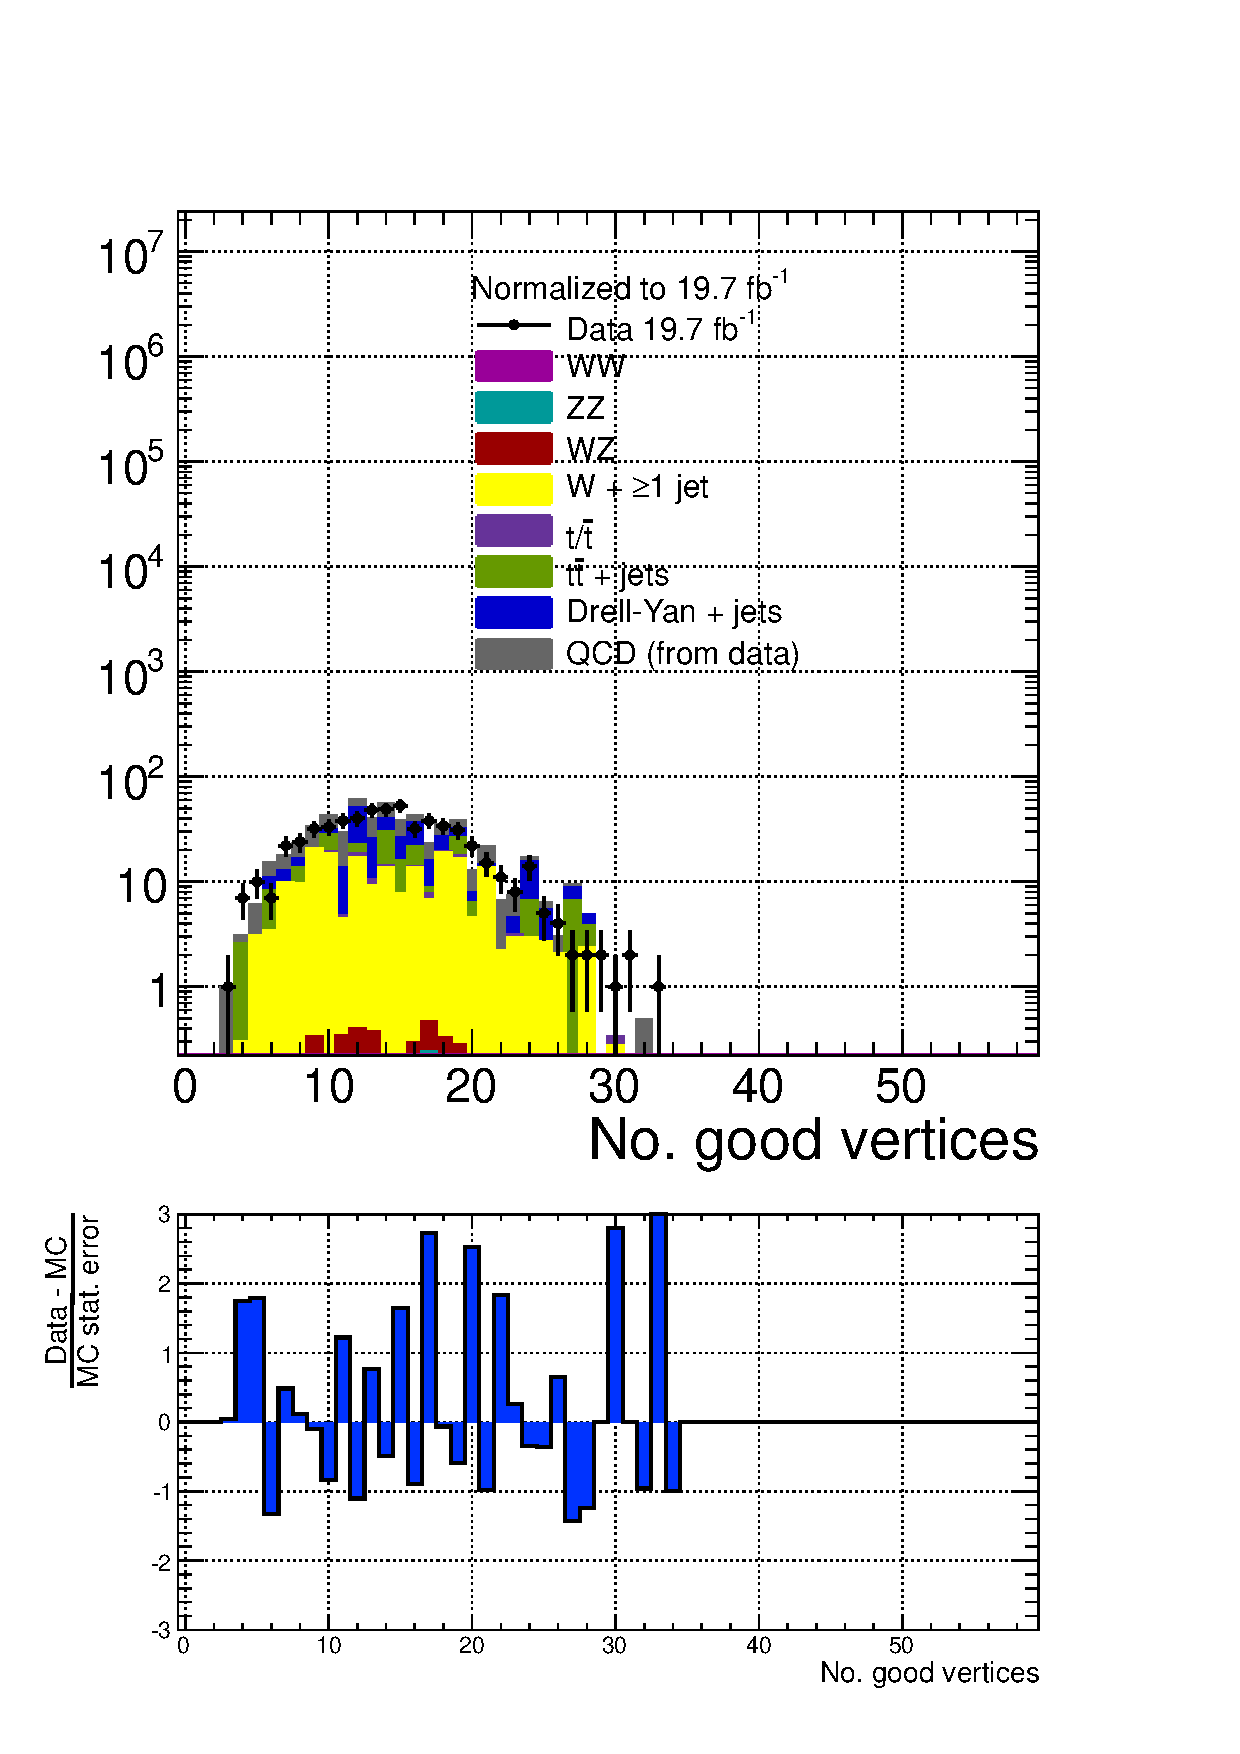
\includegraphics[width=\cmsFigWidth]{figures/dataVsMCQCD_nGoodVtx_lowMT_v87}
    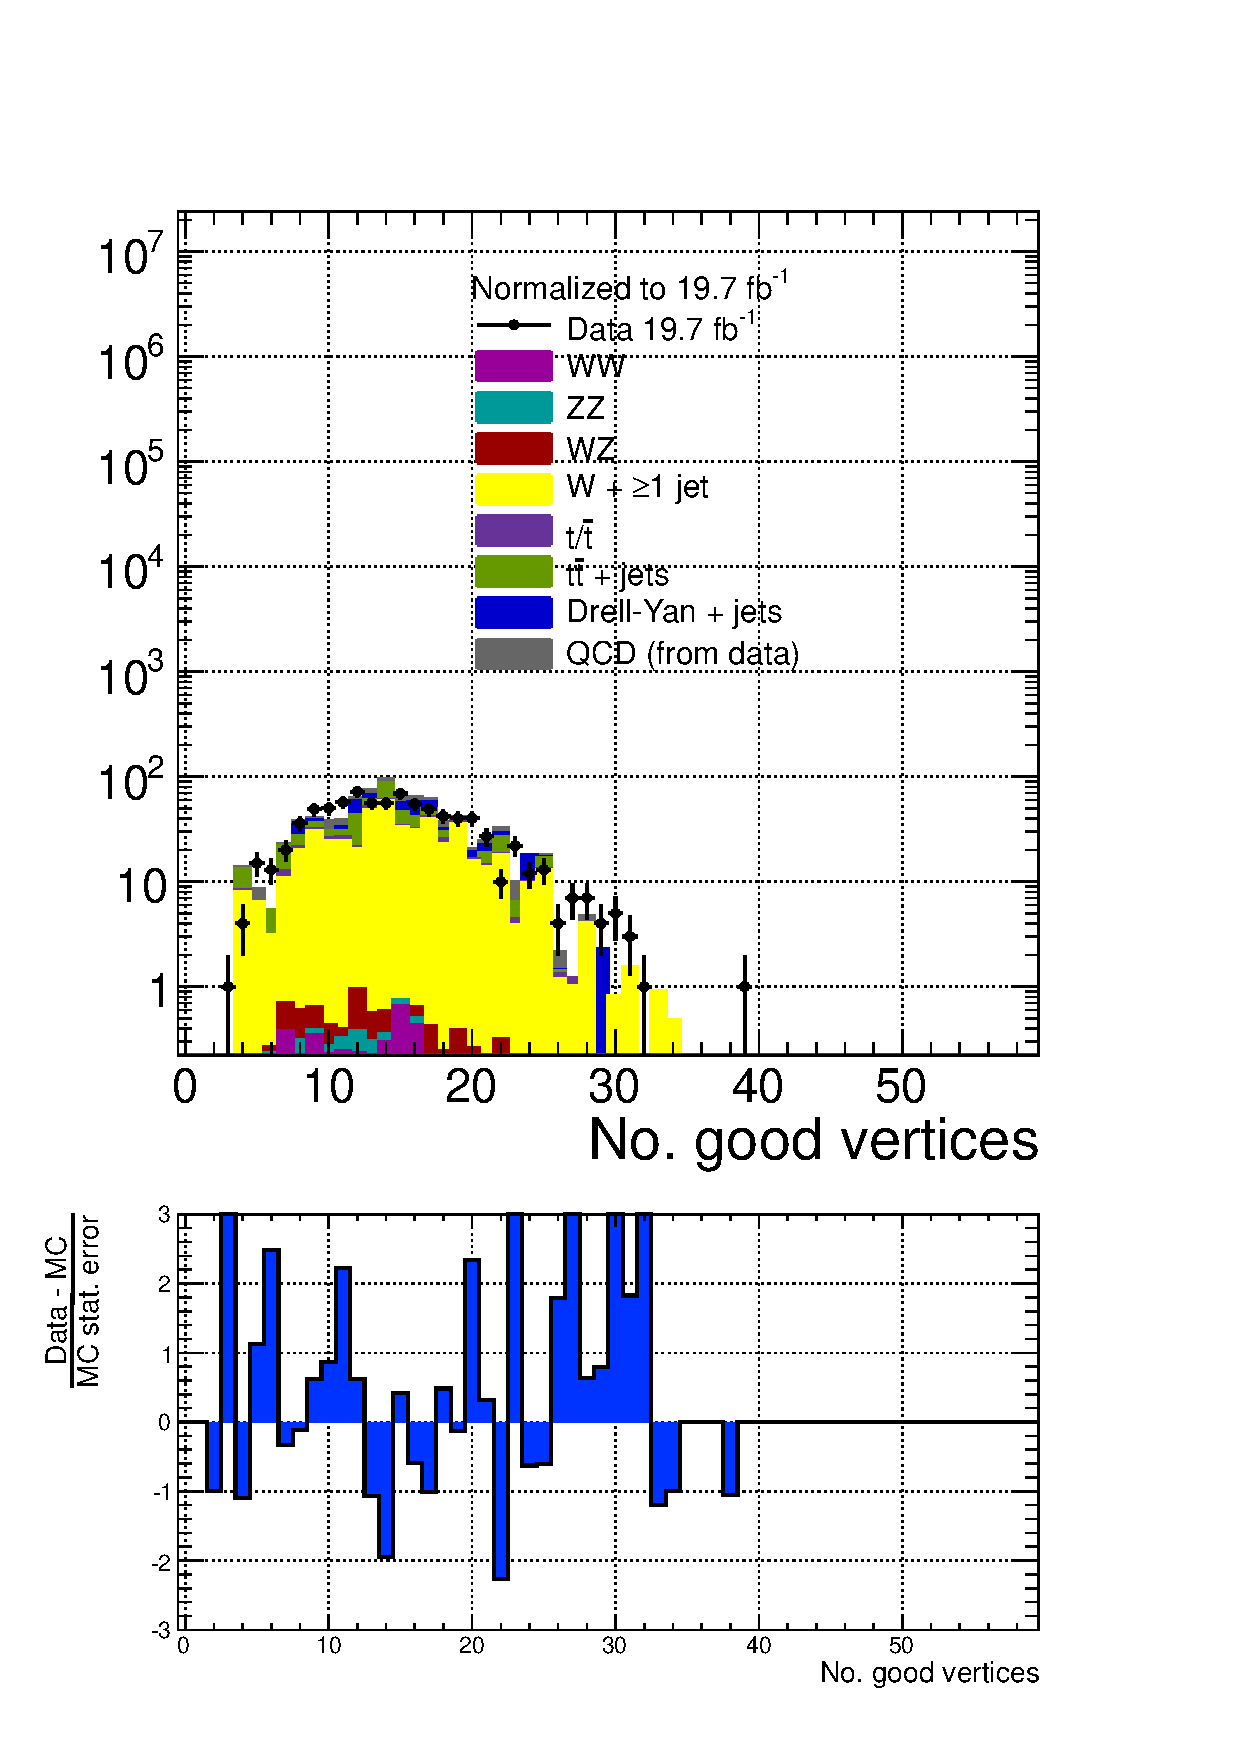
\includegraphics[width=\cmsFigWidth]{figures/dataVsMCQCD_nGoodVtx_highMT_v87}
    \caption{Distribution of the number of good reconstructed vertices for region B data (black points), region B total non-QCD backgrounds from MC (solid stacked histograms), and the QCD prediction from region D data (solid gray histogram).  A good reconstructed vertex is required to not be fake, have $>$4 degrees of freedom, have z position $\le$24 \cm, and have radial position $\le$2 \cm.  Errors are statistical only. (\cmsLeft) Low-$M_{\text{T}}$ bin. (\cmsRight) High-$M_{\text{T}}$ bin.}
    \label{fig:regB-data-MC-nGoodVtx}
  \end{center}
\end{figure}

\begin{figure}[hbtp]
  \begin{center}
    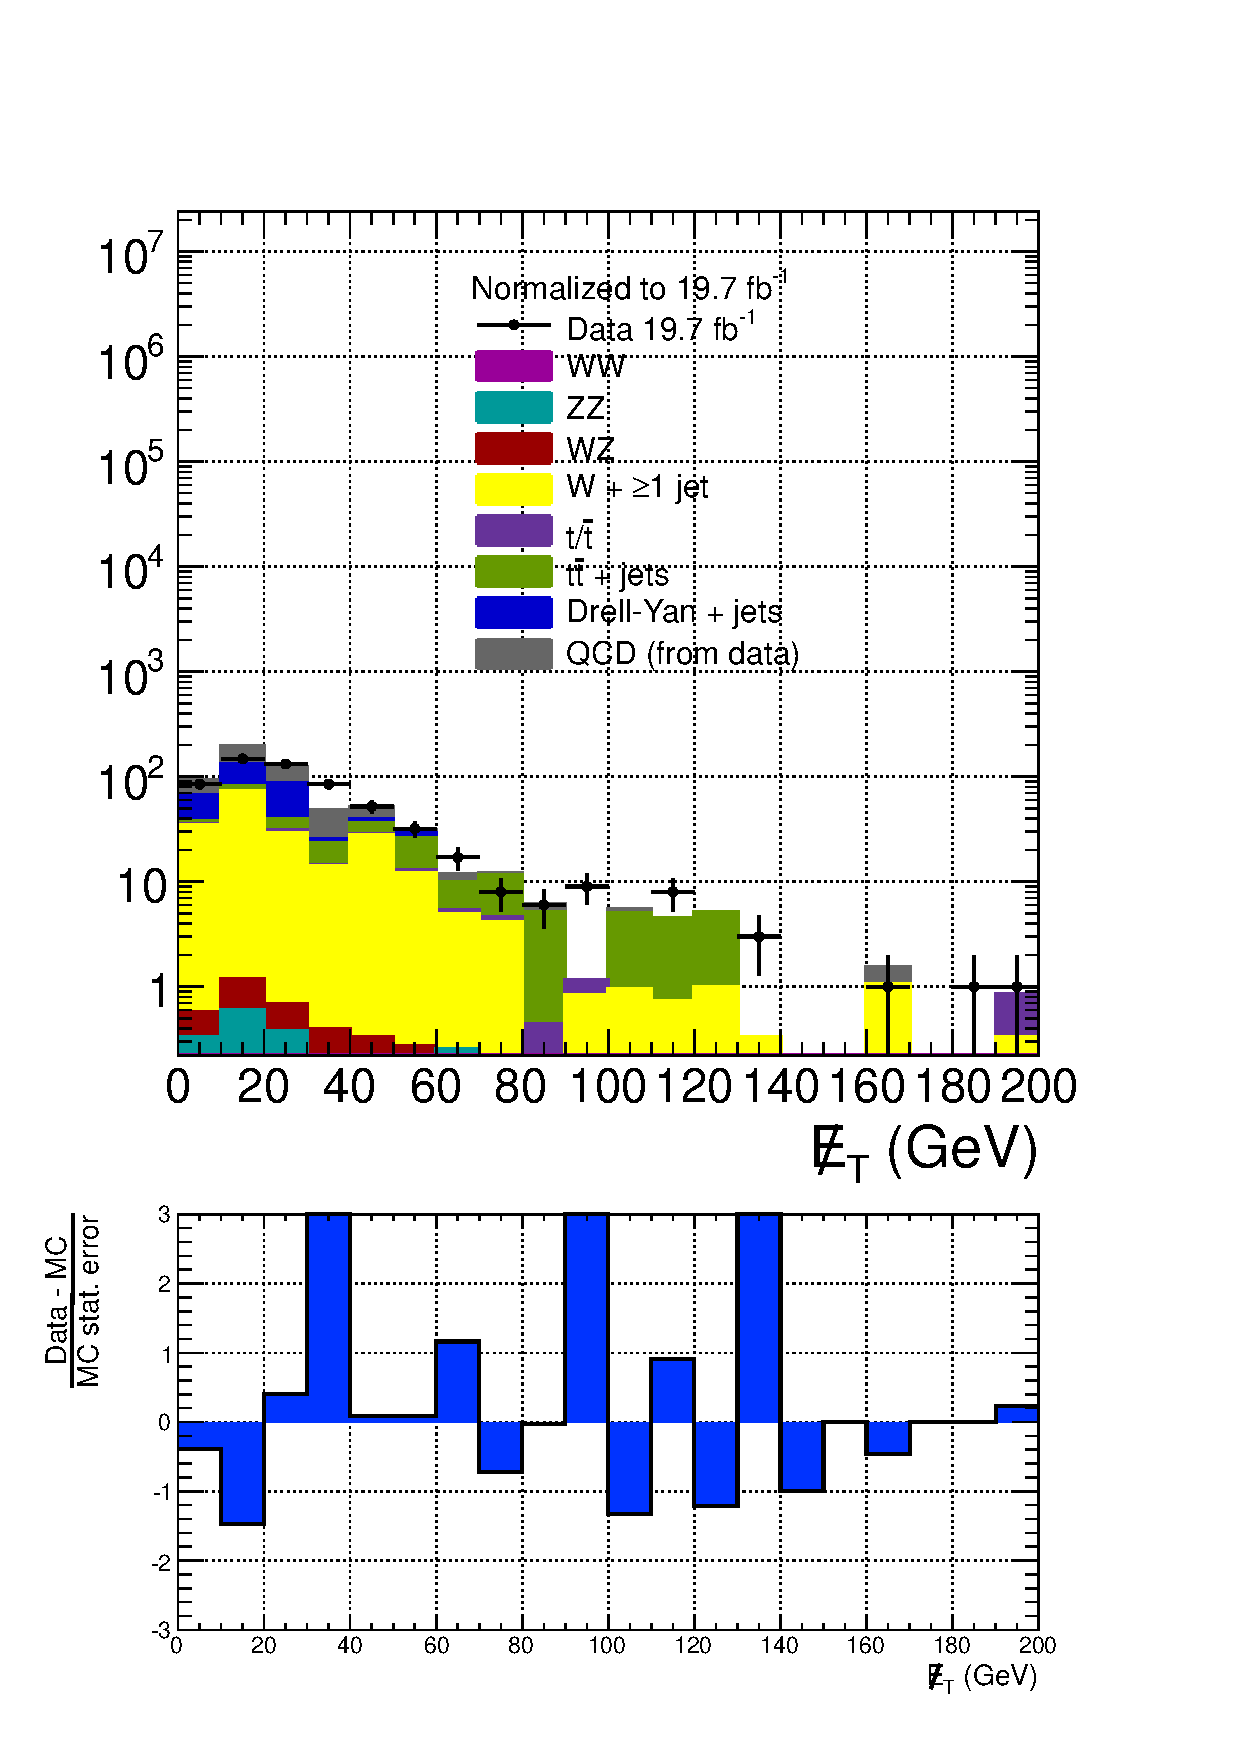
\includegraphics[width=\cmsFigWidth]{figures/dataVsMCQCD_MET_lowMT_v87}
    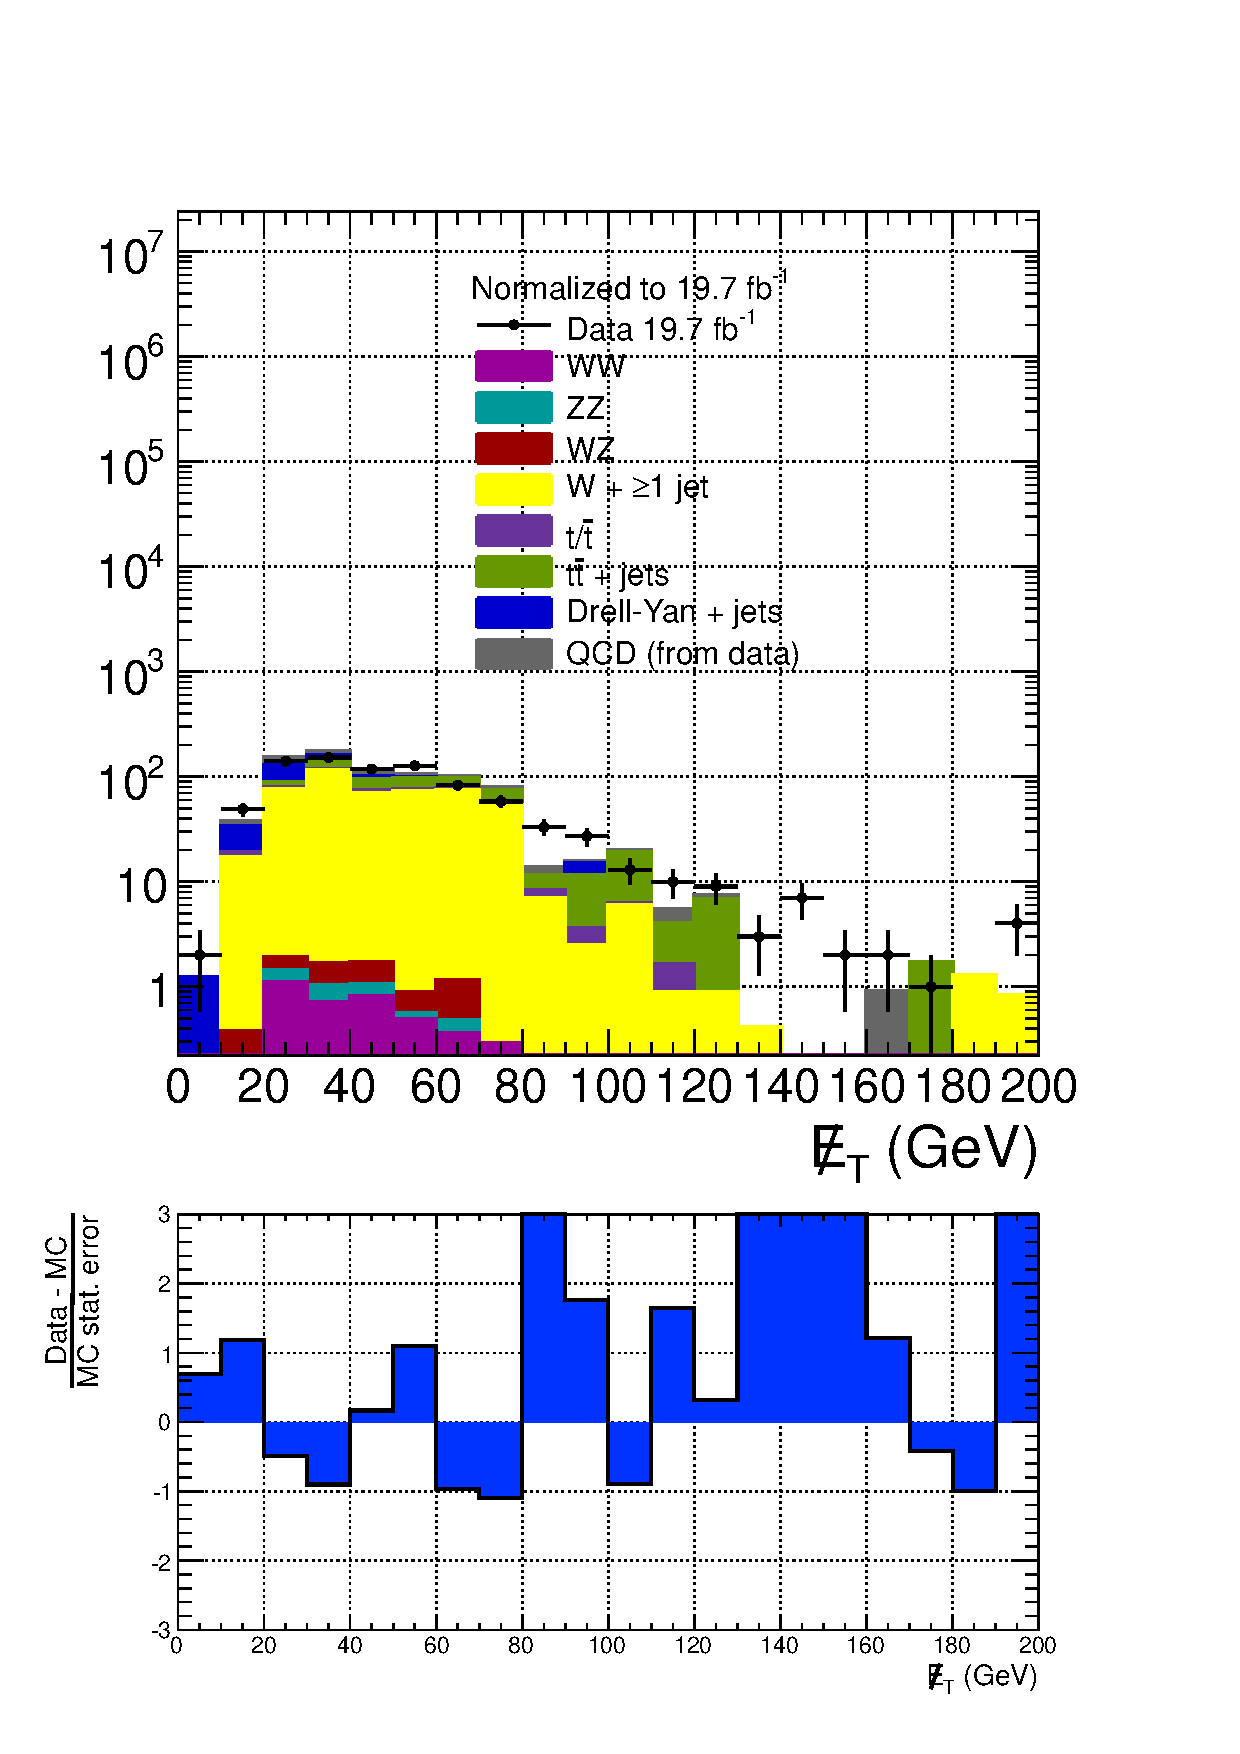
\includegraphics[width=\cmsFigWidth]{figures/dataVsMCQCD_MET_highMT_v87}
    \caption{\ETslash distribution for region B data (black points), region B total non-QCD backgrounds from MC (solid stacked histograms), and the QCD prediction from region D data (solid gray histogram).  Errors are statistical only. (\cmsLeft) Low-$M_{\text{T}}$ bin. (\cmsRight) High-$M_{\text{T}}$ bin.}
    \label{fig:regB-data-MC-MET}
  \end{center}
\end{figure}

\begin{figure}[hbtp]
  \begin{center}
    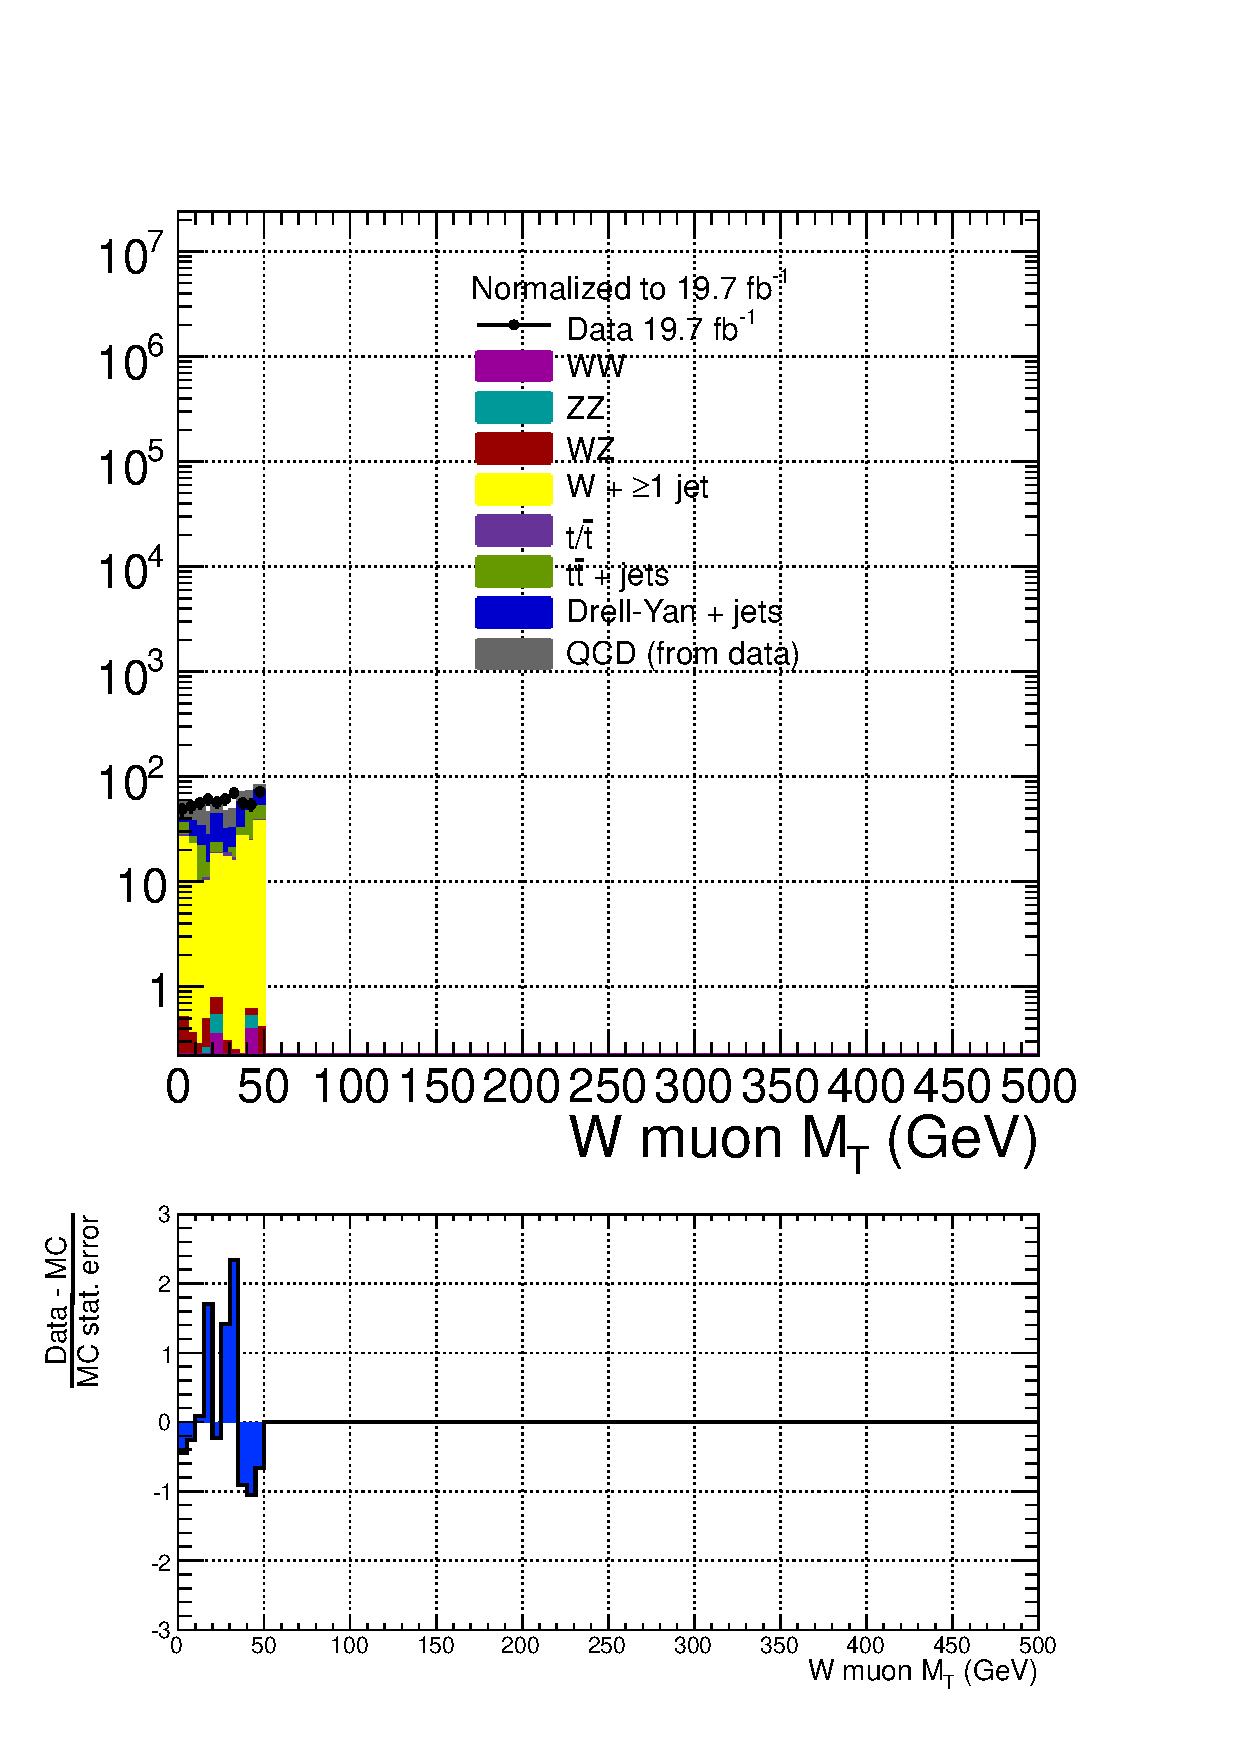
\includegraphics[width=\cmsFigWidth]{figures/dataVsMCQCD_WMuMT_lowMT_v87}
    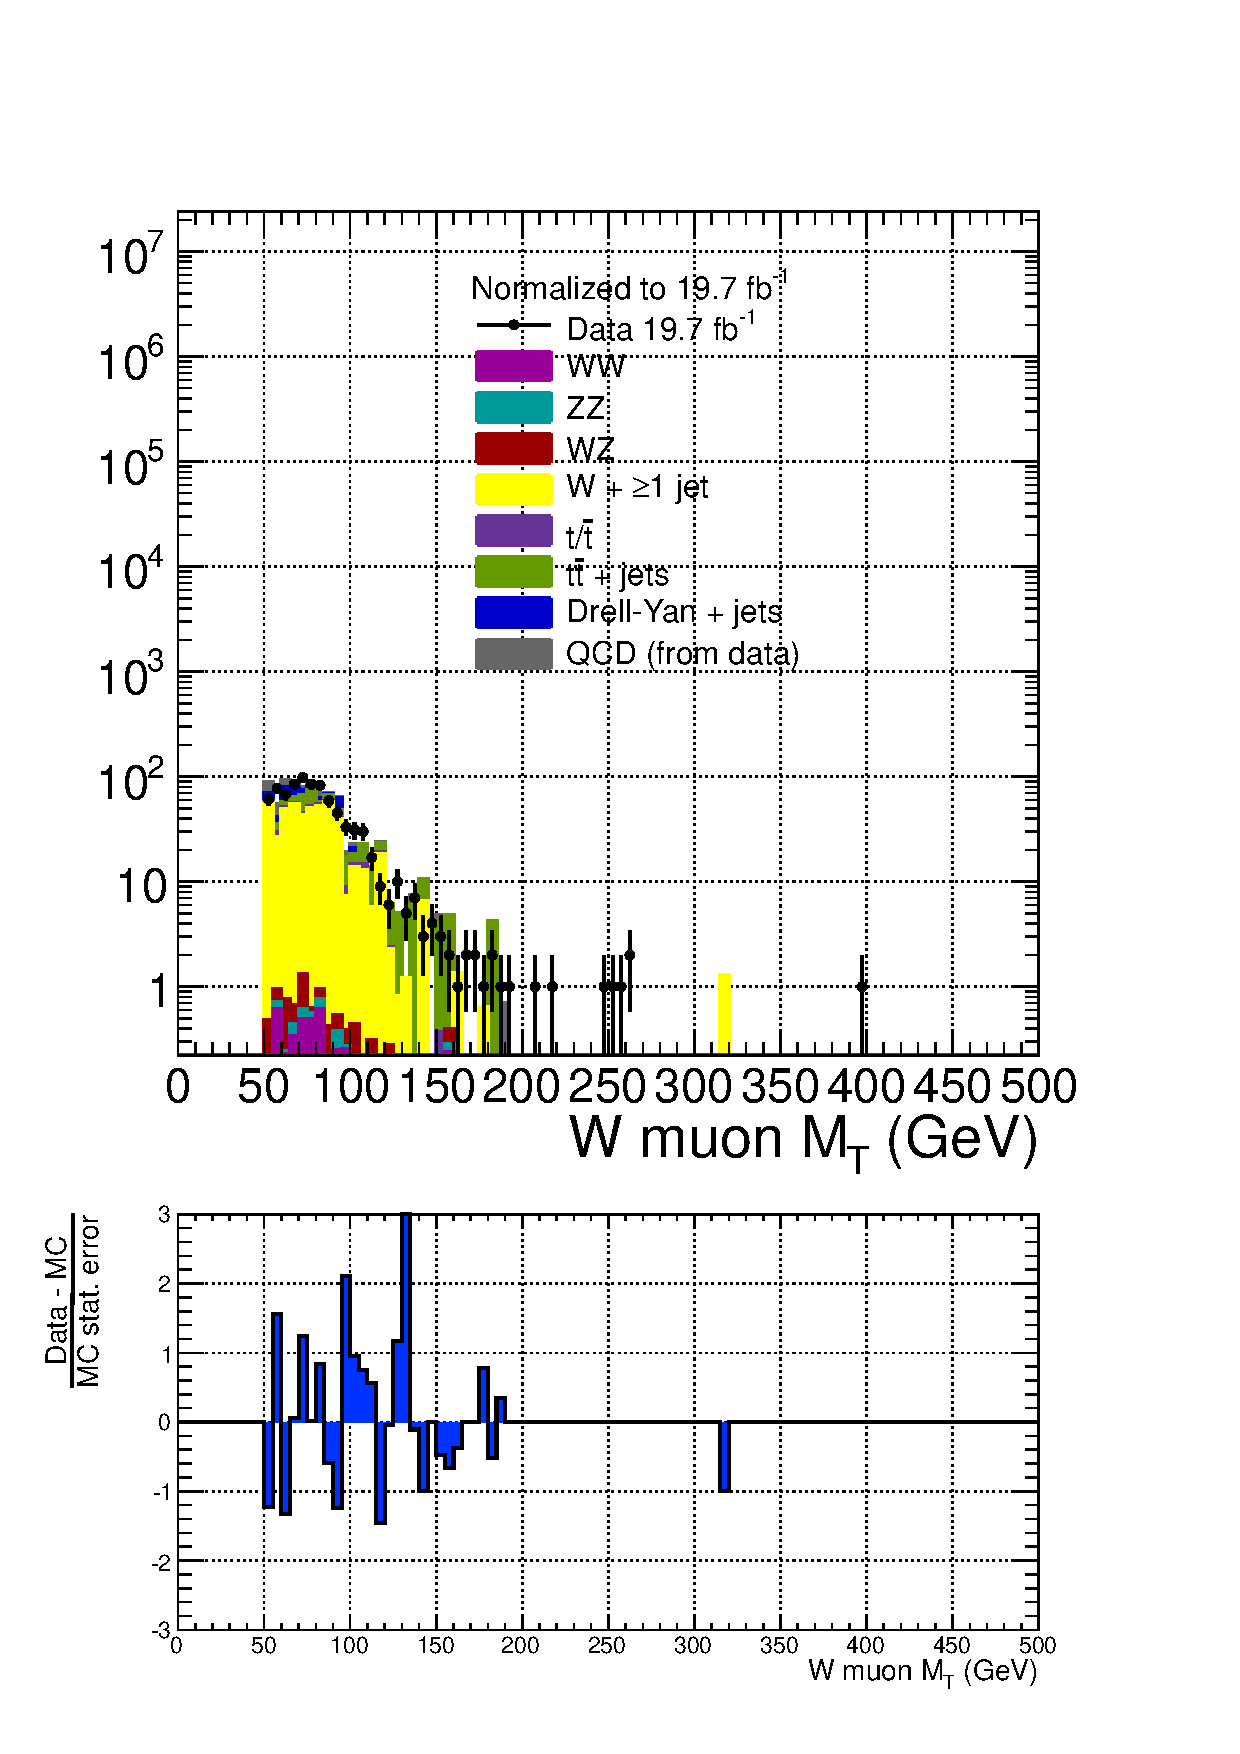
\includegraphics[width=\cmsFigWidth]{figures/dataVsMCQCD_WMuMT_highMT_v87}
    \caption{Trigger muon $M_{\text{T}}$ distribution for region B data (black points), region B total non-QCD backgrounds from MC (solid stacked histograms), and the QCD prediction from region D data (solid gray histogram).  Errors are statistical only. The term ``$W$ muon'' in the label refers to the trigger muon, not necessarily a muon from a $W$ decay (as in the case of the $ggH$ signal, for instance).  (\cmsLeft) Low-$M_{\text{T}}$ bin. (\cmsRight) High-$M_{\text{T}}$ bin.}
    \label{fig:regB-data-MC-MT}
  \end{center}
\end{figure}

\begin{figure}[hbtp]
  \begin{center}
    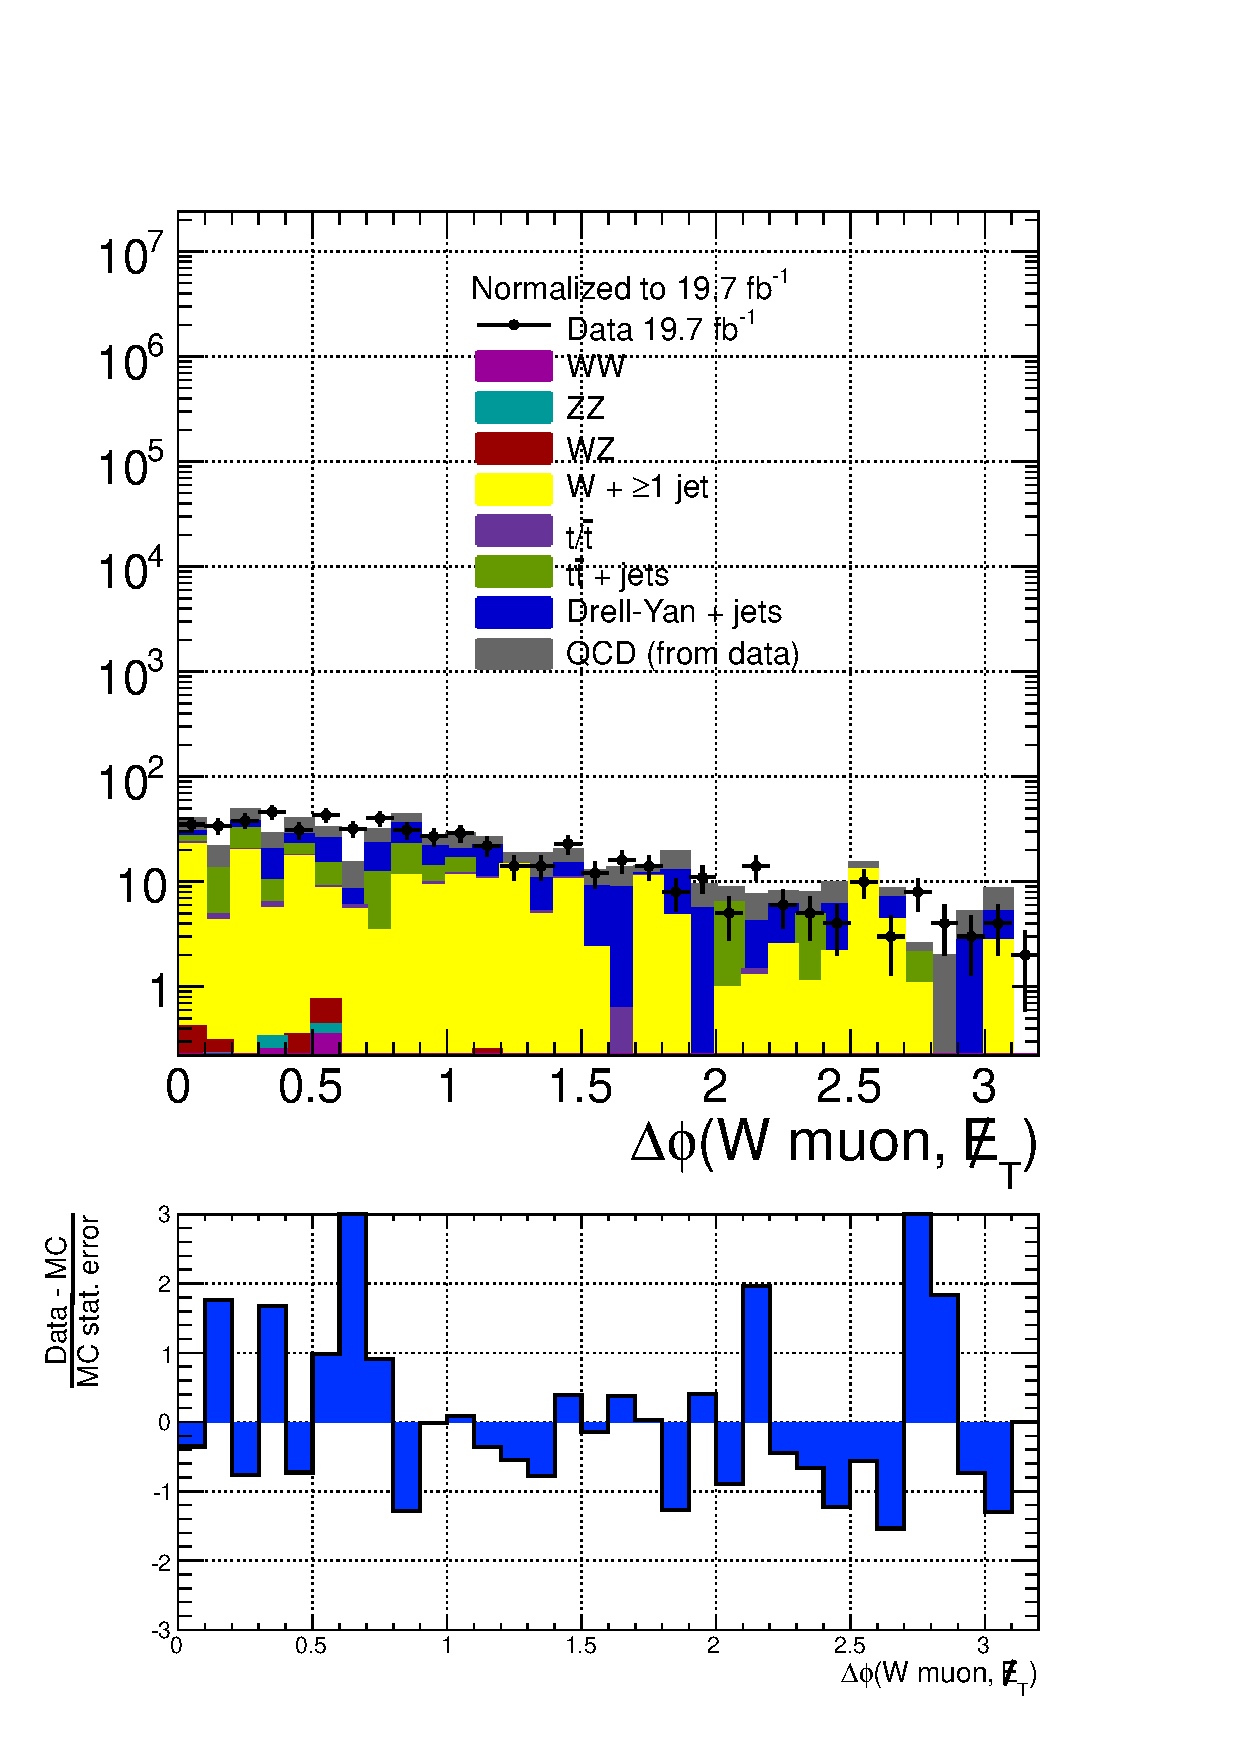
\includegraphics[width=\cmsFigWidth]{figures/dataVsMCQCD_dPhiWMuMET_lowMT_v87}
    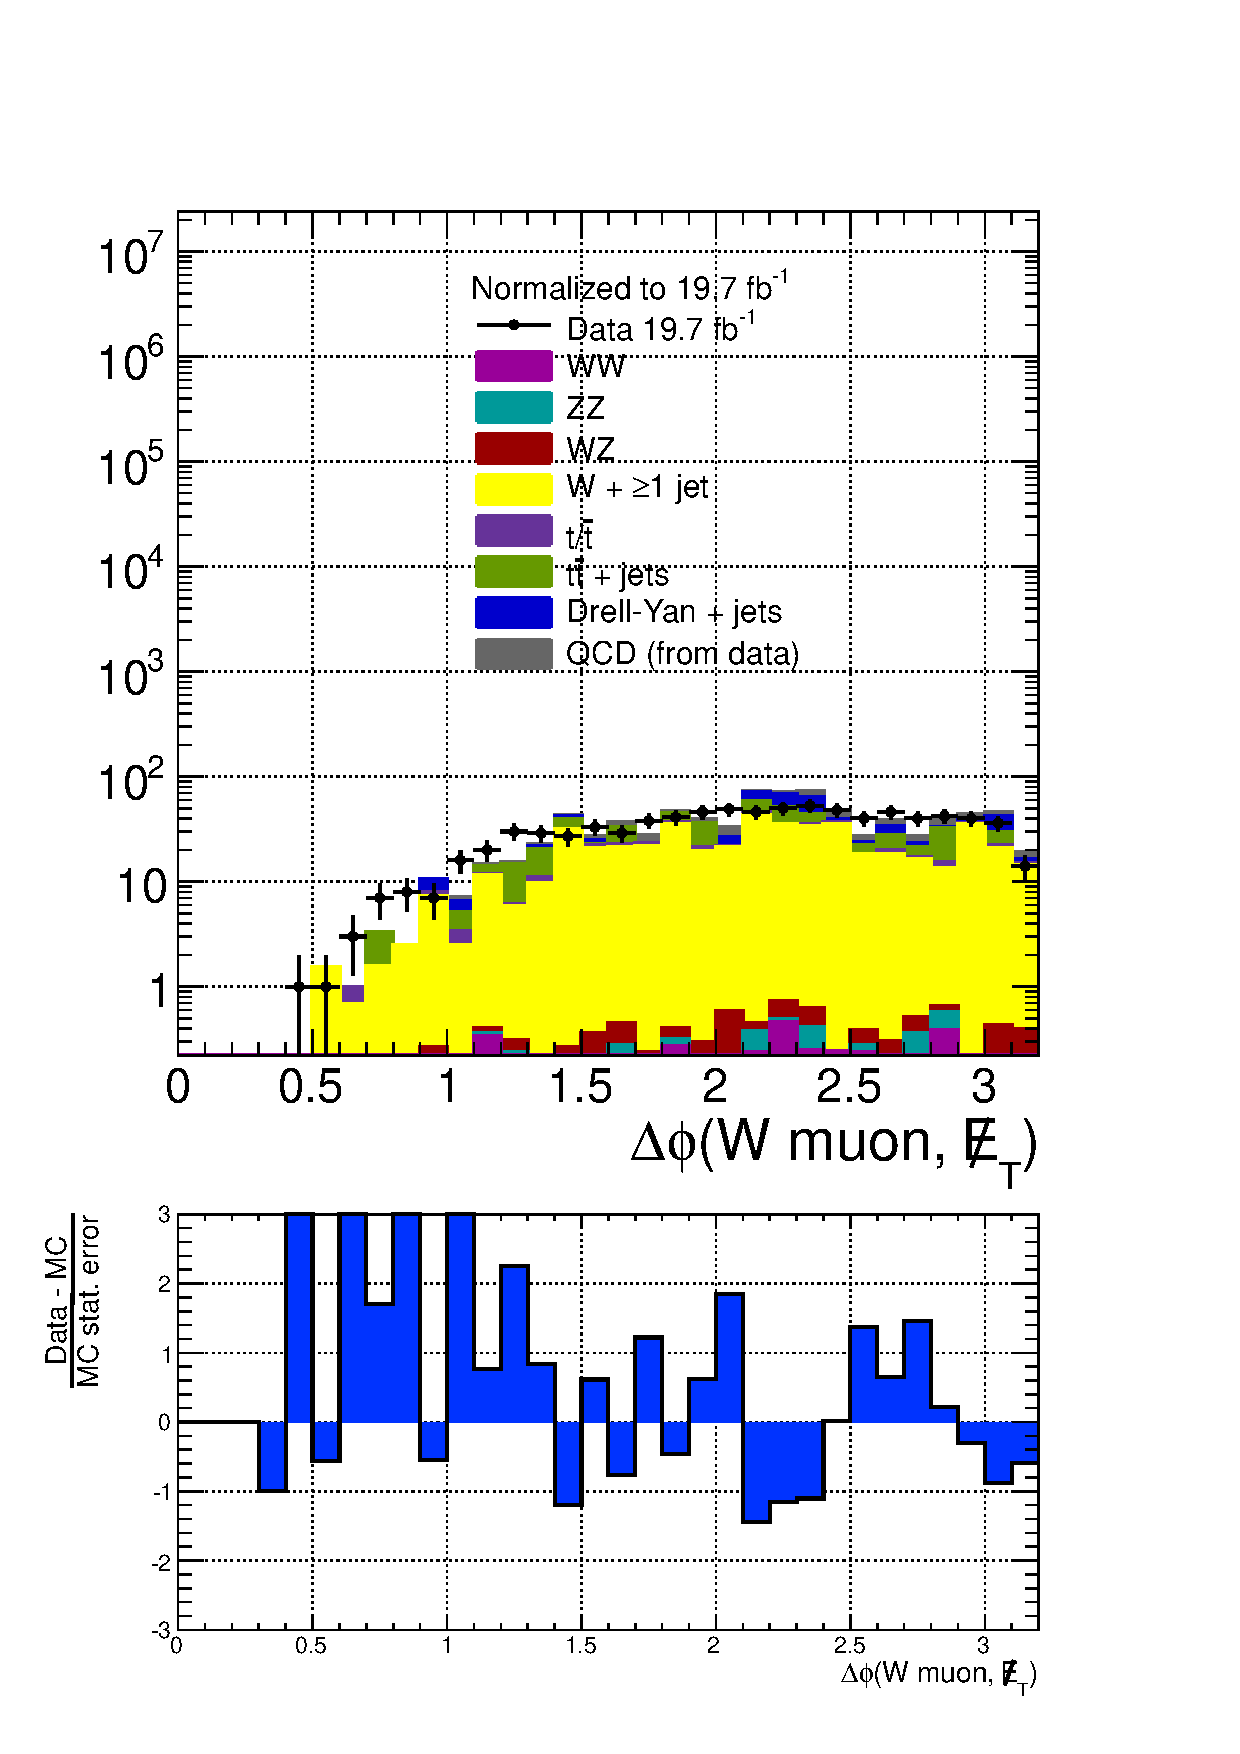
\includegraphics[width=\cmsFigWidth]{figures/dataVsMCQCD_dPhiWMuMET_highMT_v87}
    \caption{$\Delta\phi$(trigger muon, \ETslash) distribution for region B data (black points), region B total non-QCD backgrounds from MC (solid stacked histograms), and the QCD prediction from region D data (solid gray histogram).  Errors are statistical only. The term ``$W$ muon'' in the label refers to the trigger muon, not necessarily a muon from a $W$ decay (as in the case of the $ggH$ signal, for instance).  (\cmsLeft) Low-$M_{\text{T}}$ bin. (\cmsRight) High-$M_{\text{T}}$ bin.}
    \label{fig:regB-data-MC-dPhiWMuMET}
  \end{center}
\end{figure}

\begin{figure}[hbtp]
  \begin{center}
    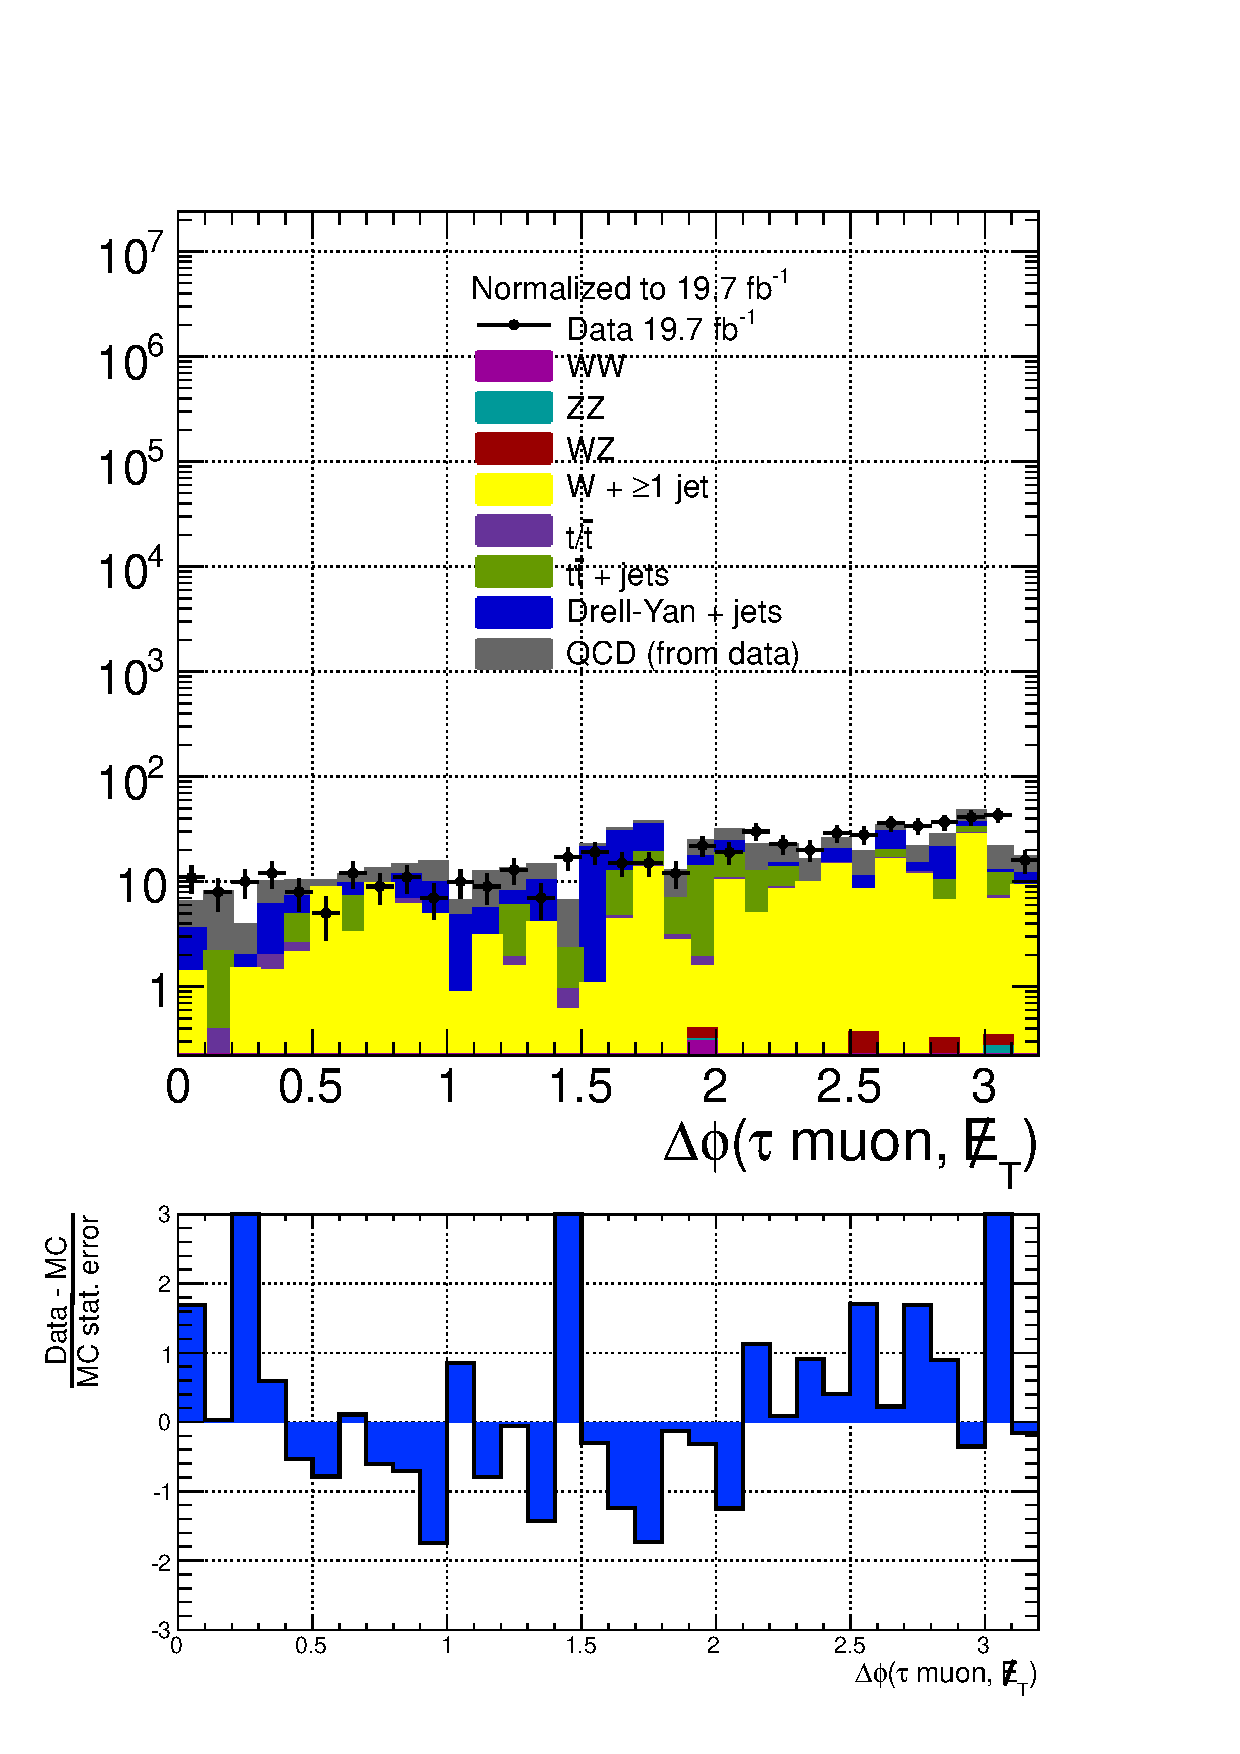
\includegraphics[width=\cmsFigWidth]{figures/dataVsMCQCD_dPhiTauMuMET_lowMT_v87}
    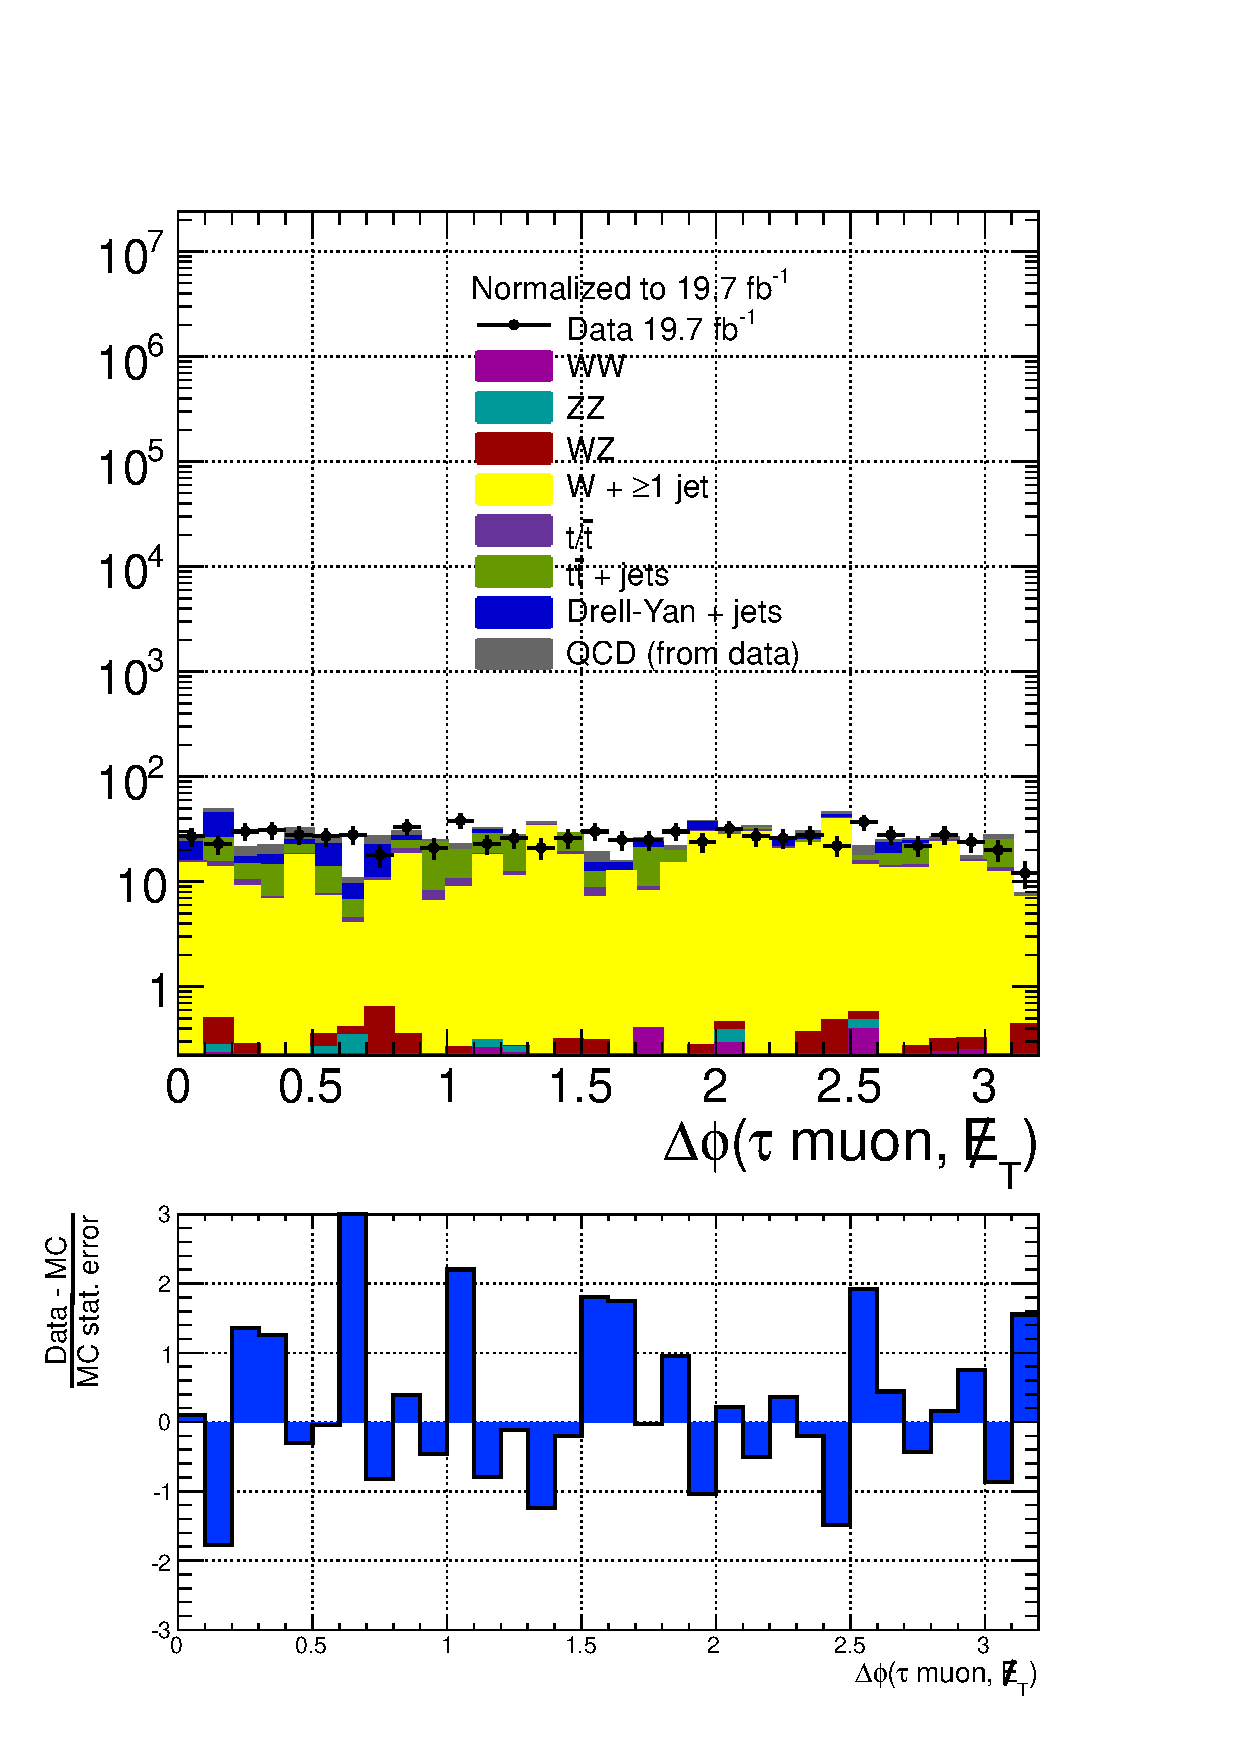
\includegraphics[width=\cmsFigWidth]{figures/dataVsMCQCD_dPhiTauMuMET_highMT_v87}
    \caption{$\Delta\phi$($\tau$ muon, \ETslash) distribution for region B data (black points), region B total non-QCD backgrounds from MC (solid stacked histograms), and the QCD prediction from region D data (solid gray histogram).  Errors are statistical only. (\cmsLeft) Low-$M_{\text{T}}$ bin. (\cmsRight) High-$M_{\text{T}}$ bin.}
    \label{fig:regB-data-MC-dPhiTauMuMET}
  \end{center}
\end{figure}

\begin{figure}[hbtp]
  \begin{center}
    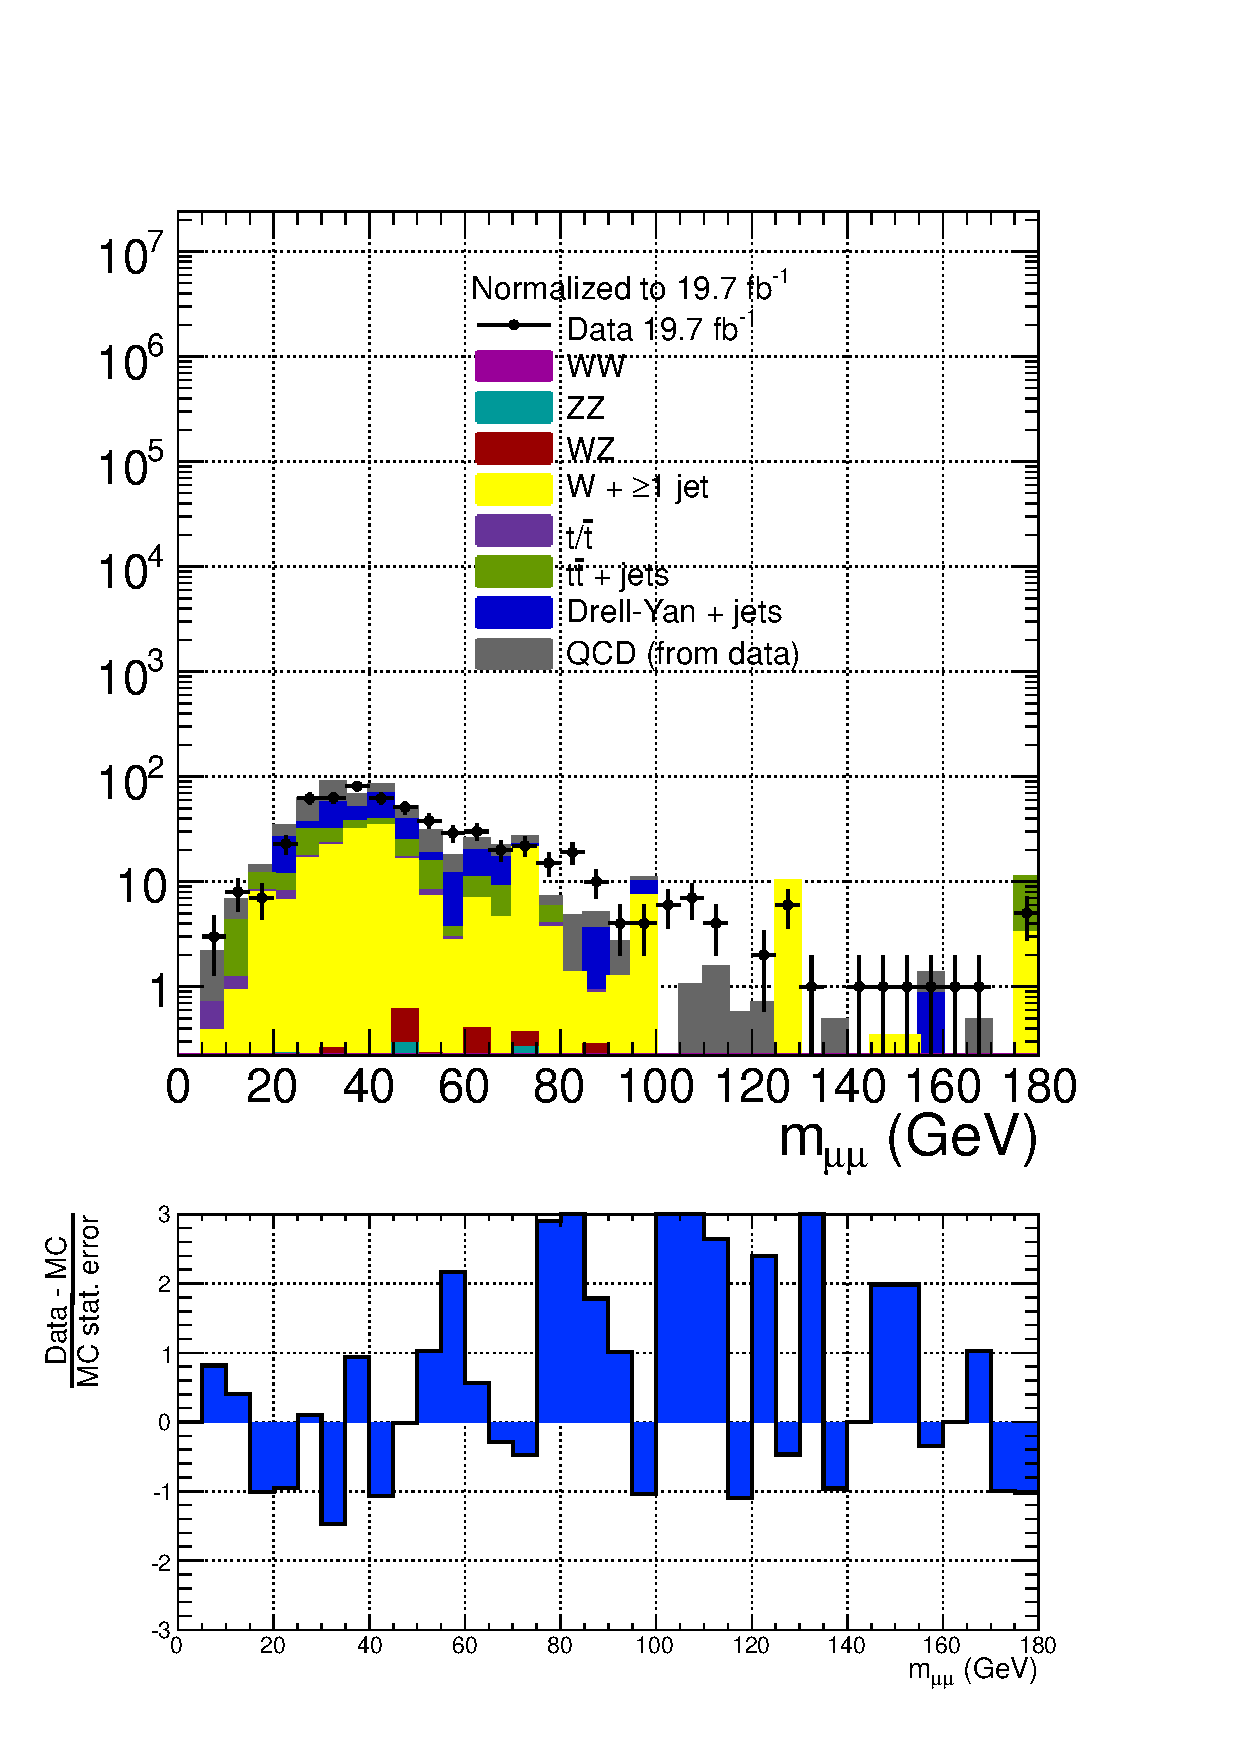
\includegraphics[width=\cmsFigWidth]{figures/dataVsMCQCD_mWMuTauMu_lowMT_v87}
    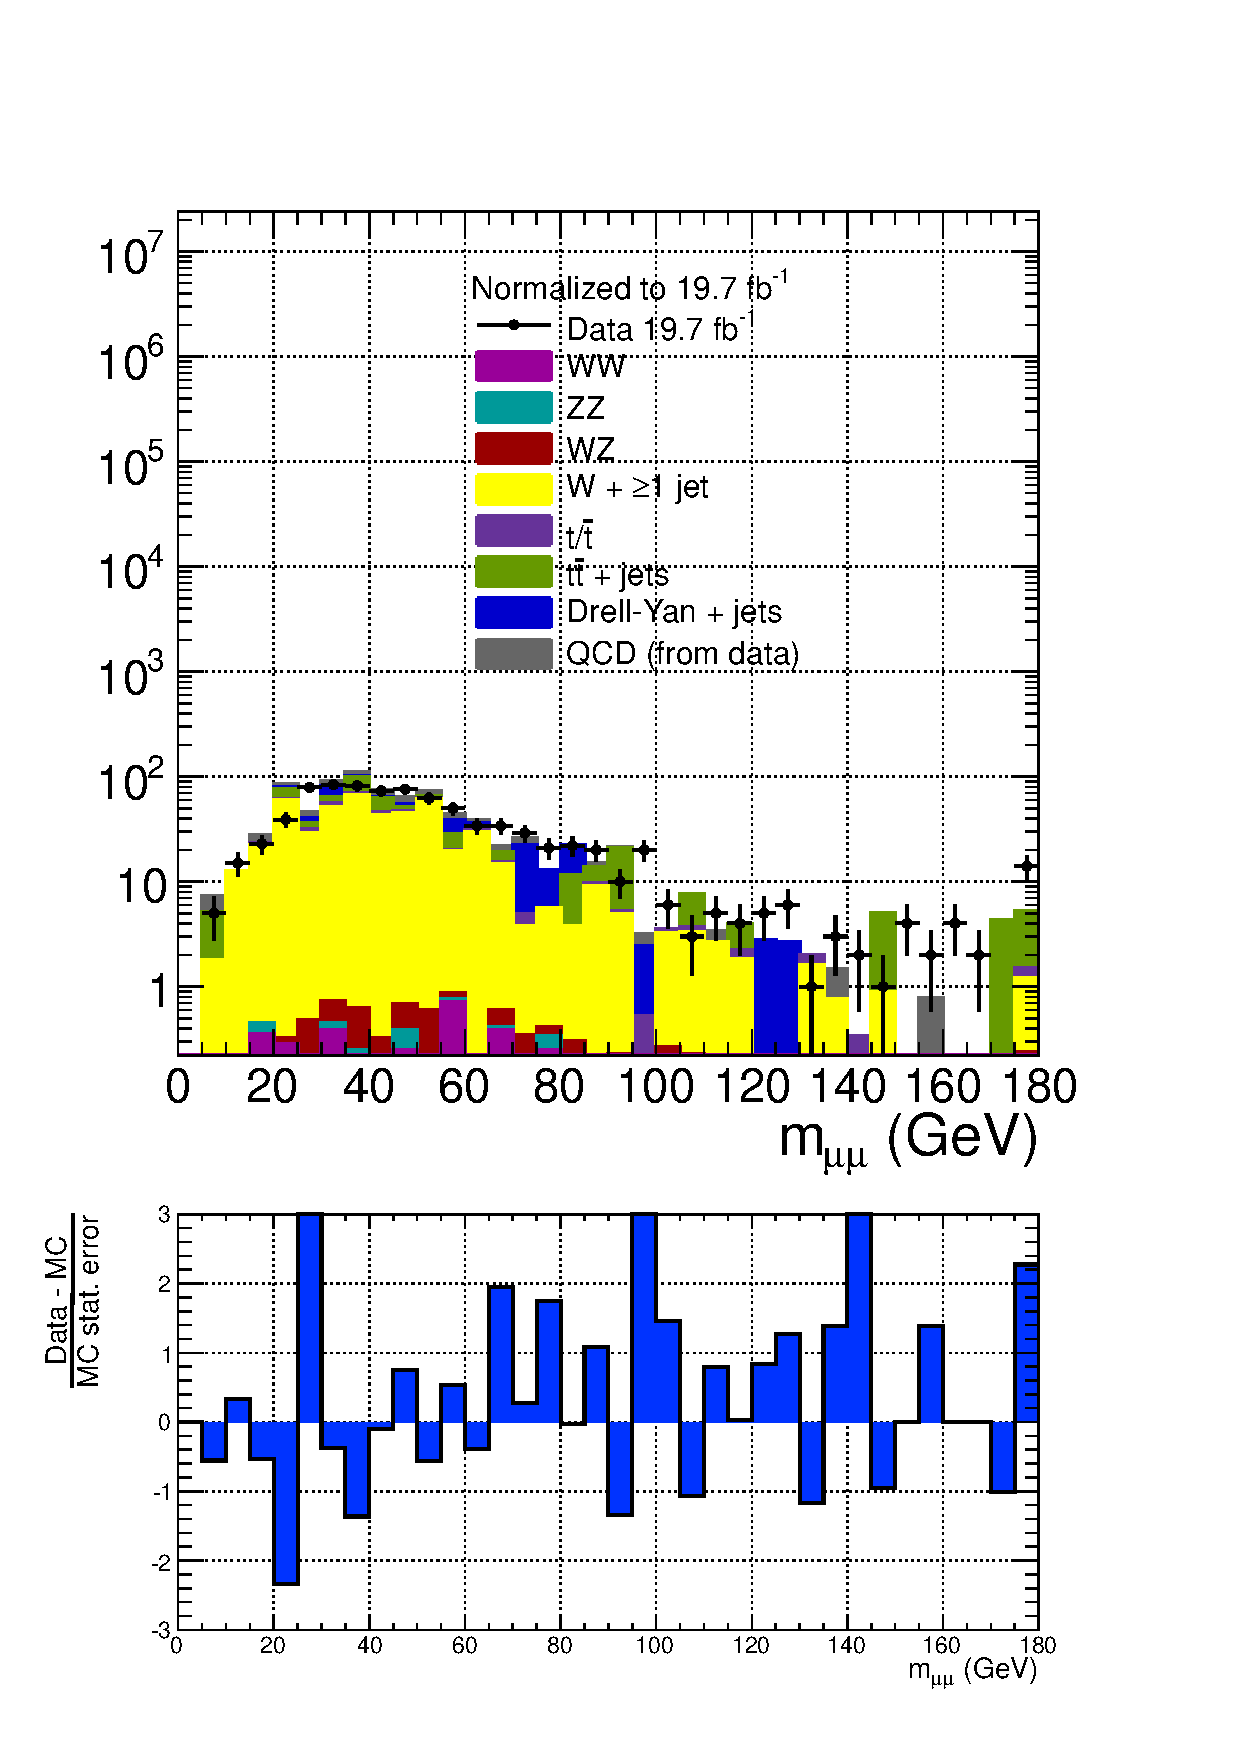
\includegraphics[width=\cmsFigWidth]{figures/dataVsMCQCD_mWMuTauMu_highMT_v87}
    \caption{Distribution of the invariant mass of the trigger muon and $\tau$ muon for region B data (black points), region B total non-QCD backgrounds from MC (solid stacked histograms), and the QCD prediction from region D data (solid gray histogram).  Errors are statistical only. (\cmsLeft) Low-$M_{\text{T}}$ bin. (\cmsRight) High-$M_{\text{T}}$ bin.}
    \label{fig:regB-data-MC-mWMuTauMu}
  \end{center}
\end{figure}

\begin{figure}[hbtp]
  \begin{center}
    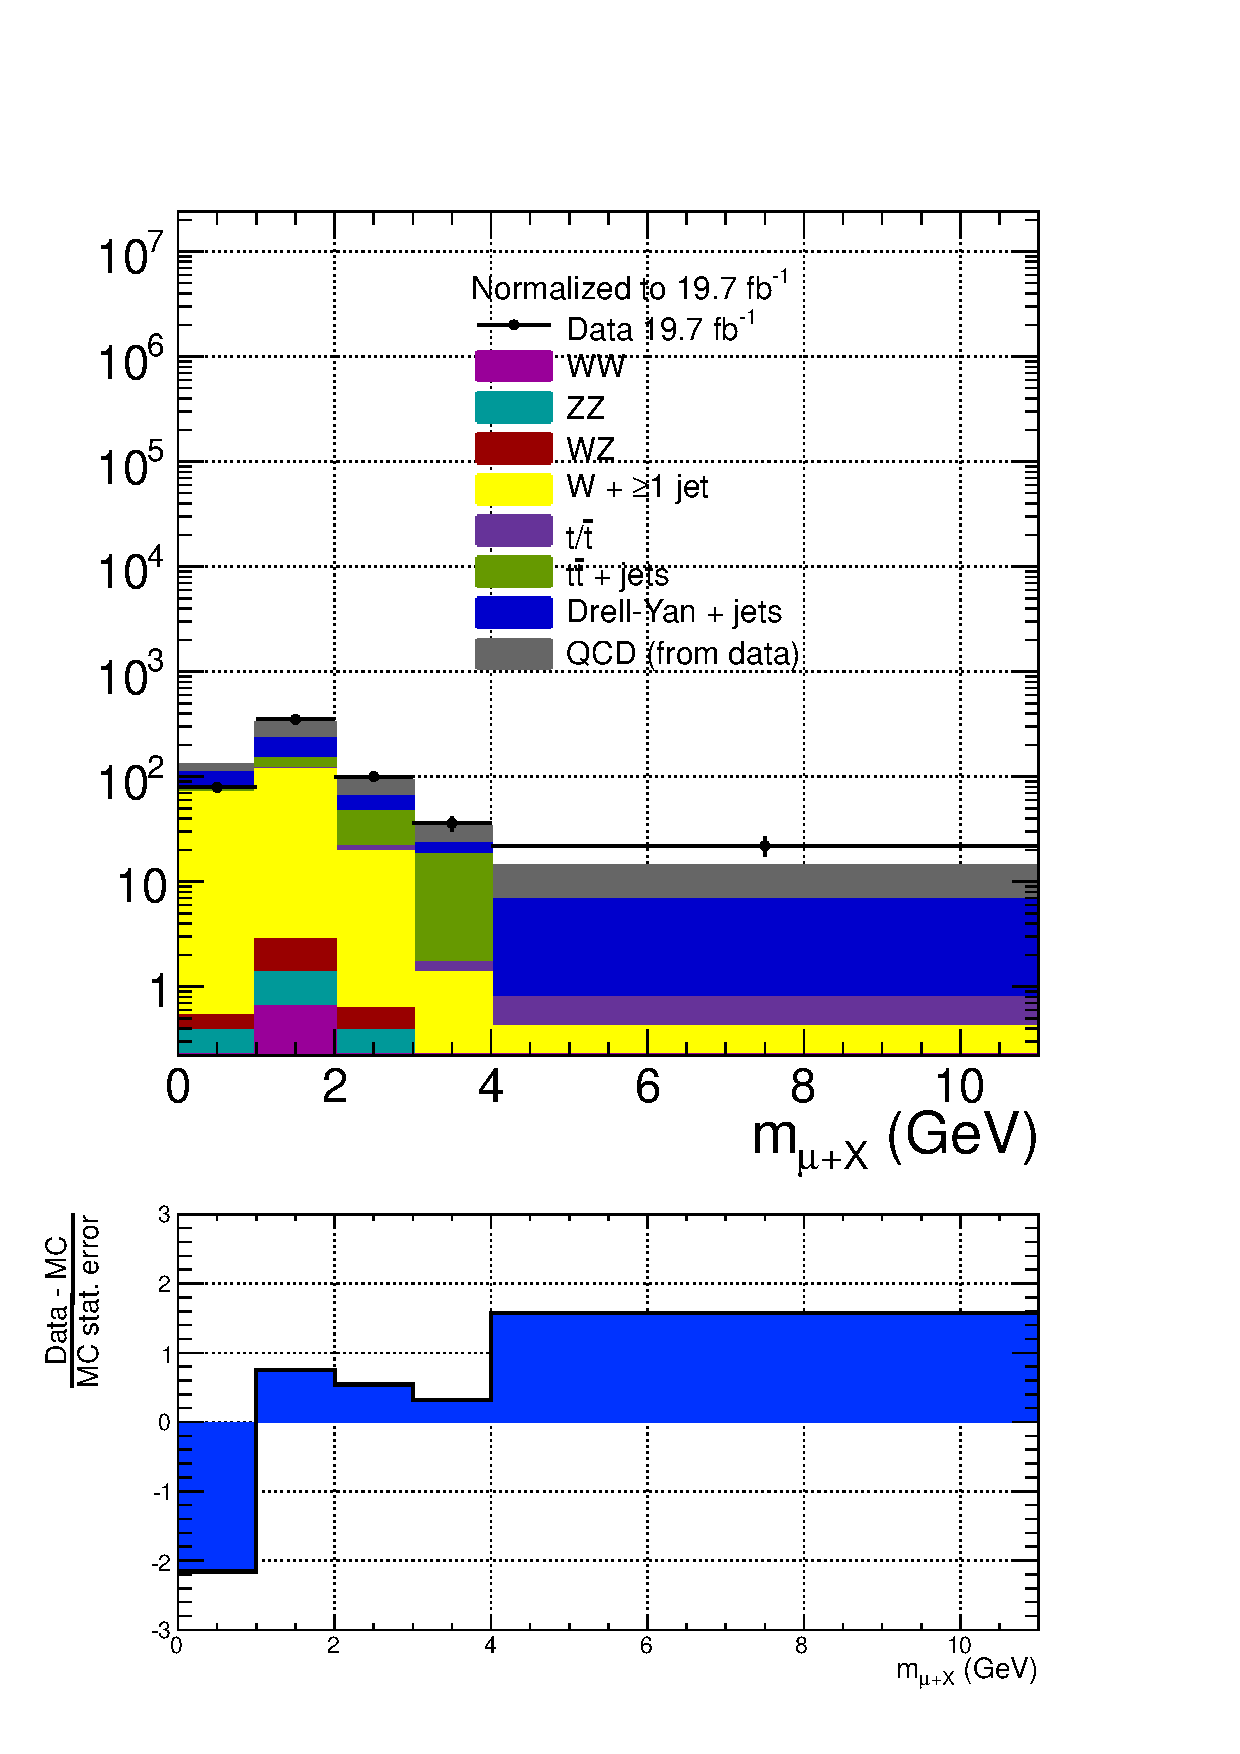
\includegraphics[width=\cmsFigWidth]{figures/dataVsMCQCD_muHadMass_lowMT_v87}
    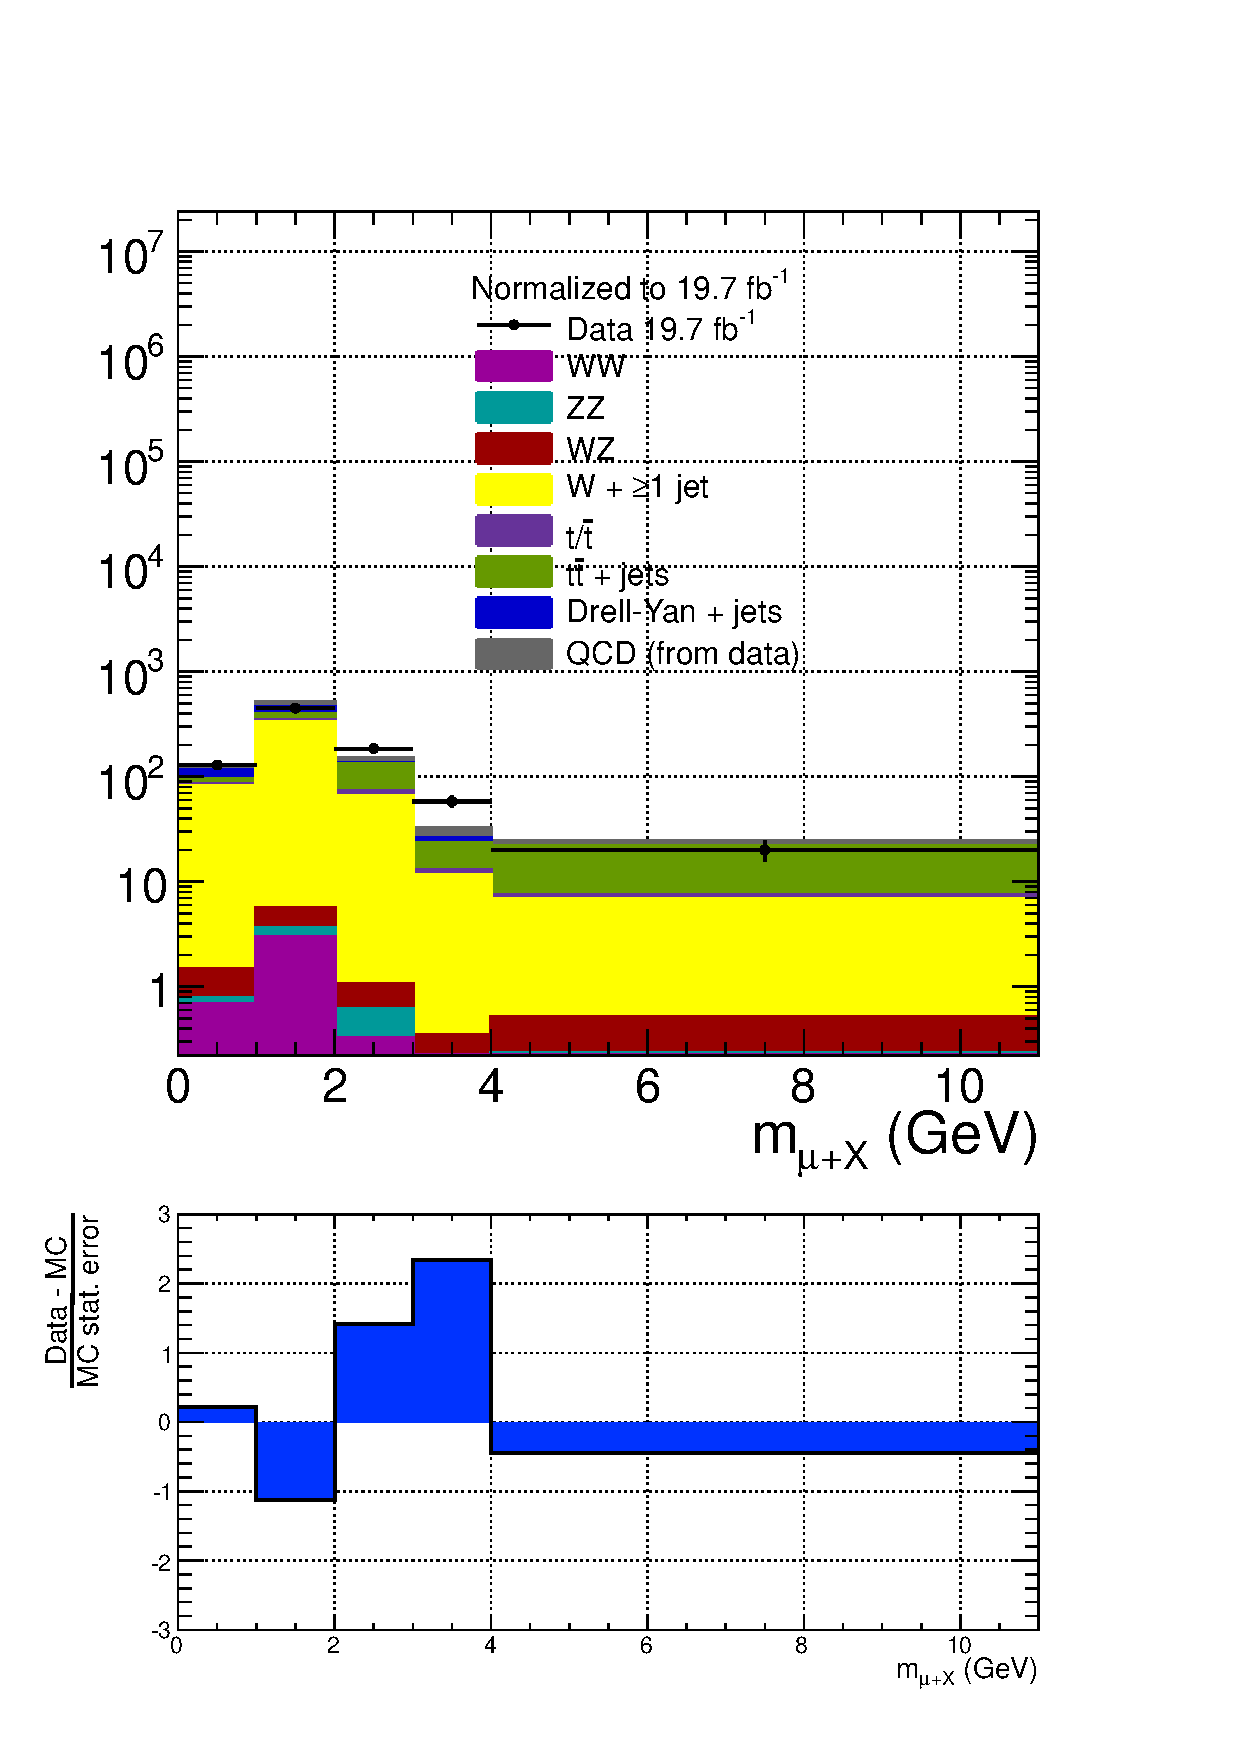
\includegraphics[width=\cmsFigWidth]{figures/dataVsMCQCD_muHadMass_highMT_v87}
    \caption{$m_{\mu+\text{had}}$ distribution for region B data (black points), region B total non-QCD backgrounds from MC (solid stacked histograms), and the QCD prediction from region D data (solid gray histogram).  Errors are statistical only. (\cmsLeft) Low-$M_{\text{T}}$ bin. (\cmsRight) High-$M_{\text{T}}$ bin.}
    \label{fig:regB-data-MC-muHadMass}
  \end{center}
\end{figure}

\begin{figure}[hbtp]
  \begin{center}
    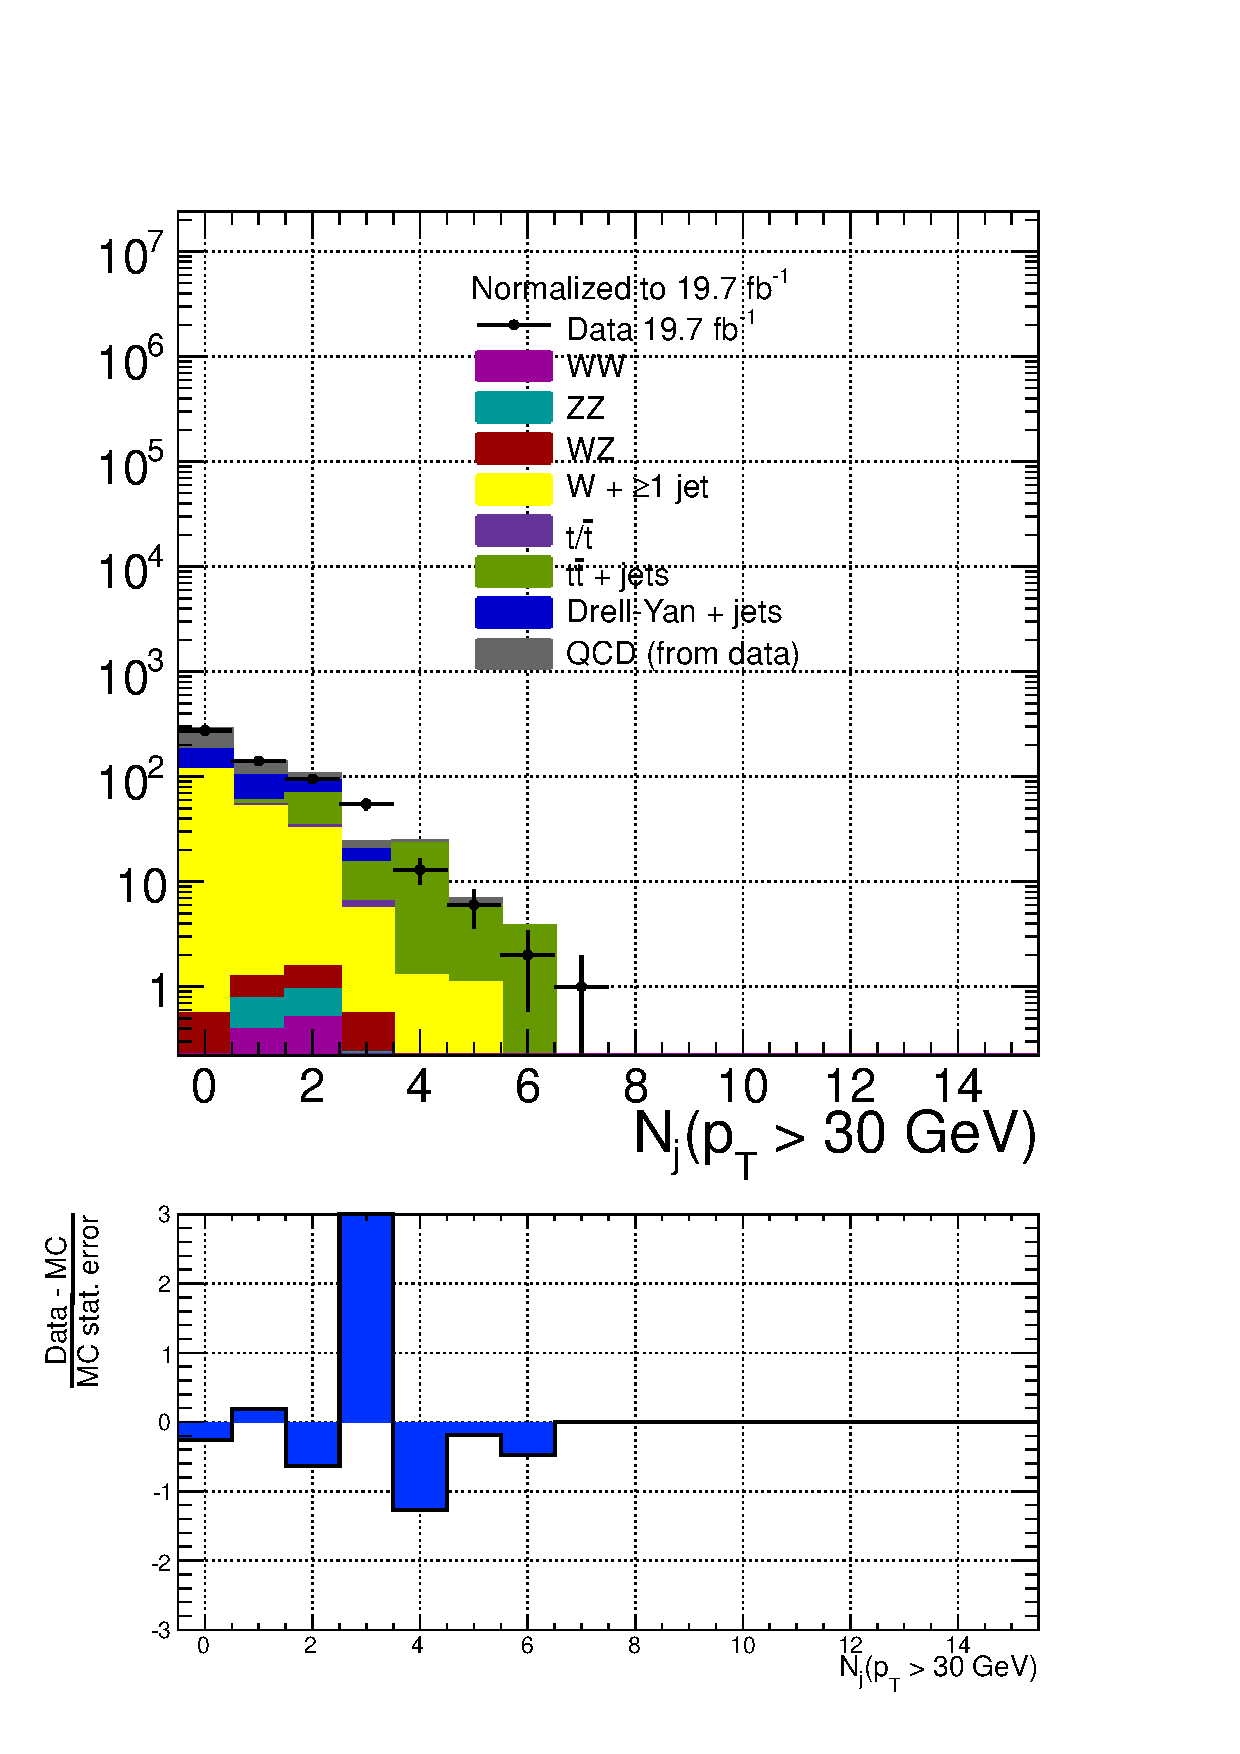
\includegraphics[width=\cmsFigWidth]{figures/dataVsMCQCD_nAddlJetsPTGeq30_lowMT_v87}
    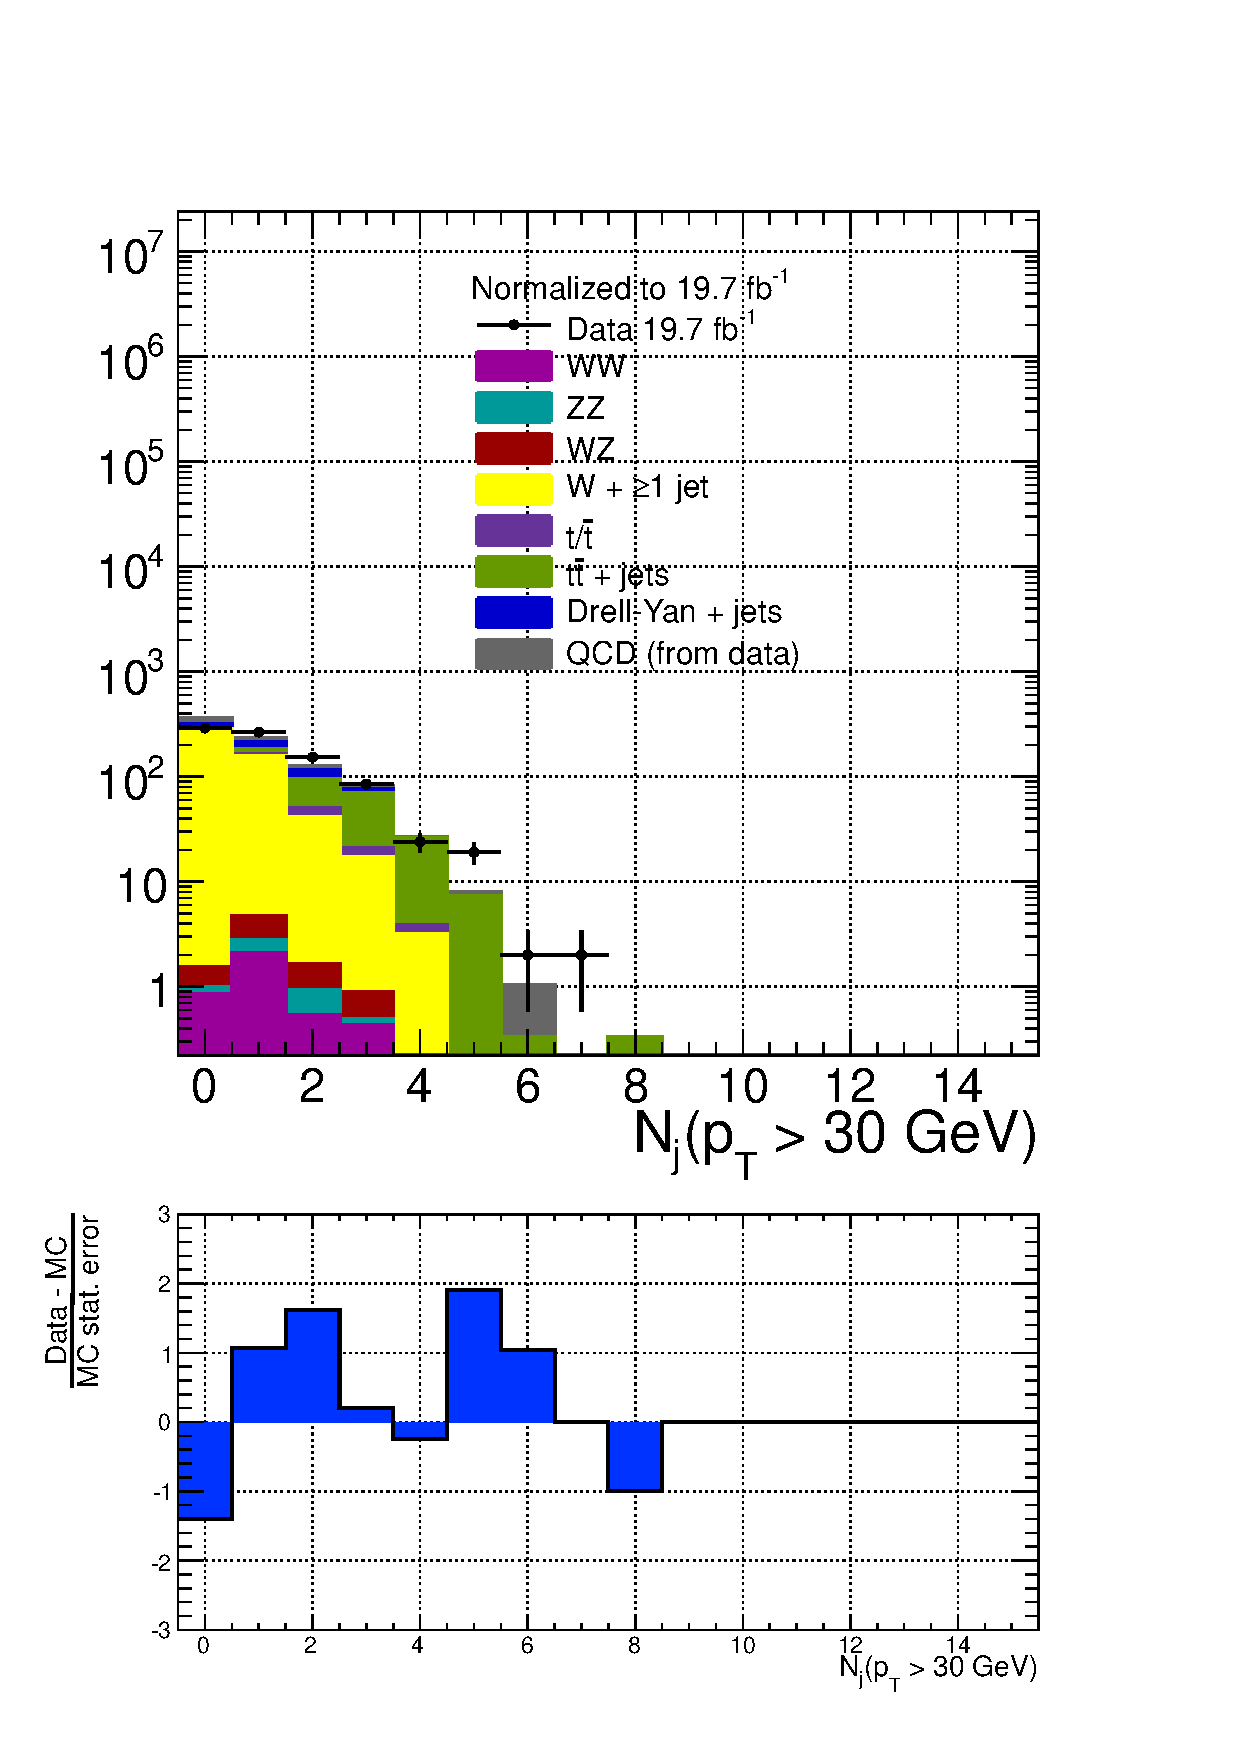
\includegraphics[width=\cmsFigWidth]{figures/dataVsMCQCD_nAddlJetsPTGeq30_highMT_v87}
    \caption{Number of anti-\kt R = 0.5 PF jets with L1FastL2L3~\cite{1748-0221-6-11-P11002} corrected $p_T >$ 30 GeVc. Distribution for region B data (black points), region B total non-QCD backgrounds from MC (solid stacked histograms), and the QCD prediction from region D data (solid gray histogram).  Errors are statistical only. (\cmsLeft) Low-$M_{\text{T}}$ bin. (\cmsRight) High-$M_{\text{T}}$ bin.}
    \label{fig:regB-data-MC-nAddlJetsPTGeq20}
  \end{center}
\end{figure}

\begin{figure}[hbtp]
  \begin{center}
    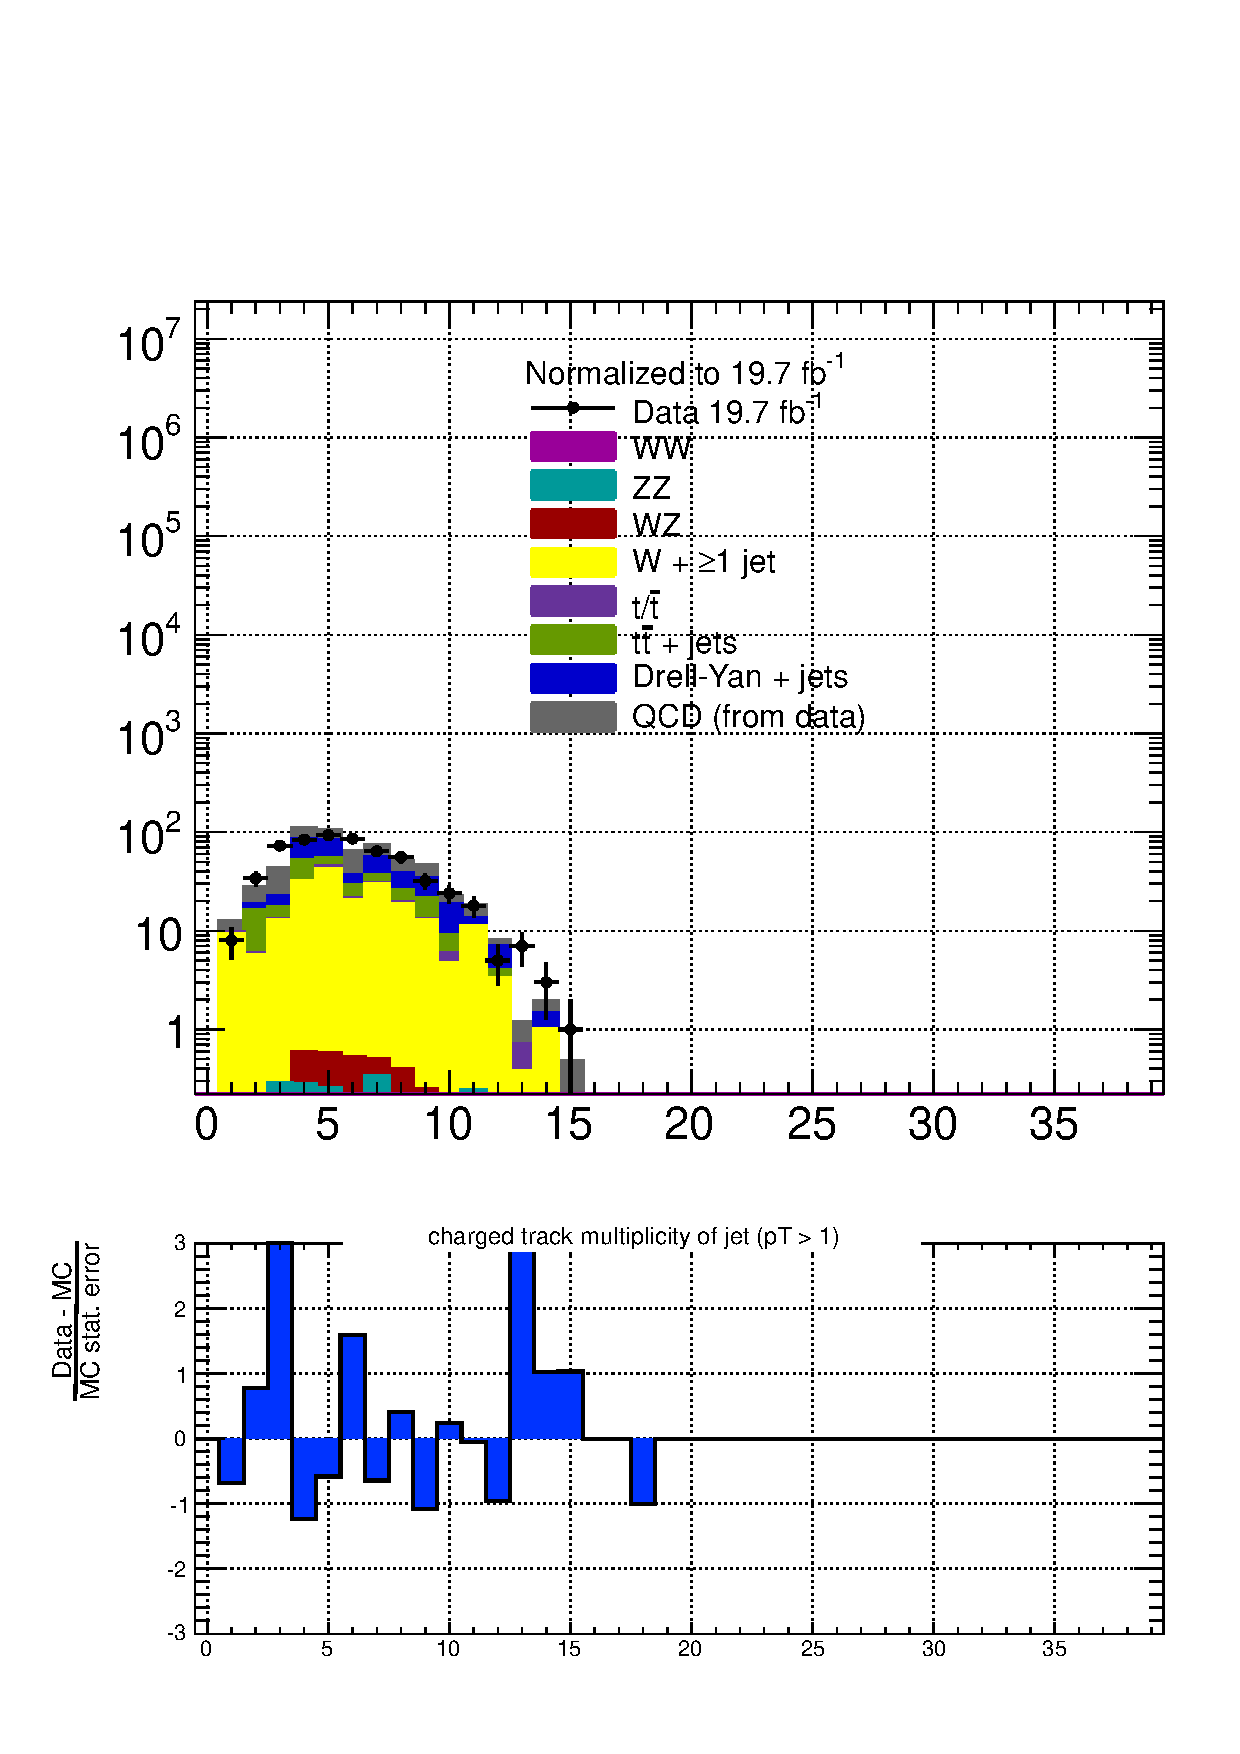
\includegraphics[width=\cmsFigWidth]{figures/dataVsMCQCD_muHadNchtrk1_lowMT_v87}
    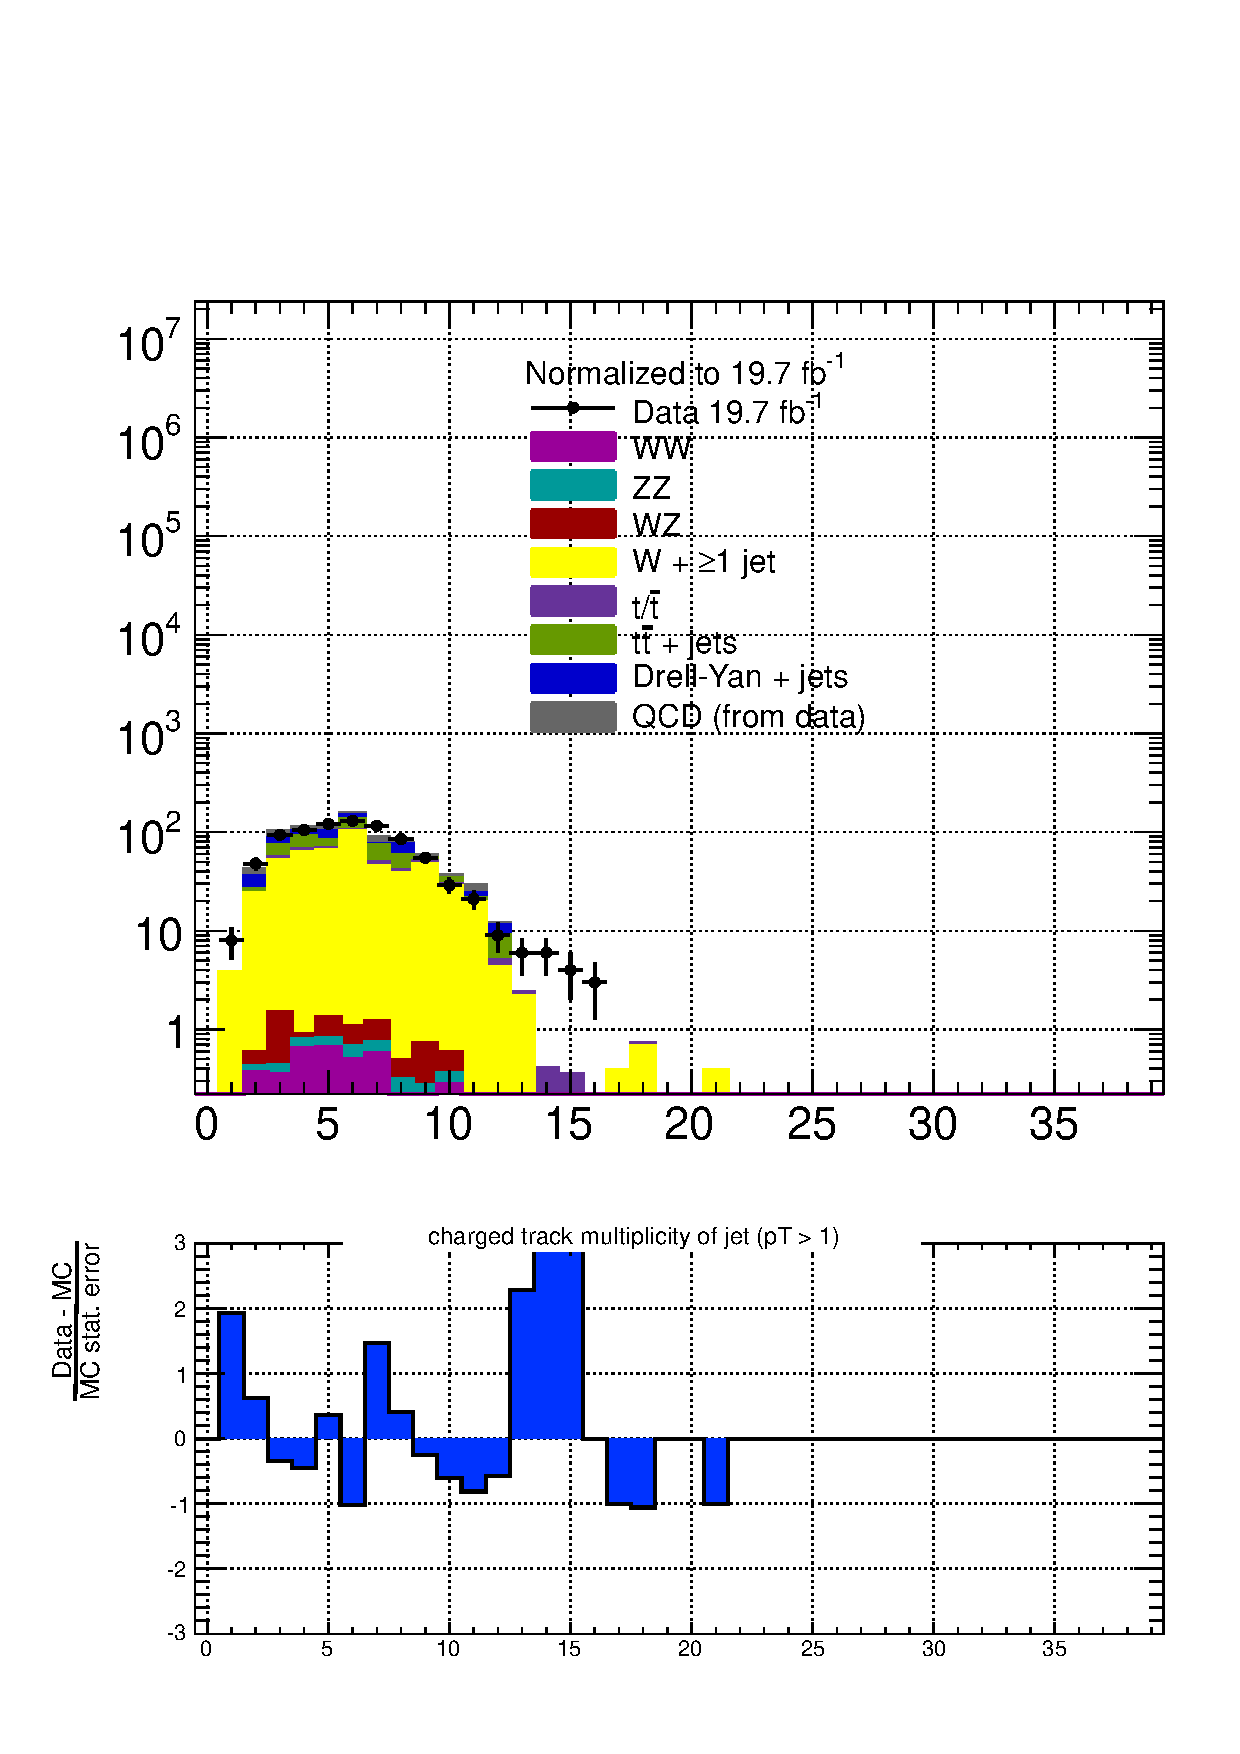
\includegraphics[width=\cmsFigWidth]{figures/dataVsMCQCD_muHadNchtrk1_highMT_v87}
    \caption{Number of charged tracks with $p_T >$ 1 GeVc in the parent jet of the $\tau_{\mu}\tau_{\text{had}}$ object. Distribution for region B data (black points), region B total non-QCD backgrounds from MC (solid stacked histograms), and the QCD prediction from region D data (solid gray histogram).  Errors are statistical only. (\cmsLeft) Low-$M_{\text{T}}$ bin. (\cmsRight) High-$M_{\text{T}}$ bin.}
    \label{fig:regB-data-MC-muHadNchtrk1}
  \end{center}
\end{figure}

\begin{figure}[hbtp]
  \begin{center}
    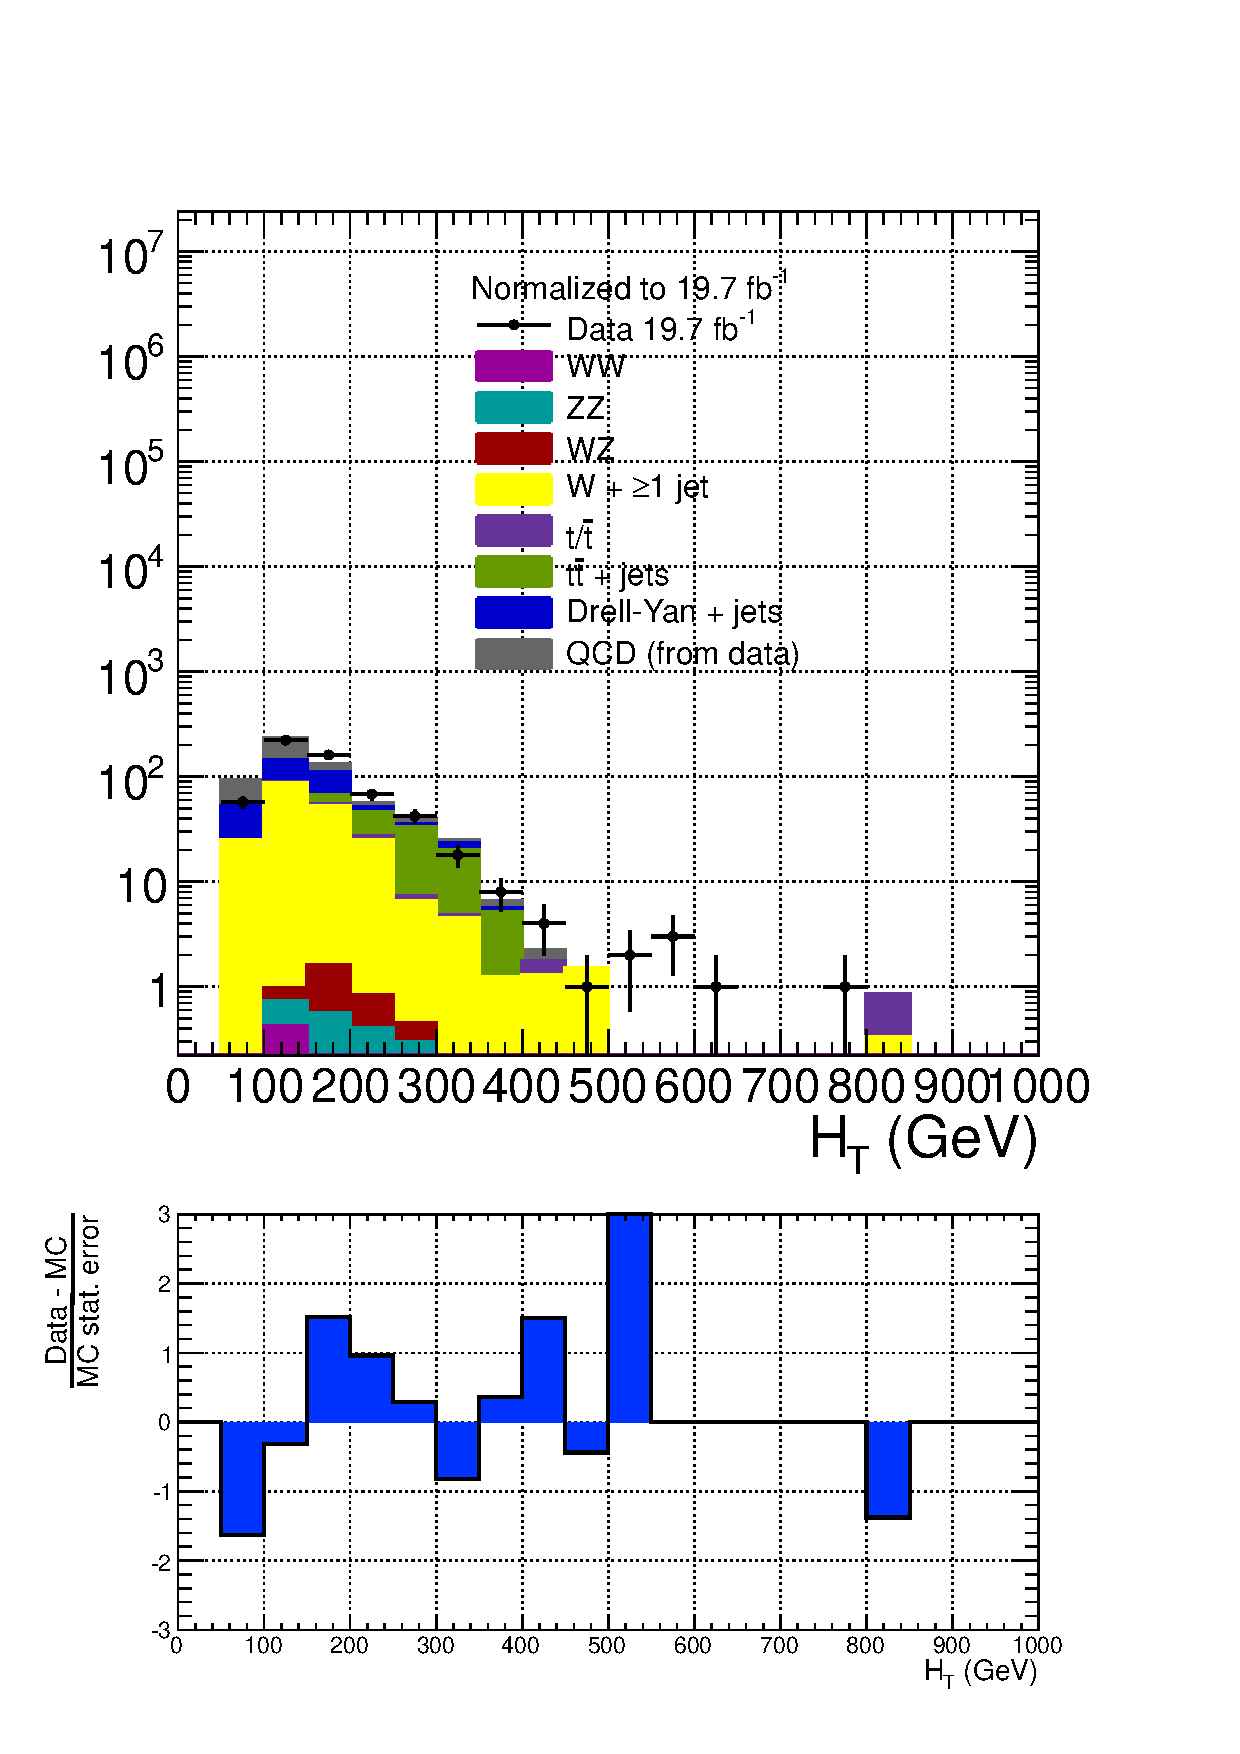
\includegraphics[width=\cmsFigWidth]{figures/dataVsMCQCD_HT_lowMT_v87}
    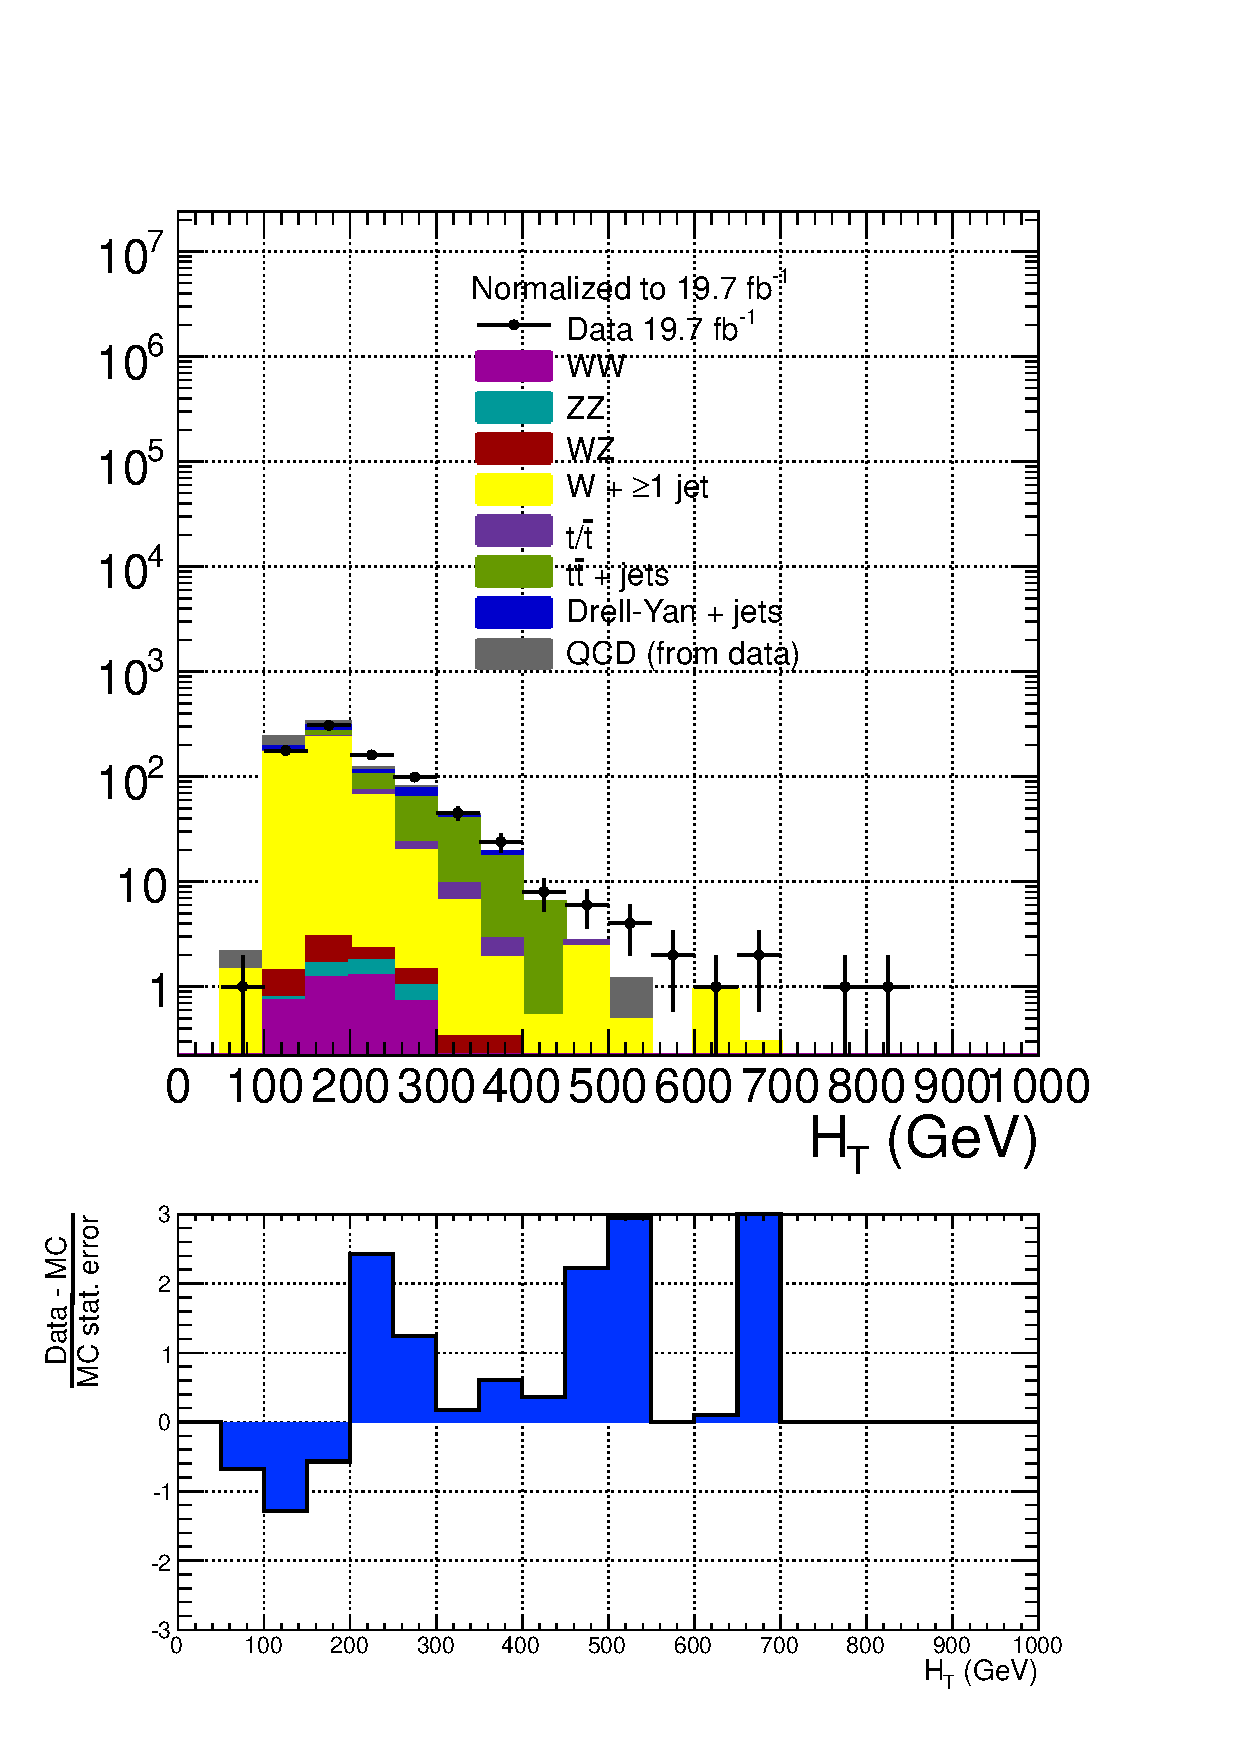
\includegraphics[width=\cmsFigWidth]{figures/dataVsMCQCD_HT_highMT_v87}
    \caption{$p_T$ sum of the tau muon, hadronic tau, highest $p_T$ distinct jet, trigger muon, and \ETslash. Distribution for region B data (black points), region B total non-QCD backgrounds from MC (solid stacked histograms), and the QCD prediction from region D data (solid gray histogram).  Errors are statistical only. (\cmsLeft) Low-$M_{\text{T}}$ bin. (\cmsRight) High-$M_{\text{T}}$ bin.}
    \label{fig:regB-data-MC-tauMuTauHadJetWMuMETHT}
  \end{center}
\end{figure}

\begin{figure}[hbtp]
  \begin{center}
    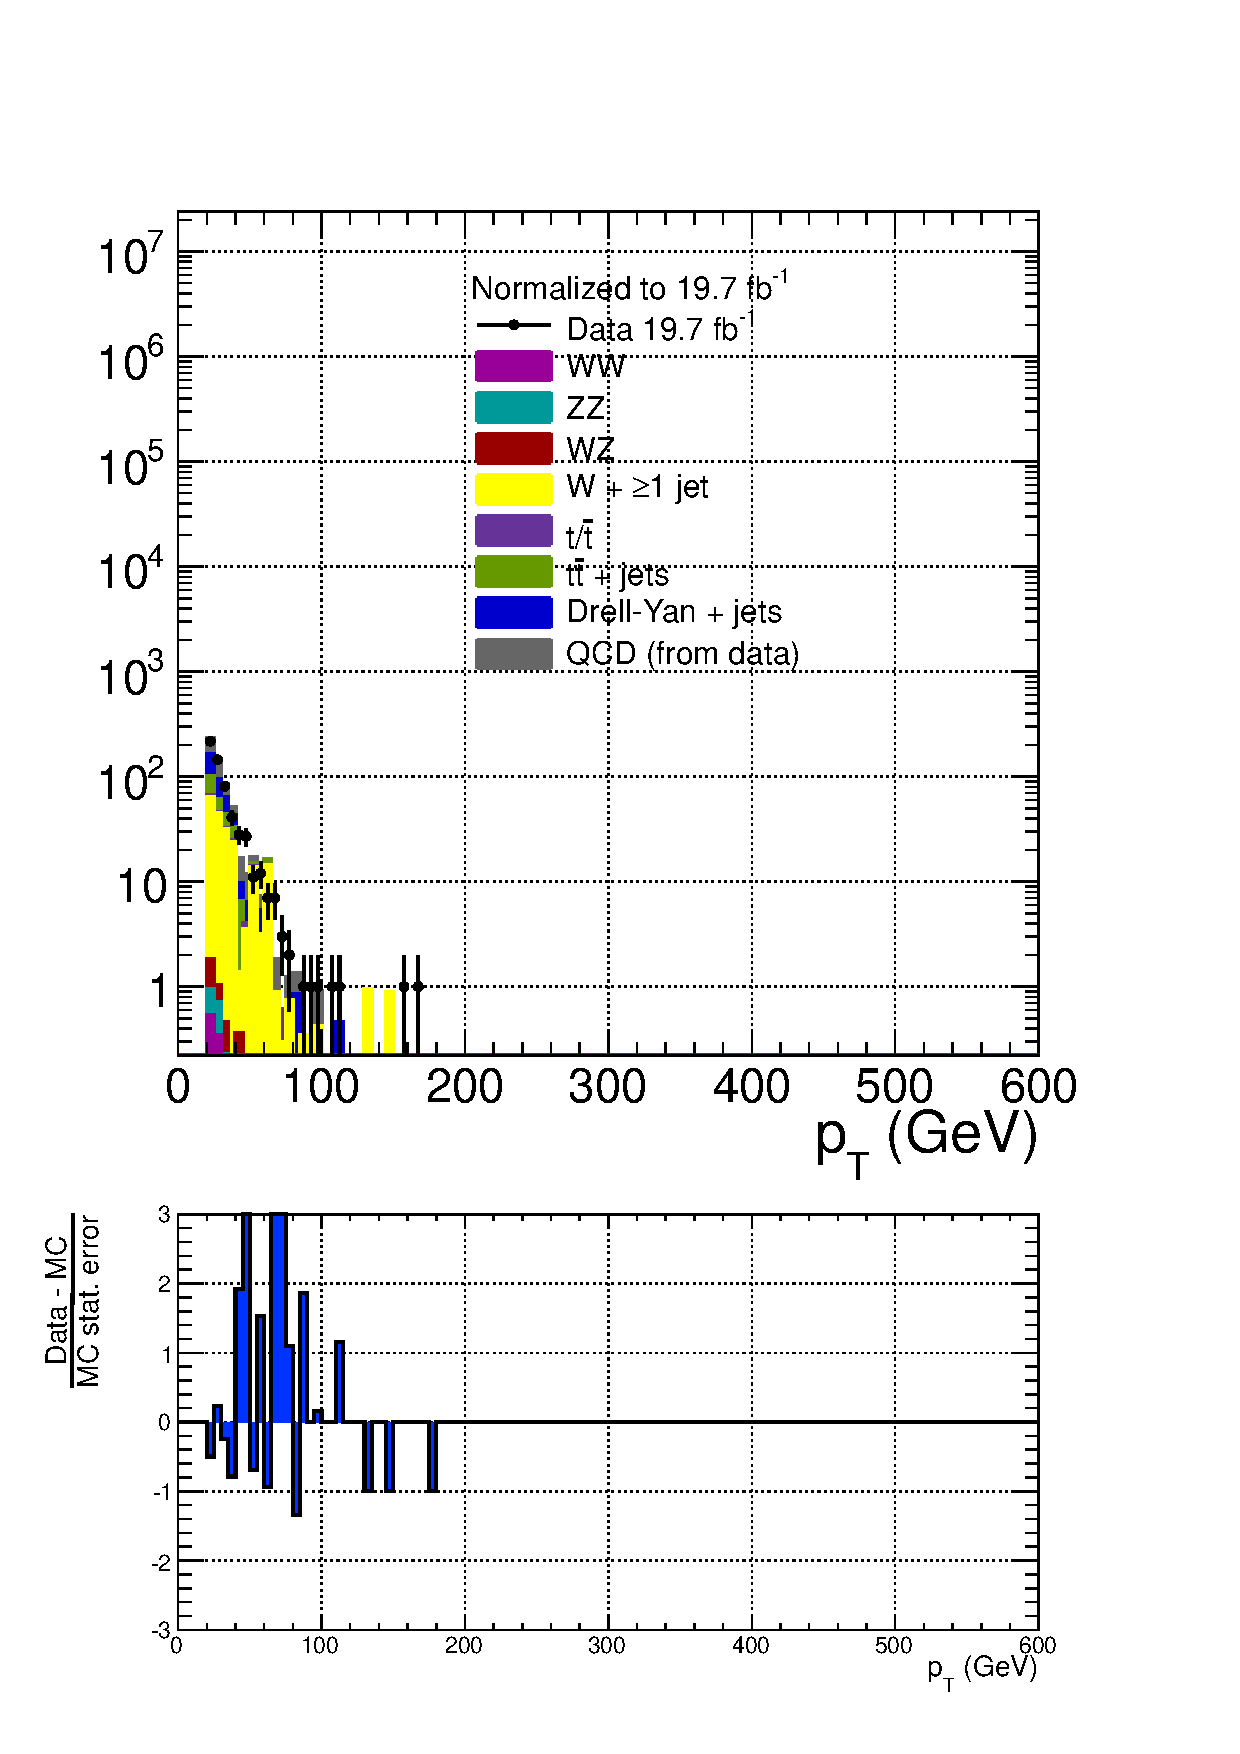
\includegraphics[width=\cmsFigWidth]{figures/dataVsMCQCD_tauHadPT_lowMT_v87}
    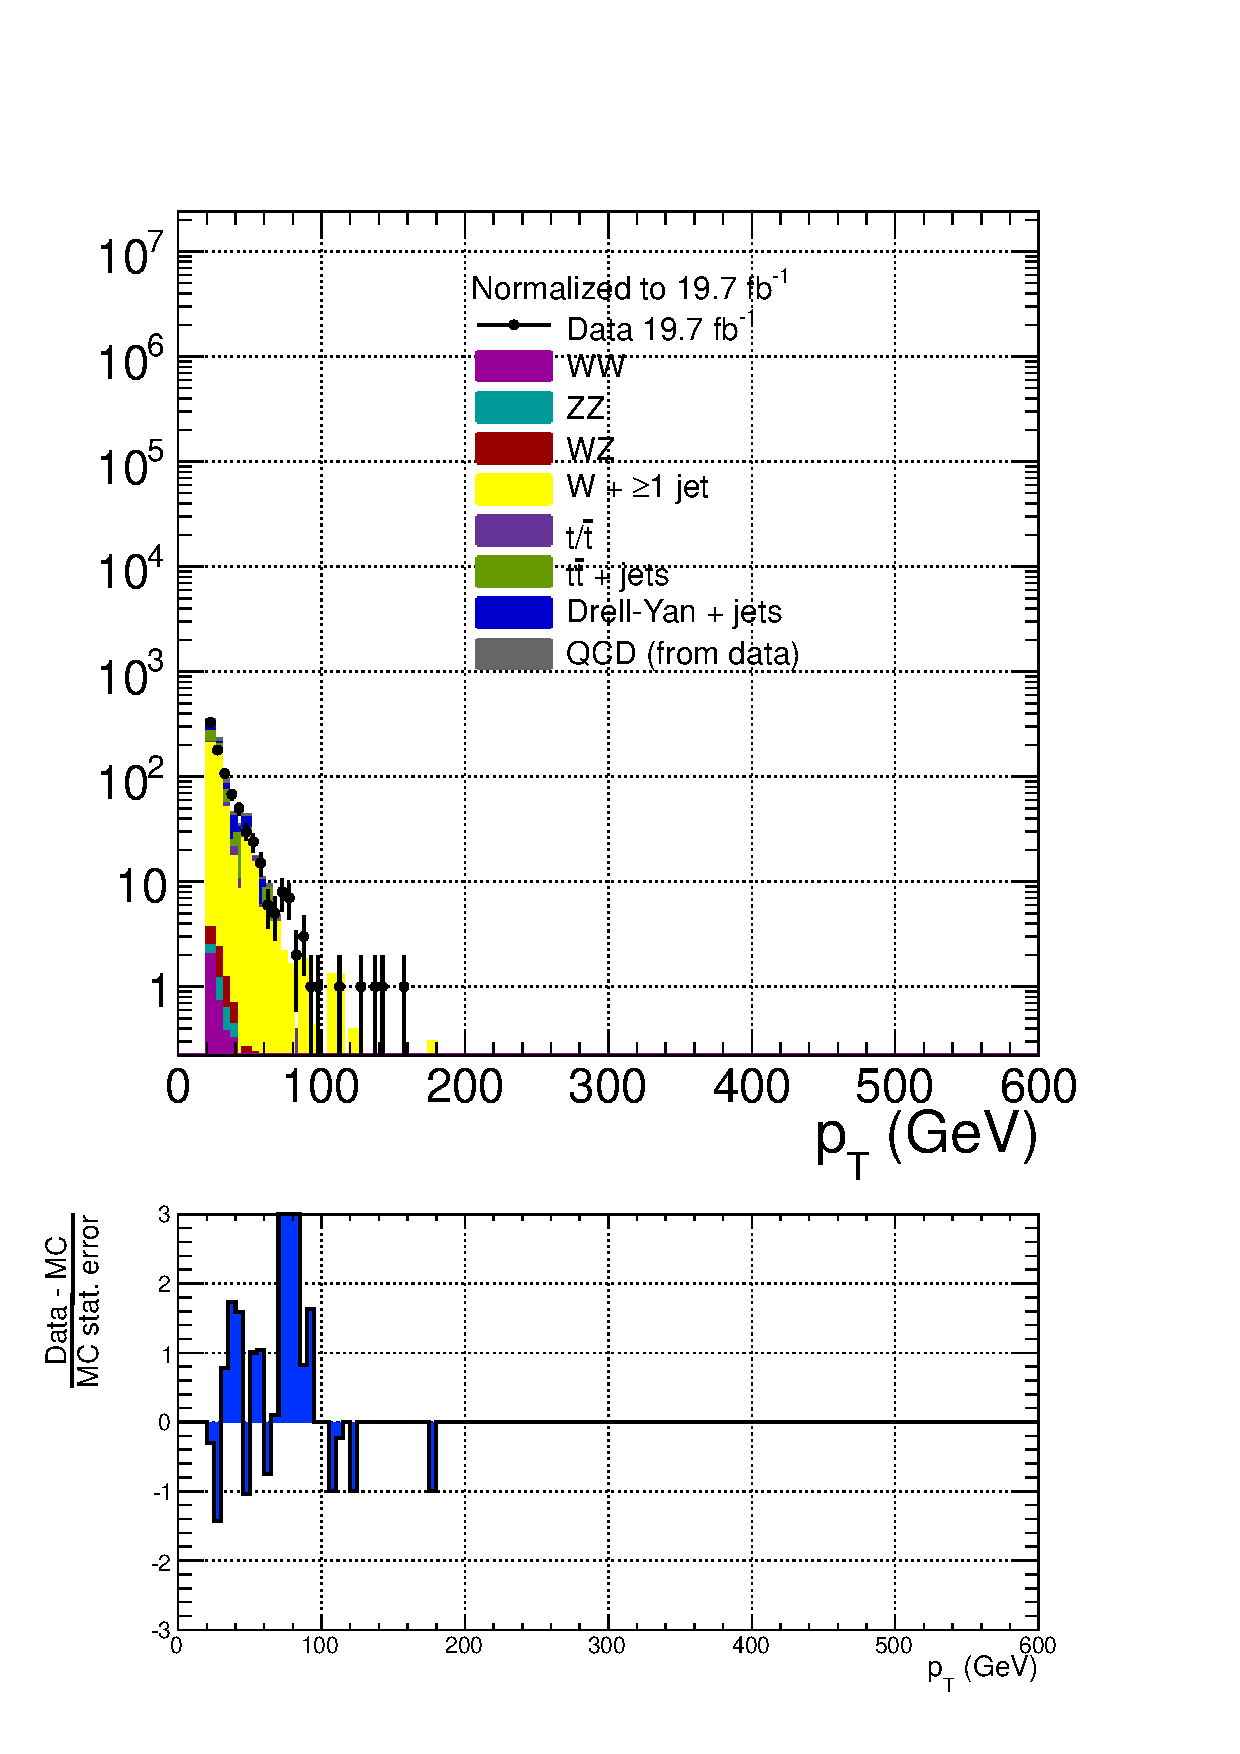
\includegraphics[width=\cmsFigWidth]{figures/dataVsMCQCD_tauHadPT_highMT_v87}
   \caption{Hadronic tau $p_T$ distribution for region B data (black points), region B total non-QCD backgrounds from MC (solid stacked histograms), and the QCD prediction from region D data (solid gray histogram).  Errors are statistical only. (\cmsLeft) Low-$M_{\text{T}}$ bin. (\cmsRight) High-$M_{\text{T}}$ bin.}
    \label{fig:regB-data-MC-tauHadPT}
  \end{center}
\end{figure}

\begin{figure}[hbtp]
  \begin{center}
    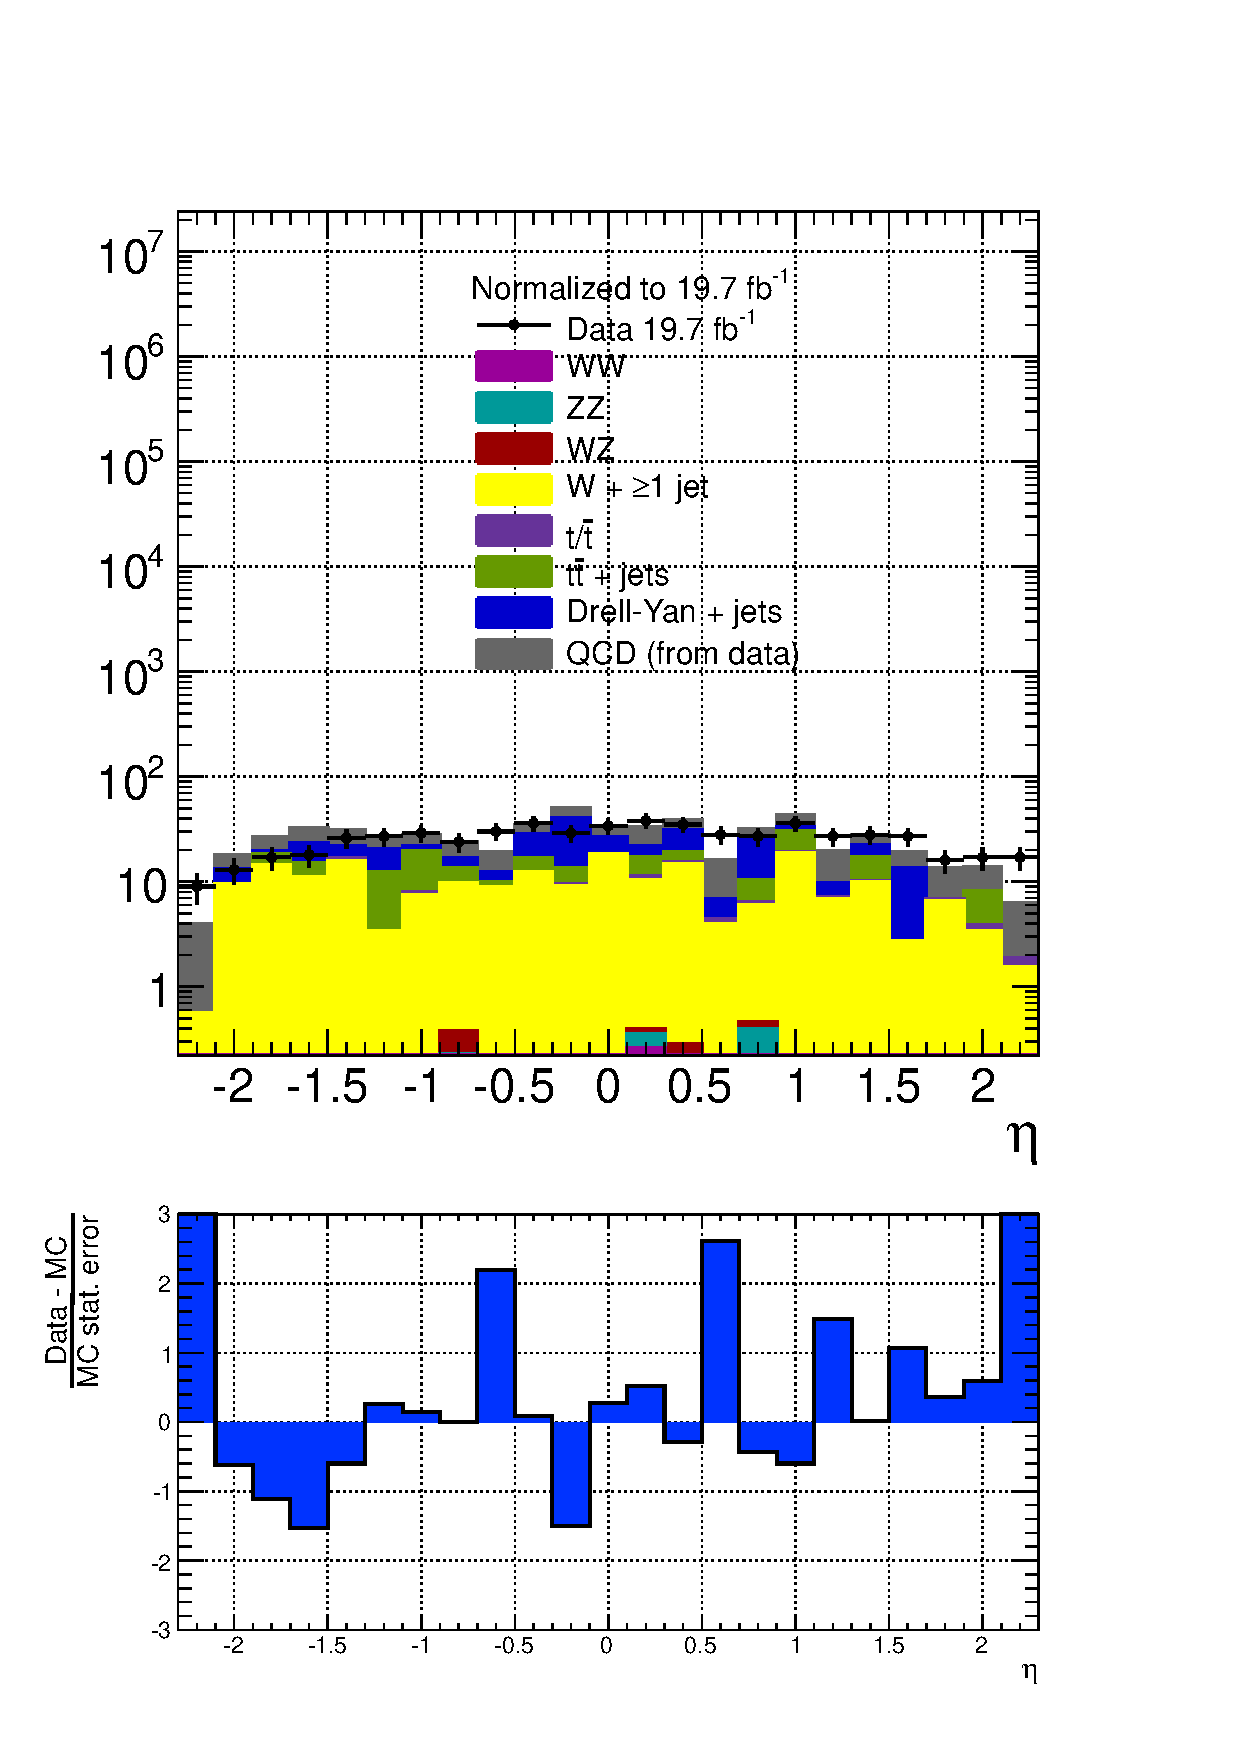
\includegraphics[width=\cmsFigWidth]{figures/dataVsMCQCD_tauHadEta_lowMT_v87}
    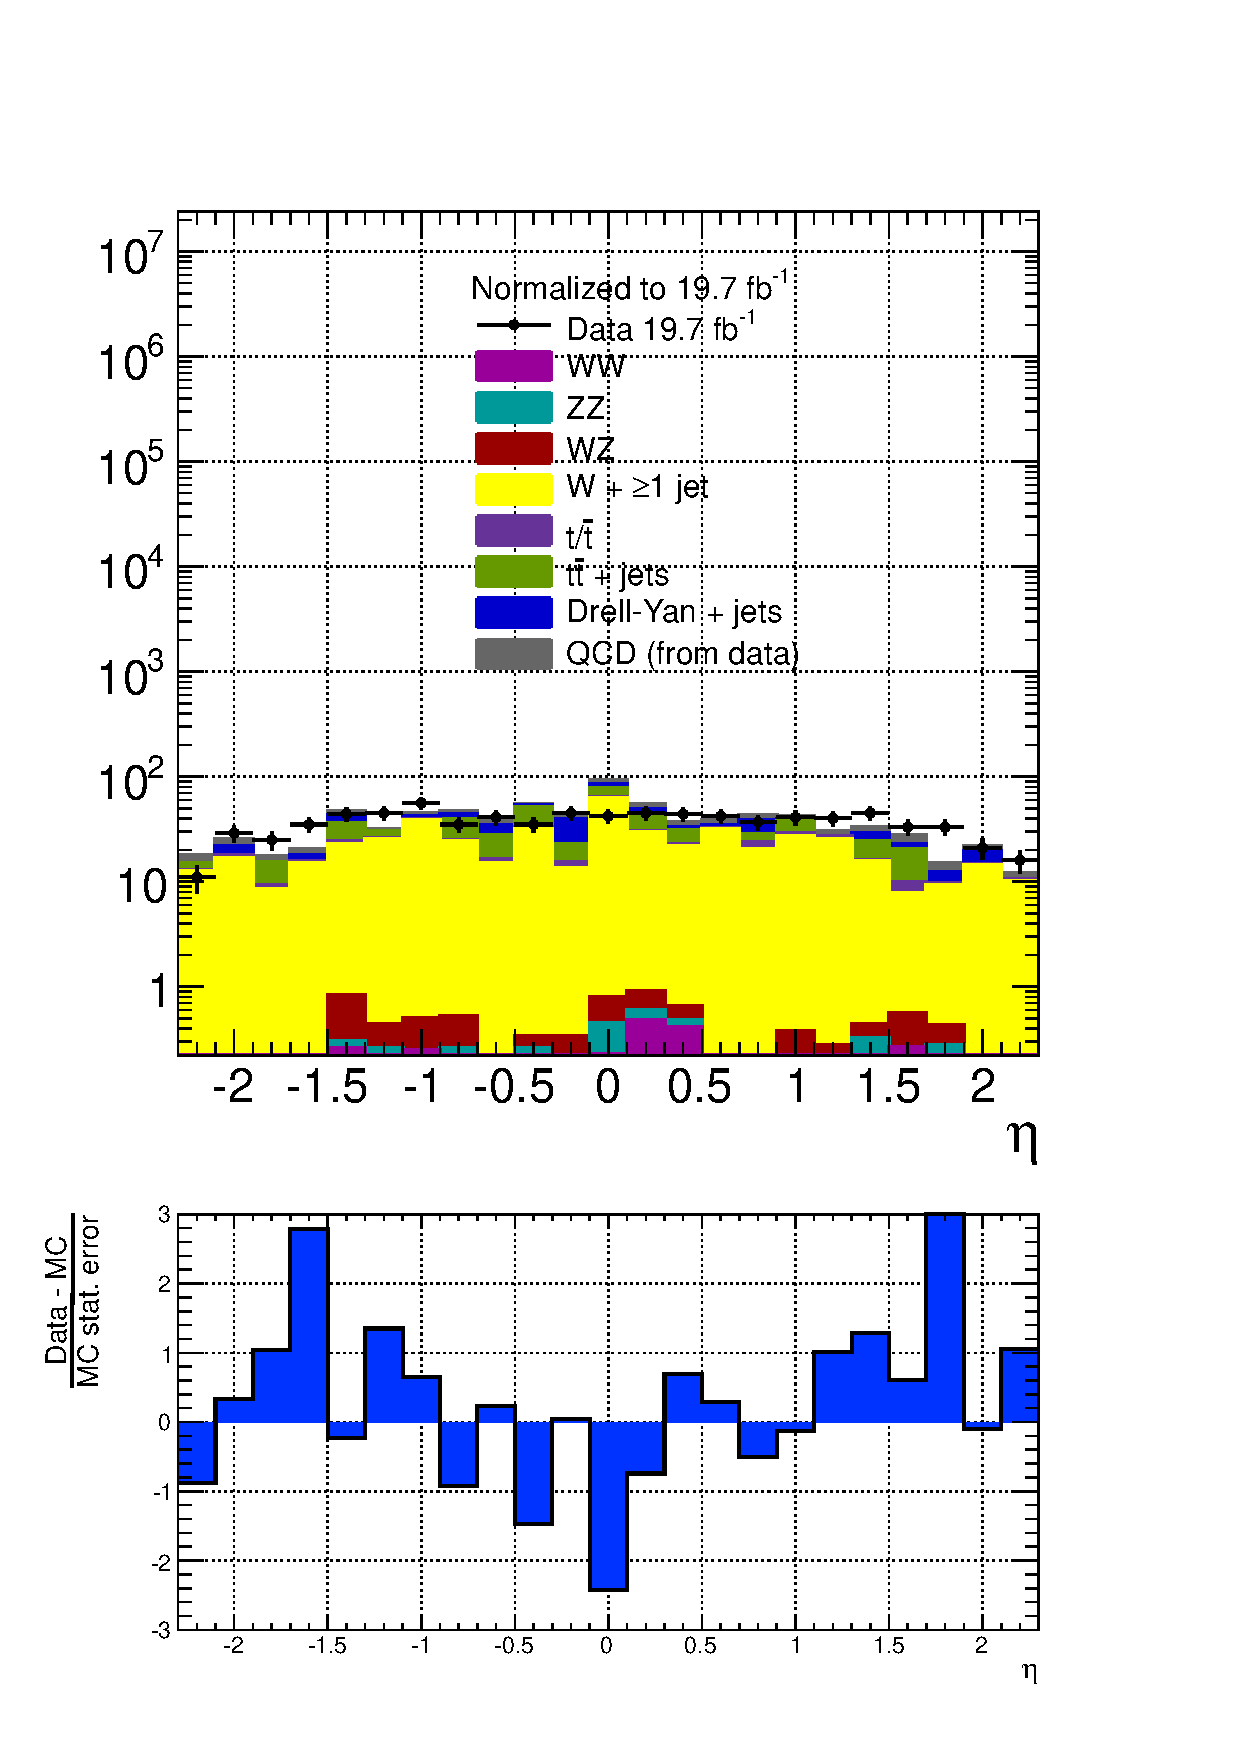
\includegraphics[width=\cmsFigWidth]{figures/dataVsMCQCD_tauHadEta_highMT_v87}
    \caption{Hadronic tau $\eta$ distribution for region B data (black points), region B total non-QCD backgrounds from MC (solid stacked histograms), and the QCD prediction from region D data (solid gray histogram).  Errors are statistical only. (\cmsLeft) Low-$M_{\text{T}}$ bin. (\cmsRight) High-$M_{\text{T}}$ bin.}
    \label{fig:regB-data-MC-tauHadEta}
  \end{center}
\end{figure}

\begin{figure}[hbtp]
  \begin{center}
    \includegraphics[width=\cmsFigWidth]{figures/dataVsMCQCD_tauHadIso_lowMT_v87}
    \includegraphics[width=\cmsFigWidth]{figures/dataVsMCQCD_tauHadIso_highMT_v87}
    \caption{Hadronic tau isolation distribution for region B data (black points), region B total non-QCD backgrounds from MC (solid stacked histograms), and the QCD prediction from region D data (solid gray histogram).  Errors are statistical only. (\cmsLeft) Low-$M_{\text{T}}$ bin. (\cmsRight) High-$M_{\text{T}}$ bin.}
    \label{fig:regB-data-MC-tauHadIso}
  \end{center}
\end{figure}

\begin{figure}[hbtp]
  \begin{center}
    \includegraphics[width=\cmsFigWidth]{figures/dataVsMCQCD_tauHadDecayMode_lowMT_v87}
    \includegraphics[width=\cmsFigWidth]{figures/dataVsMCQCD_tauHadDecayMode_highMT_v87}
    \caption{Hadronic tau decay mode distribution for region B data (black points), region B total non-QCD backgrounds from MC (solid stacked histograms), and the QCD prediction from region D data (solid gray histogram).  Errors are statistical only. (\cmsLeft) Low-$M_{\text{T}}$ bin. (\cmsRight) High-$M_{\text{T}}$ bin.}
    \label{fig:regB-data-MC-tauHadDecayMode}
  \end{center}
\end{figure}

\begin{figure}[hbtp]
  \begin{center}
    \includegraphics[width=\cmsFigWidth]{figures/dataVsMCQCD_CSV_lowMT_v87}
    \includegraphics[width=\cmsFigWidth]{figures/dataVsMCQCD_CSV_highMT_v87}
    \caption{CSV discriminant distribution for region B data (black points), region B total non-QCD backgrounds from MC (solid stacked histograms), and the QCD prediction from region D data (solid gray histogram).  Errors are statistical only. (\cmsLeft) Low-$M_{\text{T}}$ bin. (\cmsRight) High-$M_{\text{T}}$ bin.}
    \label{fig:regB-data-MC-bTagDiscrim}
  \end{center}
\end{figure}

\clearpage

\begin{figure}[hbtp]
  \begin{center}
    \includegraphics[width=\cmsFigWidth]{figures/dataVsMCQCD_tauMuPT_lowMT_v87}
    \includegraphics[width=\cmsFigWidth]{figures/dataVsMCQCD_tauMuPT_highMT_v87}
    \caption{$\tau$ muon $p_T$ distribution for region B data (black points), region B total non-QCD backgrounds from MC (solid stacked histograms), and the QCD prediction from region D data (solid gray histogram).  Errors are statistical only. (\cmsLeft) Low-$M_{\text{T}}$ bin. (\cmsRight) High-$M_{\text{T}}$ bin.}
    \label{fig:regB-data-MC-tauMuPT}
  \end{center}
\end{figure}

%Subsection: final bkg and uncertainties
\subsection{Final jet fake background prediction and systematic uncertainties\label{sec:bkgs-jet-fake-unc}}

The region B data sample contains some mixture of Drell-Yan, $W$ + jets, $t\bar{t}$ and single top, QCD di-jet, and diboson backgrounds.  The low-$M_{\text{T}}$ bin is dominated by QCD and Drell-Yan, while the high-$M_{\text{T}}$ bin is dominated by $W$ + jets and $t\bar{t}$.  Within each bin, MC predicts the background composition in regions B and A to be reasonably similar, as shown in Table~\ref{tab:MC-breakdown}.  Furthermore, the shape of the $m_{\mu+\text{had}}$ distribution for each individual background component is predicted to be similar in regions A and B, as shown in Figs.~\ref{fig:MC-regA-vs-regB-main-lowMT}-\ref{fig:MC-regA-vs-regB-secondary-highMT}.  However, the lack of exact knowledge of the background composition of regions A and B (i.e., the relative ratios of each individual background source), coupled with small differences between the $m_{\mu+\text{had}}$ distributions for each background, constitute the main systematic uncertainty of the method.

\begin{sidewaystable}
%\begin{table*}[htbH]
\begin{center}
\caption{Expected events below $m_{\mu+\text{had}}$ = 2 GeV and above $m_{\mu+\text{had}}$ = 4 GeV in Regions B and A.  The MC backgrounds are normalized to 19.7 fb$^{-1}$.  The QCD normalization is given by Eqs.~\ref{eq:f-B-QCD} and~\ref{eq:R-B-QCD} for region B and~\ref{eq:f-A-QCD} and~\ref{eq:R-A-QCD} for region A.  The number in parentheses is the percentage of the total.\label{tab:MC-breakdown}}
\singlespacing
\resizebox{\textwidth}{!}{\begin{tabular}{l|llll|llll}
\hline \multicolumn{1}{c}{} & \multicolumn{4}{c}{$\text{M}_{\text{T}}$ $\le$ 50 GeV} & \multicolumn{4}{c}{$\text{M}_{\text{T}}$ $>$ 50 GeV} \\
\multicolumn{1}{c}{} & \multicolumn{2}{c}{Region A} & \multicolumn{2}{c}{Region B} & \multicolumn{2}{c}{Region A} & \multicolumn{2}{c}{Region B} \\
\multicolumn{1}{l}{$m_{\mu+\text{had}}$} & $<$ 2 GeV & $\geq$ 4 GeV & $<$ 2 GeV & \multicolumn{1}{l}{$\geq$ 4 GeV} & $<$ 2 GeV & $\geq$ 4 GeV & $<$ 2 GeV & $\geq$ 4 GeV \\
\hline
\hline
WW & \begin{tabular}[c]{@{}l@{}}0.315 $\pm$ 0.18 \\(0.3\%)\end{tabular} & \begin{tabular}[c]{@{}l@{}}0 $\pm$ 0 \\(0\%)\end{tabular} & \begin{tabular}[c]{@{}l@{}}0.726 $\pm$ 0.3 \\(0.16\%)\end{tabular} & \begin{tabular}[c]{@{}l@{}}0 $\pm$ 0 \\(0\%)\end{tabular} & \begin{tabular}[c]{@{}l@{}}0.472 $\pm$ 0.24 \\(0.38\%)\end{tabular} & \begin{tabular}[c]{@{}l@{}}0 $\pm$ 0 \\(0\%)\end{tabular} & \begin{tabular}[c]{@{}l@{}}3.66 $\pm$ 0.68 \\(0.58\%)\end{tabular} & \begin{tabular}[c]{@{}l@{}}0 $\pm$ 0 \\(0\%)\end{tabular} \\
\hline
ZZ & \begin{tabular}[c]{@{}l@{}}0.262 $\pm$ 0.096 \\(0.25\%)\end{tabular} & \begin{tabular}[c]{@{}l@{}}0.108 $\pm$ 0.062 \\(1\%)\end{tabular} & \begin{tabular}[c]{@{}l@{}}0.998 $\pm$ 0.2 \\(0.22\%)\end{tabular} & \begin{tabular}[c]{@{}l@{}}0.0421 $\pm$ 0.042 \\(0.3\%)\end{tabular} & \begin{tabular}[c]{@{}l@{}}0.263 $\pm$ 0.1 \\(0.21\%)\end{tabular} & \begin{tabular}[c]{@{}l@{}}0.145 $\pm$ 0.085 \\(4.4\%)\end{tabular} & \begin{tabular}[c]{@{}l@{}}0.723 $\pm$ 0.17 \\(0.11\%)\end{tabular} & \begin{tabular}[c]{@{}l@{}}0.235 $\pm$ 0.097 \\(0.97\%)\end{tabular} \\
\hline
WZ & \begin{tabular}[c]{@{}l@{}}0.344 $\pm$ 0.15 \\(0.33\%)\end{tabular} & \begin{tabular}[c]{@{}l@{}}0 $\pm$ 0 \\(0\%)\end{tabular} & \begin{tabular}[c]{@{}l@{}}1.58 $\pm$ 0.35 \\(0.35\%)\end{tabular} & \begin{tabular}[c]{@{}l@{}}0 $\pm$ 0 \\(0\%)\end{tabular} & \begin{tabular}[c]{@{}l@{}}1.08 $\pm$ 0.28 \\(0.86\%)\end{tabular} & \begin{tabular}[c]{@{}l@{}}0.404 $\pm$ 0.17 \\(12\%)\end{tabular} & \begin{tabular}[c]{@{}l@{}}2.71 $\pm$ 0.46 \\(0.43\%)\end{tabular} & \begin{tabular}[c]{@{}l@{}}0.276 $\pm$ 0.14 \\(1.1\%)\end{tabular} \\
\hline
W + jets & \begin{tabular}[c]{@{}l@{}}41.1 $\pm$ 10 \\(39\%)\end{tabular} & \begin{tabular}[c]{@{}l@{}}0 $\pm$ 0 \\(0\%)\end{tabular} & \begin{tabular}[c]{@{}l@{}}180 $\pm$ 26 \\(40\%)\end{tabular} & \begin{tabular}[c]{@{}l@{}}0.367 $\pm$ 0.37 \\(2.6\%)\end{tabular} & \begin{tabular}[c]{@{}l@{}}74.6 $\pm$ 14 \\(60\%)\end{tabular} & \begin{tabular}[c]{@{}l@{}}1.76 $\pm$ 1.5 \\(54\%)\end{tabular} & \begin{tabular}[c]{@{}l@{}}409 $\pm$ 39 \\(65\%)\end{tabular} & \begin{tabular}[c]{@{}l@{}}6.29 $\pm$ 2.8 \\(26\%)\end{tabular} \\
\hline
Single top & \begin{tabular}[c]{@{}l@{}}1.56 $\pm$ 0.8 \\(1.5\%)\end{tabular} & \begin{tabular}[c]{@{}l@{}}0.278 $\pm$ 0.28 \\(2.6\%)\end{tabular} & \begin{tabular}[c]{@{}l@{}}4.47 $\pm$ 1.3 \\(0.99\%)\end{tabular} & \begin{tabular}[c]{@{}l@{}}0.373 $\pm$ 0.32 \\(2.7\%)\end{tabular} & \begin{tabular}[c]{@{}l@{}}2.5 $\pm$ 0.86 \\(2\%)\end{tabular} & \begin{tabular}[c]{@{}l@{}}0 $\pm$ 0 \\(0\%)\end{tabular} & \begin{tabular}[c]{@{}l@{}}15.5 $\pm$ 2.4 \\(2.4\%)\end{tabular} & \begin{tabular}[c]{@{}l@{}}0.69 $\pm$ 0.43 \\(2.9\%)\end{tabular} \\
\hline
$t\bar{t}$ & \begin{tabular}[c]{@{}l@{}}9.76 $\pm$ 6.1 \\(9.3\%)\end{tabular} & \begin{tabular}[c]{@{}l@{}}4.1 $\pm$ 4.1 \\(39\%)\end{tabular} & \begin{tabular}[c]{@{}l@{}}35.4 $\pm$ 11 \\(7.9\%)\end{tabular} & \begin{tabular}[c]{@{}l@{}}0 $\pm$ 0 \\(0\%)\end{tabular} & \begin{tabular}[c]{@{}l@{}}17.7 $\pm$ 8 \\(14\%)\end{tabular} & \begin{tabular}[c]{@{}l@{}}0 $\pm$ 0 \\(0\%)\end{tabular} & \begin{tabular}[c]{@{}l@{}}59.9 $\pm$ 15 \\(9.5\%)\end{tabular} & \begin{tabular}[c]{@{}l@{}}14.6 $\pm$ 8.6 \\(60\%)\end{tabular} \\
\hline
Drell-Yan + jets & \begin{tabular}[c]{@{}l@{}}26.8 $\pm$ 11 \\(25\%)\end{tabular} & \begin{tabular}[c]{@{}l@{}}5.25 $\pm$ 3.7 \\(49\%)\end{tabular} & \begin{tabular}[c]{@{}l@{}}110 $\pm$ 22 \\(24\%)\end{tabular} & \begin{tabular}[c]{@{}l@{}}5.92 $\pm$ 4.3 \\(42\%)\end{tabular} & \begin{tabular}[c]{@{}l@{}}11.7 $\pm$ 5.7 \\(9.4\%)\end{tabular} & \begin{tabular}[c]{@{}l@{}}0.463 $\pm$ 0.46 \\(14\%)\end{tabular} & \begin{tabular}[c]{@{}l@{}}85.2 $\pm$ 18 \\(13\%)\end{tabular} & \begin{tabular}[c]{@{}l@{}}0 $\pm$ 0 \\(0\%)\end{tabular} \\
\hline
QCD (from data) & \begin{tabular}[c]{@{}l@{}}24.9 $\pm$ 7 \\(24\%)\end{tabular} & \begin{tabular}[c]{@{}l@{}}0.89 $\pm$ 0.7 \\(8.4\%)\end{tabular} & \begin{tabular}[c]{@{}l@{}}117 $\pm$ 30 \\(26\%)\end{tabular} & \begin{tabular}[c]{@{}l@{}}7.23 $\pm$ 2.8 \\(52\%)\end{tabular} & \begin{tabular}[c]{@{}l@{}}16.7 $\pm$ 15 \\(13\%)\end{tabular} & \begin{tabular}[c]{@{}l@{}}0.49 $\pm$ 0.74 \\(15\%)\end{tabular} & \begin{tabular}[c]{@{}l@{}}56.5 $\pm$ 36 \\(8.9\%)\end{tabular} & \begin{tabular}[c]{@{}l@{}}2.09 $\pm$ 2 \\(8.7\%)\end{tabular} \\
\hline
\hline
Tot. expected & 105 $\pm$ 17 & 10.6 $\pm$ 5.6 & 450 $\pm$ 46 & 13.9 $\pm$ 5.1 & 125 $\pm$ 23 & 3.26 $\pm$ 1.7 & 633 $\pm$ 59 & 24.1 $\pm$ 9.2 \\
\hline
\end{tabular}}
\end{center}
%\end{table*}
\end{sidewaystable}

To assess this uncertainty, the background is estimated using two alternate $m_{\mu+\text{had}}$ shapes. One alternate shape is taken from region D data, and represents the ``all-QCD'' shape.  The other is from the sum of the Drell-Yan, $W$ + jets, $t\bar{t}$ and single top, and diboson MC in region B and represents the ``all-electroweak (EW)'' shape.  The number of events in the $m_{\mu+\text{had}}$ $\geq$ 4 GeV bin in Region B data after the full selection is then compared to the yield predicted by these alternative shapes, which are normalized such that the integral of events in the normalization sideband is the same as the integral for the region B data shape; the comparison of these yields is shown in Table~\ref{tab:jet-fake-bkg-altyields}.  The differences between the two alternates and the nominal are taken as an asymmetric error on the jet fake background prediction from region B.  As the region D data and region B MC are themselves statistically limited, the statistical error on the background estimations from these two samples must also factor into the total error on the nominal background prediction.

\begin{table*}
\begin{center}
  \caption{Background prediction for $m_{\mu+\text{had}}$ $\geq$ 4 GeV after full selection, from Region B data and from the alternative background shapes (Region D data and Region B total EWK MC).}\label{tab:jet-fake-bkg-altyields}
\begin{tabular}{|m{6cm}|c|c|c|}
  \hline
  Background shape source & Low $M_{T}$ & High $M_{T}$ \\
  \hline
  \hline
  Region B data & 6.24 $\pm$ 1.48 & 5.75 $\pm$ 1.38 \\
  Region D data (``all-QCD'') & 7.53 $\pm$ 2.12 & 6.15 $\pm$ 3.65 \\
  Region B total MC (``all-EWK'') & 2.45 $\pm$ 1.61 & 6.35 $\pm$ 2.69 \\
  \hline
\end{tabular}
\end{center}
\end{table*}

The jet fake background prediction in the $m_{\mu+\text{had}}$ $>$ 4 GeV bin is taken to be the unweighted average of the Region B data yield and the yields from the other two alternative shapes in that bin. The asymmetric systematic uncertainties are then calculated by taking the difference between the average yield and the alternate shape yield whose central value plus $1-\sigma$ is the farthest from the average yield (in the positive or negative direction, for the respective positive and negative systematic errors).
The nominal, all-QCD, and all-EW $m_{\mu+\text{had}}$ distributions, properly normalized to the region A data, are shown in Figure~\ref{fig:jet-fake-bkg-syst}.

\begin{figure}[hbtp]
  \begin{center}
    \includegraphics[width=\cmsFigWidth]{figures/jetFakeBkgSystCanvas_lowMT}
    \includegraphics[width=\cmsFigWidth]{figures/jetFakeBkgSystCanvas_highMT}
    \caption{Alternative shapes for the jet fake background: nominal (black points), all-QCD (blue shaded band), and all-EW (red shaded band) $m_{\mu+\text{had}}$ distributions, properly normalized to the region A data.  The statistical errors on each distribution are shown as shaded bands or y error bars.  (\cmsLeft) Low-$M_{\text{T}}$ bin.  (\cmsRight) High-$M_{\text{T}}$ bin.}
    \label{fig:jet-fake-bkg-syst}
  \end{center}
\end{figure}

Including all statistical errors and the envelope formed by the alternative background shape templates, the final jet fake background predictions are

\begin{itemize}
\item Low-$M_{\text{T}}$: 5.41 $\pm$ 1 \stat +4.2/-4.6 \syst
\item High-$M_{\text{T}}$: 6.08 $\pm$ 1.6 \stat +3.7/-3.6 \syst
\end{itemize}

%cross-checks
\section{Cross-checks for additional backgrounds\label{sec:bkg-crosschecks}}

An isolated $\tau_{\mu}\tau_{\text{had}}$ pair can be faked by the collimated decay of a boosted di-muon resonance, where one muon is reconstructed as the HPS tau, or by two nearby hadrons decaying semileptonically.  In the signal window $m_{\mu+\text{had}}$ $\geq$ 4 GeV, there is the additional possibility of $\Upsilon$ decays to $\tau_{\mu}\tau_{\text{had}}$ pairs.  The cross section for double $\Upsilon$~\cite{Ko11} and $W + \Upsilon$~\cite{Gang13} for the kinematic cuts employed in this search is expected to be negligibly small at the 8 TeV LHC.  However, it has to be confirmed that the background from double semileptonic decays is also small.

%cross check 1
\subsection{Cross check \#1: fit for resonances in region C\label{sec:bkgs-resonances}}

In this check, data control region C is used to estimate this background.  Region C (cf. Fig.~\ref{fig:regionsAB}) is composed of events passing all preselections except trigger muon isolation, which they are required to fail.  This trigger muon isolation inversion insures that region C is enriched in di-jet events.  If boosted prompt $\Upsilon$ production is a background at all, it should be more prevalent in region C than in any other control region due to the tau isolation requirement.  Non-prompt $\Upsilon$ from b decay should be somewhat suppressed due to the CSV veto for the jet that seeds the $\tau_{\mu}\tau_{\text{had}}$ (cf. Sec.~\ref{sec:evtsel-bveto}) and the tau isolation requirement.

Region C is composed of two types of events: di-jet events where one jet fakes the $\tau_{\mu}\tau_{\text{had}}$ object, and boosted $\Upsilon\rightarrow\tau_{\mu}\tau_{\text{had}}$ events.  Jet-faking-tau events are like those of region B, with a smoothly falling $m_{\mu+\text{had}}$ distribution due to the lack of a real massive resonance.  Boosted $\Upsilon\rightarrow\tau_{\mu}\tau_{\text{had}}$ events should have a broad peaking structure near 10 GeV, but due to neutrinos in the decay and the lack of simulation, there is considerable uncertainty as to what the actual shape would be.  Therefore, we conservatively take all events in region C with $m_{\mu+\text{had}}$ $\geq$ 4 GeV to be $\Upsilon$ events and normalize by the factor $R_{\text{A}}^{\text{QCD}}$ (cf. Eq.~\ref{eq:R-A-QCD}).

The choice of $m_{\mu+\text{had}}$ $<$ 3 GeV insures adequate statistics for the calculation of the normalization factor, such that statistical error from region C, not normalization error, dominates the $\Upsilon$ background error.  Furthermore, we assume that the rate of boosted $\Upsilon$ production (more pronounced at high $m_{\mu+\text{had}}$) relative to all other backgrounds (more pronounced at low $m_{\mu+\text{had}}$) is independent of the recoiling trigger muon isolation, implying that the normalization factor should be independent of the mass range in which it is calculated.  (We do not make this assumption in cross check \#2 in Section~\ref{sec:bkgs-3-muon}.)

The upsilon background predictions are

\begin{itemize}
\item Low-$M_{\text{T}}$: 0.888 $\pm$ 0.664 \stat
\item High-$M_{\text{T}}$: 0.483 $\pm$ 0.737 \stat
\end{itemize}

Although it does not affect the signal region $m_{\mu+\text{had}}$ $\geq$ 4 GeV, the background from $J\slash\psi\rightarrow\mu\mu$ where one muon fakes a tau is also estimated from region C data.  This background affects the mass range 2 GeV $\leq$ $m_{\mu+\text{had}}$ $<$ 4 GeV that is used in the final unblinding as a cross check of the background prediction methods.  The number of $J\slash\psi$ events is extracted from a one-dimensional binned likelihood fit to the $m_{\mu+\text{had}}$ distribution in region C.  The fit function is a signal (i.e. $J\slash\psi$) Crystal Ball + background (i.e. non-peaking QCD from jets faking taus) exponential, and is restricted to the range 1.5 $\leq$ $m_{\mu+\text{had}}$ $\leq$ 4 GeV, since it is assumed that all region C data with $m_{\mu+\text{had}}$ $\geq$ 4 GeV are due to $\Upsilon\rightarrow\tau\tau$.  The fitted Crystal Ball component is normalized with the same factor $R_{\text{A}}^{\text{QCD}}$ used for the $\Upsilon$ background determination.

Based on a comparison of $m_{\mu+\text{had}}$ distributions between regions C and D, the $J\slash\psi$ background has been found to be relevant only for the high-$M_{\text{T}}$ bin.  If the background from boosted $J\slash\psi\rightarrow\mu\mu$ where one muon fakes a tau is significant, it should be more prevalent in region C than region D due to the $\tau_{\mu}\tau_{\text{had}}$ isolation requirement in region C.  As shown in Figure~\ref{fig:regC-vs-regD} (top), there is a vague peaking structure around the $J\slash\psi$ mass in the region C distribution with respect to the region D distribution for the high-$M_{\text{T}}$ bin only.  A cross-check with more statistics is shown in Figure~\ref{fig:regC-vs-regD} (bottom) for data triggered by \texttt{HLT\_Mu40\_eta2p1} and with trigger muon $p_T$ threshold increased to 41 GeV.  This trigger has no muon isolation requirement, so the trigger bias present in the nominal \texttt{HLT\_IsoMu24\_eta2p1}-triggered regions C and D (which are required to fail the trigger muon offline PF isolation requirement, cf. Fig.~\ref{fig:regionsAB}) is absent in the \texttt{HLT\_Mu40\_eta2p1}-triggered regions C and D.  In this cross-check region with no trigger muon isolation, the region C peaking structure in the high-$M_{\text{T}}$ bin is more pronounced, but no such pronouncement is observed in the low-$M_{\text{T}}$ bin.

\begin{figure}[hbtp]
  \begin{center}
    \includegraphics[width=\cmsFigWidth]{figures/muHadMassCanvas_regCDataVsRegDData_HLT_IsoMu24_eta2p1_lowMT}
    \includegraphics[width=\cmsFigWidth]{figures/muHadMassCanvas_regCDataVsRegDData_HLT_IsoMu24_eta2p1_highMT}
    \includegraphics[width=\cmsFigWidth]{figures/muHadMassCanvas_regCDataVsRegDData_Mu40_eta2p1_lowMT}
    \includegraphics[width=\cmsFigWidth]{figures/muHadMassCanvas_regCDataVsRegDData_Mu40_eta2p1_highMT}
    \caption{$m_{\mu+\text{had}}$ distributions for regions C and D.  The region D distribution is normalized such that $N_{\text{C}}(m_{\mu+\text{had}} < 3\text{ }GeV)$ = $N_{\text{D}}(m_{\mu+\text{had}} < 3\text{ }GeV)$.  (Top \cmsLeft) Low $M_{\text{T}}$, \texttt{HLT\_IsoMu24\_eta2p1}.  (Top \cmsRight) High $M_{\text{T}}$, \texttt{HLT\_IsoMu24\_eta2p1}.  (Bottom \cmsLeft) Low $M_{\text{T}}$, \texttt{HLT\_Mu40\_eta2p1} (tau $p_T$ $>$ 10 GeV).  (Bottom \cmsRight) High $M_{\text{T}}$, \texttt{HLT\_Mu40\_eta2p1} (tau $p_T$ $>$ 10 GeV).}
    \label{fig:regC-vs-regD}
  \end{center}
\end{figure}

Two different methods are used to extract the exponential decay constant.  The first is a fit of the Crystal Ball + exponential shape to the region C data with all fit parameters floating, where the decay constant is taken as the fitted exponential decay constant parameter.  The second is a fit of the exponential shape only to the data in region D within the mass range 1.5 $\leq$ $m_{\mu+\text{had}}$ $\leq$ 4 GeV.  The fit in region D is more precise due to the larger number of events than in region C, but the fit in region C utilizes the true sidebands (from jets faking taus) in region C and so is more accurate.  The exponential background shape with decay constant taken as the weighted average of that found from the two fits is taken as nominal, and the $J\slash\psi$ component is extracted from a Crystal Ball signal fit with the background shape fixed to nominal.

Region C data with the three different fit functions overlaid, as well as region D data with the background fit function overlaid, are shown in Figure~\ref{fig:regC-regD-fit-IsoMu24}.  The fit quality is affected by the poor statistics in region C, and the signal shape and normalization is correlated to the choice of background shape (compare Fig.~\ref{fig:regC-regD-fit-IsoMu24} top \cmsRight and bottom \cmsLeft).  These are indications that the $J\slash\psi\rightarrow\mu\mu$ background is likely very small.  The same fit study was performed for the \texttt{HLT\_Mu40\_eta2p1} cross-check region to make sure that the $J\slash\psi$ background is not being underestimated due to trigger bias.  The \texttt{HLT\_Mu40\_eta2p1} fit results are shown in Figure~\ref{fig:regC-regD-fit-Mu40}.  The fit results are a little more precise than for the \texttt{HLT\_IsoMu24\_eta2p1}-triggered data, but the fitted signal is similarly small.

\begin{figure}[hbtp]
  \begin{center}
    \includegraphics[width=\cmsFigWidth]{figures/frame_muHadMass_regD_HLT_IsoMu24_eta2p1}
    \includegraphics[width=\cmsFigWidth]{figures/frame_muHadMass_m1p0847_0_0_regDkFixed_HLT_IsoMu24_eta2p1}
    \includegraphics[width=\cmsFigWidth]{figures/frame_muHadMass_m0p770775_0_0_regCkFixed_HLT_IsoMu24_eta2p1}
    \includegraphics[width=\cmsFigWidth]{figures/frame_muHadMass_m0p996382_0_0_weightedAvgkFixed_HLT_IsoMu24_eta2p1}
    \caption{Fits of the $m_{\mu+\text{had}}$ distribution in regions C and D to extract the $J\slash\psi$ component.  Data are shown for the high $M_{\text{T}}$ bin and \texttt{HLT\_IsoMu24\_eta2p1} trigger.  (Top \cmsLeft) Exponential-only fit to region D.  (Top \cmsRight) Crystal Ball + exponential fit to region C with exponential decay constant fixed to value fitted in region D.  (Bottom \cmsLeft) Crystal Ball + exponential fit to region C with all parameters floating.  (Bottom \cmsRight) Crystal Ball + exponential fit to region C with exponential decay constant fixed to weighted average of values found in region D exponential-only and region C all-parameters-floating fits.}
    \label{fig:regC-regD-fit-IsoMu24}
  \end{center}
\end{figure}

\begin{figure}[hbtp]
  \begin{center}
    \includegraphics[width=\cmsFigWidth]{figures/frame_muHadMass_regD_Mu40_eta2p1}
    \includegraphics[width=\cmsFigWidth]{figures/frame_muHadMass_m1p3085_0_0_regDkFixed_Mu40_eta2p1}
    \includegraphics[width=\cmsFigWidth]{figures/frame_muHadMass_m1p4109_0_0_regCkFixed_Mu40_eta2p1}
    \includegraphics[width=\cmsFigWidth]{figures/frame_muHadMass_m1p32052_0_0_weightedAvgkFixed_Mu40_eta2p1}
    \caption{Fits of the $m_{\mu+\text{had}}$ distribution in regions C and D to extract the $J\slash\psi$ component.  Data are shown for the high $M_{\text{T}}$ bin and \texttt{HLT\_Mu40\_eta2p1} trigger.   Tau $p_T$ $>$ 10 GeV.  (Top \cmsLeft) Exponential-only fit to region D.  (Top \cmsRight) Crystal Ball + exponential fit to region C with exponential decay constant fixed to value fitted in region D.  (Bottom \cmsLeft) Crystal Ball + exponential fit to region C with all parameters floating.  (Bottom \cmsRight) Crystal Ball + exponential fit to region C with exponential decay constant fixed to weighted average of values found in region D exponential-only and region C all-parameters-floating fits.}
    \label{fig:regC-regD-fit-Mu40}
  \end{center}
\end{figure}

%Details of the fit are described in Appendix~\ref{sec:Jpsi-fit}.
Table~\ref{tab:nominal-vs-cross-check} compares the predicted $J\slash\psi$, $\Upsilon$, and jet fake background yields from the nominal \\(\texttt{HLT\_IsoMu24\_eta2p1}) and cross-check (\texttt{HLT\_Mu40\_eta2p1}) data samples.  The ratios of $\Upsilon$ to jet fake and $J\slash\psi$ to jet fake backgrounds are stable across the two triggers, indicating no serious underestimation of the resonance backgrounds in the nominal \texttt{HLT\_IsoMu24\_eta2p1} data due to trigger bias.  If anything, the $J\slash\psi$ background is probably overestimated in the \texttt{HLT\_IsoMu24\_eta2p1} data due to a poor fit with low statistics.

\begin{table*}[htbH]
\begin{center}
\caption{Predicted $J\slash\psi$, $\Upsilon$, and jet fake background yields from the nominal (\texttt{HLT\_IsoMu24\_eta2p1}) and cross-check (\texttt{HLT\_Mu40\_eta2p1}) data samples.  For the \texttt{HLT\_Mu40\_eta2p1} data, tau $p_T$ $>$ 10 GeV.  Only statistical errors are quoted.\label{tab:nominal-vs-cross-check}}
\singlespacing
\begin{tabular}{lcccc}
\hline & \multicolumn{2}{c}{\begin{tabular}[c]{@{}c@{}}\texttt{HLT\_IsoMu24\_eta2p1}\\(nominal)\end{tabular}} & \multicolumn{2}{c}{\begin{tabular}[c]{@{}c@{}}\texttt{HLT\_Mu40\_eta2p1}\\(cross-check)\end{tabular}} \\
& $\text{M}_{\text{T}}$ $\leq$ 50 GeV & $\text{M}_{\text{T}}$ $>$ 50 GeV & $\text{M}_{\text{T}}$ $\leq$ 50 GeV & $\text{M}_{\text{T}}$ $>$ 50 GeV \\
\hline
\hline
\begin{tabular}[c]{@{}l@{}}Bkg. from reg. B ($\text{j}\rightarrow\tau$)\\($m_{\mu+\text{had}}$ $\geq$ 4 GeV)\end{tabular} & 6.2 $\pm$ 1.4 & 6.0 $\pm$ 1.4 & 6.5 $\pm$ 1.3 & 7.4 $\pm$ 1.4 \\
\hline
\begin{tabular}[c]{@{}l@{}}Bkg. from reg. B ($\text{j}\rightarrow\tau$)\\(2 GeV $\leq$ $m_{\mu+\text{had}}$ $<$ 4 GeV)\end{tabular} & --- & 38 $\pm$ 14 & --- & 72 $\pm$ 6 \\
\hline
Bkg. from reg. C ($\Upsilon$) & 0.9 $\pm$ 0.7 & 0.48 $\pm$ 0.74 & 0.7 $\pm$ 0.3 & 1.1 $\pm$ 0.5 \\
\hline
Bkg. from reg. C ($J\slash\psi$) & --- & 0.9 $\pm$ 1.0 & --- & 2.1 $\pm$ 0.8 \\
\hline
\begin{tabular}[c]{@{}l@{}}Ratio $\Upsilon$ : jet fake\\($m_{\mu+\text{had}}$ $\geq$ 4 GeV)\end{tabular} & 0.14 $\pm$ 0.11 & 0.08 $\pm$ 0.13 & 0.10 $\pm$ 0.04 & 0.15 $\pm$ 0.07 \\
\hline
\begin{tabular}[c]{@{}l@{}}Ratio $J\slash\psi$ : jet fake\\(2 GeV $\leq$ $m_{\mu+\text{had}}$ $<$ 4 GeV)\end{tabular} & --- & 0.012 $\pm$ 0.014 & --- & 0.005 $\pm$ 0.002 \\
\hline
\end{tabular}
\end{center}
\end{table*}

The difference in signal yield as a function of fixed background shape (decay constant from region D fit or region C sideband fit) is taken as a systematic error of the fit method.  A plot comparing the nominal $J\slash\psi$ background shape to the band formed by the varied shapes is shown in Figure~\ref{fig:res-bkg-syst}.  Note that the $J\slash\psi$ yield is zero in the signal region $m_{\mu+\text{had}}$ $\geq$ 4 GeV---the $J\slash\psi$ background estimation is done for $m_{\mu+\text{had}}$ $<$ 4 GeV to get a handle on the sensitivity of this search to boosted di-lepton resonances.

\begin{figure}[hbtp]
  \begin{center}
    \includegraphics[width=\cmsFigWidth]{figures/resBkgSystCanvas_HLT_IsoMu24_eta2p1}
    \includegraphics[width=\cmsFigWidth]{figures/resBkgSystCanvas_Mu40_eta2p1}
    \caption{Nominal and varied $J\slash\psi$ background shapes for high-$M_{\text{T}}$ data.  Tau $p_T$ $>$ 10 GeV.  (\cmsLeft) \texttt{HLT\_IsoMu24\_eta2p1}.  (\cmsRight) \texttt{HLT\_Mu40\_eta2p1}.}
    \label{fig:res-bkg-syst}
  \end{center}
\end{figure}

From Table~\ref{tab:nominal-vs-cross-check}, we see that the predicted $J\slash\psi$ yield in the high $M_{\text{T}}$ bin of region A is negligible compared to the jet fake background prediction in the same mass window.  The conservative $\Upsilon$ prediction is at most 20\% of the jet fake background prediction for the signal window $m_{\mu+\text{had}}$ $\geq$ 4 GeV, and the low significance of the $J\slash\psi$ peak indicates that the search is probably insensitive to $\Upsilon\rightarrow\mu\mu$ or $\Upsilon\rightarrow\tau\tau$.  In addition, no $J\slash\psi$ peak is found in the low $M_{\text{T}}$ bin of region C, where it might be expected to be most prominent.  To address these issues, another cross check of the background from double muon decays is presented in the following section.

%cross check 2
\subsection{Cross check \#2: three-muon events\label{sec:bkgs-3-muon}}

Di-muon resonances or double semileptonic decays faking the $\tau_{\mu}\tau_{\text{had}}$ object are expected to show up in a subsample of the preselected data with three muons: one trigger muon, one tau decay muon, and a muon reconstructed from the same track as a signal candidate of the HPS tau.  As in Sec.~\ref{sec:bkgs-resonances}, three-muon events are expected to be visible in region C more than in region D due to the isolated $\tau_{\mu}\tau_{\text{had}}$ object, but they may not scale to region A via the same factor $R_{\text{A}}^{\text{QCD}}$.

In this cross check, the data sample is split into exclusive 3-muon and non-3-muon categories.  The estimated $\tau_{\mu}\tau_{\text{had}}$ mass distribution for the background from jets with double muon decays, denoted $f_{\text{A}}^{3\mu}(m_{\mu+\text{had}})$, is given by

\begin{equation}
\label{eq:f-A-3mu}
f_{\text{A}}^{3\mu}(m_{\mu+\text{had}}) = R_{\text{A}}^{3\mu}\cdot f_{\text{C}}^{3\mu}(m_{\mu+\text{had}})
\end{equation}

where

\begin{equation}
\label{eq:R-A-3mu}
R_{\text{A}}^{3\mu} = \int_{0}^{\infty}f_{\text{B}}^{3\mu}(m_{\mu+\text{had}})dm_{\mu+\text{had}}/\int_{0}^{\infty}f_{\text{D}}^{3\mu}(m_{\mu+\text{had}})dm_{\mu+\text{had}}
\end{equation}

and $f_{\text{i}}^{3\mu}(m_{\mu+\text{had}})$ is the $\tau_{\mu}\tau_{\text{had}}$ mass distribution for three-muon events in region i, i = B,C,D.  The estimated $\tau_{\mu}\tau_{\text{had}}$ mass distribution for the background from jets with single muon decays, denoted $f_{\text{A}}^{\text{fake}}(m_{\mu+\text{had}})$, is given by

\begin{equation}
\label{eq:f-A-non-3mu}
f_{\text{A}}^{\text{fake}}(m_{\mu+\text{had}}) = R_{\text{A}}^{\text{non-}3\mu}\cdot f_{\text{C}}^{\text{non-}3\mu}(m_{\mu+\text{had}})
\end{equation}

where

\begin{equation}
\label{eq:R-A-non-3mu}
R_{\text{A}}^{\text{non-}3\mu} = \int_{0}^{2 GeV}f_{\text{A}}^{\text{non-}3\mu}(m_{\mu+\text{had}})dm_{\mu+\text{had}}/\int_{0}^{2 GeV}f_{\text{B}}^{\text{non-}3\mu}(m_{\mu+\text{had}})dm_{\mu+\text{had}}
\end{equation}

and $f_{\text{i}}^{\text{non-}3\mu}(m_{\mu+\text{had}})$ is the $\tau_{\mu}\tau_{\text{had}}$ mass distribution for non-three-muon events in region i, i = B,C,D.  In this scheme, the single muon jet fake background estimated from region B is allowed to have a different scale factor to region A than the double muon background estimated from region C.

An event is classified as a 3-muon event if any of the HPS tau signal candidates from the 20 GeV reconstructed HPS tau that's part of the $\tau_{\mu}\tau_{\text{had}}$ object shares a \texttt{TrackRef} with the best \texttt{TrackRef} (i.e. \texttt{reco::Muon::muonBestTrack()}) of any PF \texttt{reco::Muon} in the event (i.e. \texttt{reco::Muon::isPFMuon()}) that is not already identified as the trigger muon (e.g. the highest $p_T$ muon with $p_T$ $>$ 25 GeV satisfying the trigger muon criteria) or the partner tau decay muon (e.g. the highest $p_T$ soft muon with $p_T >$ 5 GeV from among the muons ``removed'' from the jet that feeds the HPS reconstruction).

As shown in Figure~\ref{fig:final-3mu}, the 3-muon control sample in region C is quite small, even nonexistent in the low $M_{\text{T}}$ bin.  Therefore, the results are similar to what is obtained without treating the 3-muon and non-3-muon samples separately.  There are no 3-muon events in the $m_{\mu+\text{had}} \geq$ 4 GeV signal window of region C, indicating a negligible background from jets with double muon decays.

%The three-muon events in region C do not overlap exactly with the \PJGy peak region.

\begin{figure}[hbtp]
  \begin{center}
    \includegraphics[width=\cmsFigWidth]{figures/final_lowMT_linear_v93}
    \hspace{1mm}
    \includegraphics[width=\cmsFigWidth]{figures/final_highMT_linear_v93}
    \caption{$m_{\mu+\text{had}}$ distribution for non-three-muon region B data (red), three-muon region C data (teal), and all region A data (black).  The non-three-muon and three-muon background predictions are normalized as described in the text.  (\cmsLeft) Low-$M_{\text{T}}$ bin. (\cmsRight) High-$M_{\text{T}}$ bin.}
    \label{fig:final-3mu}
  \end{center}
\end{figure}

Looser definitions of the three-muon sample also do not predict any events in the $m_{\mu+\text{had}} \geq$ 4 GeV signal window of region C.  These studies are documented in Ref.~\cite{HIG14022QA}.  We conclude that jets from double muon decays and boosted di-muon resonances are a negligible background to this search.

%final bkg estimate
\section{Total background\label{sec:bkg-total}}

Figure~\ref{fig:final} shows the jet fake background estimate, the data, and the four signal models for the nominal \texttt{HLT\_IsoMu24\_eta2p1}-triggered sample.  Table~\ref{tab:regA-predictions} shows the breakdown of the expected signal and background contributions above $m_{\mu+\text{had}}$ = 4 GeV in Region A, including statistical errors.

\begin{figure}[hbtp]
  \begin{center}
    \includegraphics[width=\cmsFigWidth]{figures/muHadMassCanvas_final_a9_lowMT_v87}
    \includegraphics[width=\cmsFigWidth]{figures/muHadMassCanvas_final_a9_highMT_v87}
    \caption{Jet fake background estimate, data, and four signal models.  The different-colored pull distributions beneath the plots are evaluated for different choices of background and background statistical error according to the systematic jet fake background shape variations described in Sec.~\ref{sec:bkgs-jet-fake-unc}.  The pulls are meaningless above 4 GeV because the data is blinded there.  (\cmsLeft) Low $M_{\text{T}}$.  (\cmsRight) High $M_{\text{T}}$.}
    \label{fig:final}
  \end{center}
\end{figure}

\begin{table*}[htbH]
\begin{center}
\caption{Expected signal and background events and observed events above $m_{\mu+\text{had}}$ = 4 GeV in Region A.  All errors are statistical only except the region B data error, which includes all systematic contributions discussed in Sec.~\ref{sec:bkgs-jet-fake-unc}.\label{tab:regA-predictions}}
\resizebox{\textwidth}{!}{\begin{tabular}{lll}
\hline & $\text{M}_{\text{T}}$ $\le$ 50 GeV & $\text{M}_{\text{T}}$ $>$ 50 GeV \\
\hline
WW & 0 & 0 \\
ZZ & 0.108 $\pm$ 0.062 & 0.145 $\pm$ 0.085 \\
WZ & 0 & 0.404 $\pm$ 0.17 \\
W + jets & 0 & 1.76 $\pm$ 1.5 \\
Single top & 0.278 $\pm$ 0.28 & 0 \\
\ttbar & 4.1 $\pm$ 4.1 & 0 \\
Drell-Yan + jets & 5.25 $\pm$ 3.7 & 0.463 $\pm$ 0.46 \\
QCD (from data) & 0.89 $\pm$ 0.7 & 0.49 $\pm$ 0.74 \\
\hline
%Tot. bkg. (MC + QCD) & 10.6 $\pm$ 5.6 & 3.26 $\pm$ 1.7 \\
%\hline
Pred. bkg. (region B data) & 5.41 $\pm$ 1 \stat +4.2/-4.6 \syst& 6.08 $\pm$ 1.6 \stat +3.7/-3.6 \syst \\
\hline
WH & 2.72 $\pm$ 0.22 & 6.97 $\pm$ 0.35 \\
ggH & 46.4 $\pm$ 2.8 & 7.6 $\pm$ 1.1 \\
ZH & 0.683 $\pm$ 0.046 & 1.87 $\pm$ 0.077 \\
VBF & 5.05 $\pm$ 0.28 & 0.851 $\pm$ 0.11 \\
\hline
\end{tabular}}
\end{center}
\end{table*}